\section{The ATLAS Pixel upgrade for the LHC \runtwo}\label{sec:IBL_project}
%\pagestyle{plain}
The ATLAS Pixel Detector\cite{atlas_pixel} was upgraded during the first long shutdown of the LHC machine. The major upgrade was the installation of a new innermost pixel layer, the Insertable B-layer (IBL) \cite{Capeans:1291633}, with a new Be beam pipe. A refurbishment and consolidation of the 3 layer Pixel operatives in \runone was performed, with the implementation of a new service quarter panel (nSQP). A description of the Pixel Detector and its upgrade before the \runtwo of the LHC is given in this chapter.

\subsection{The ATLAS Pixel Detector in \runone}
\label{sec:pixel}
\begin{figure}
\subfloat[\label{fig:atlas_pixel}]{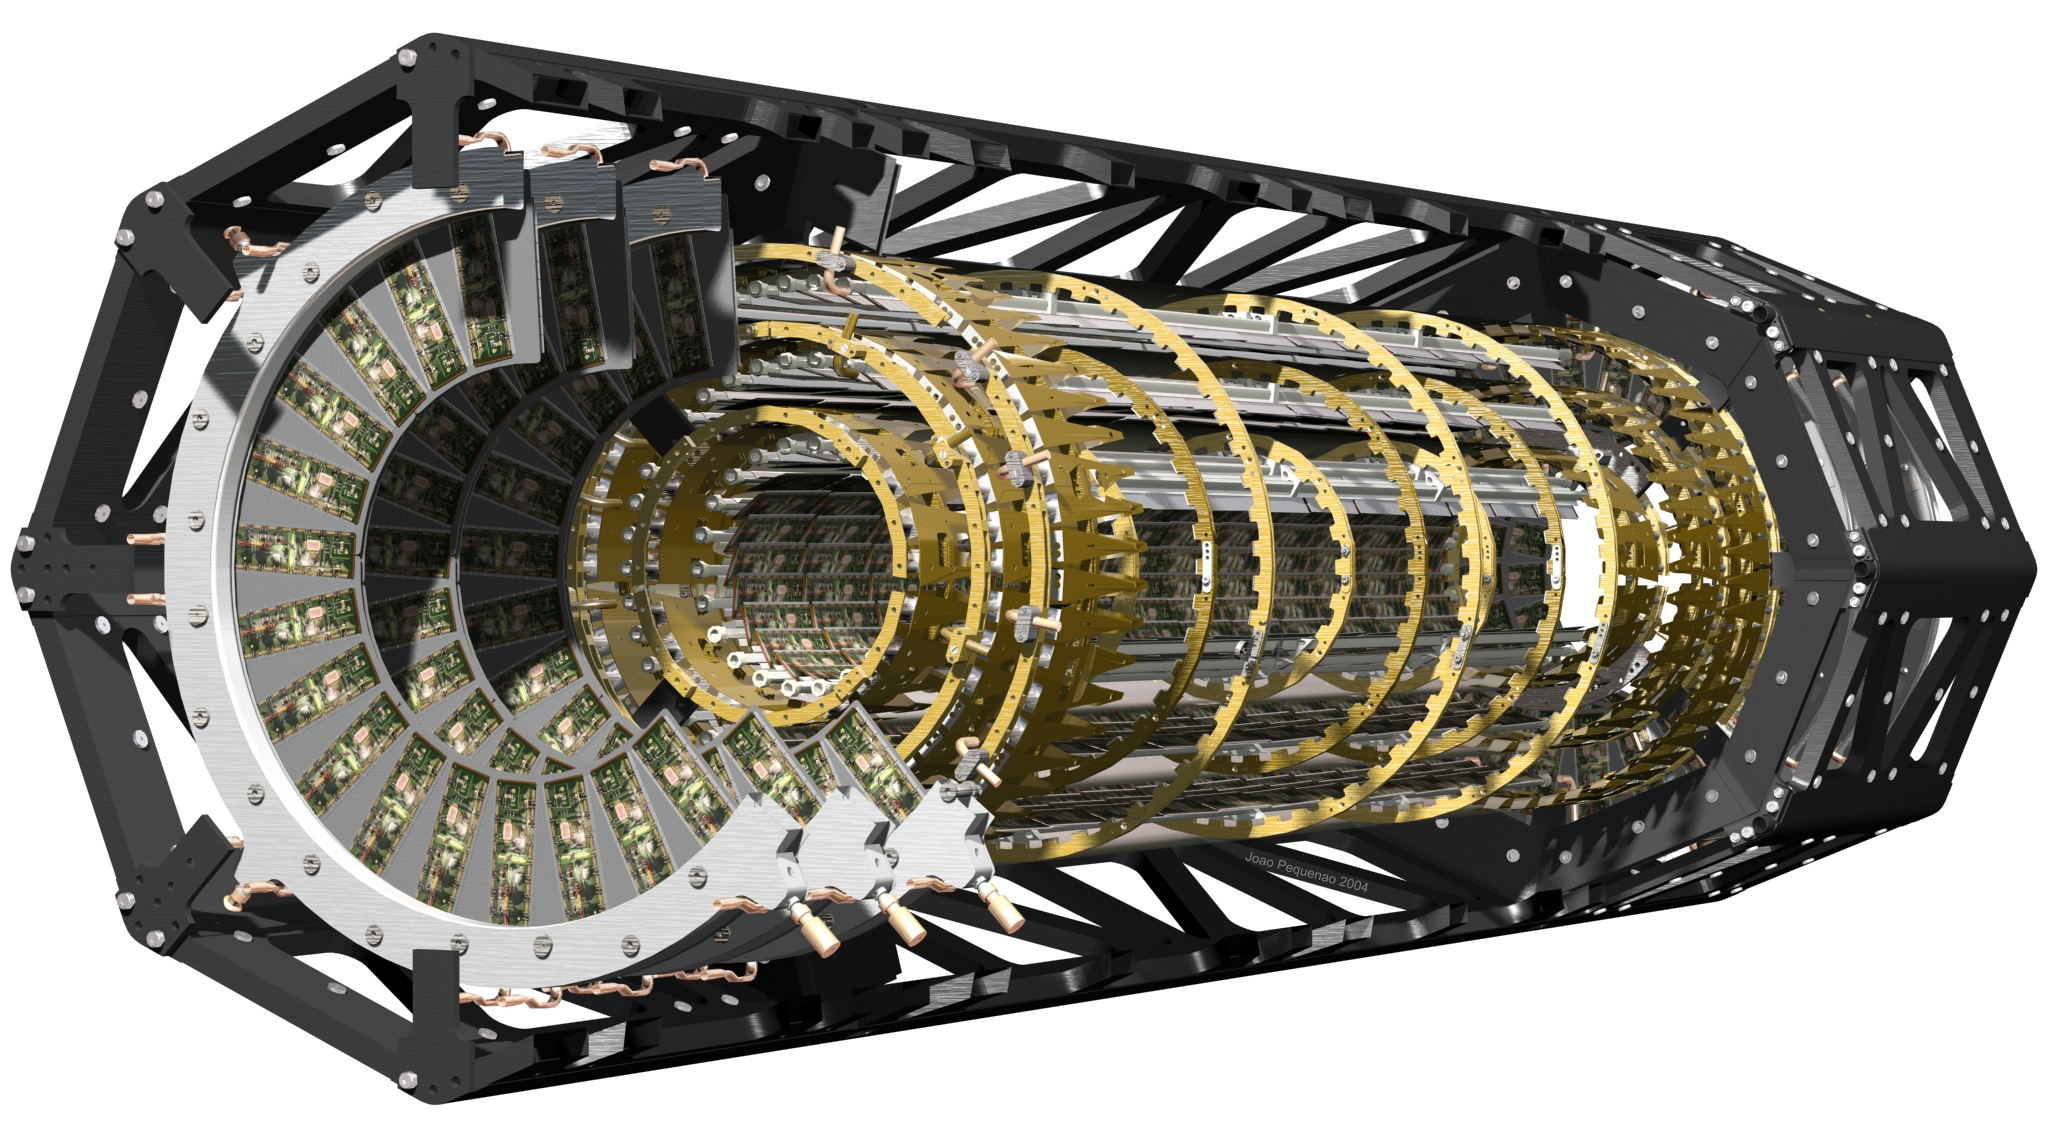
\includegraphics[width=0.65\textwidth]{Images/atlas/Pixel.jpg}}
\subfloat[\label{fig:pixel_module}]{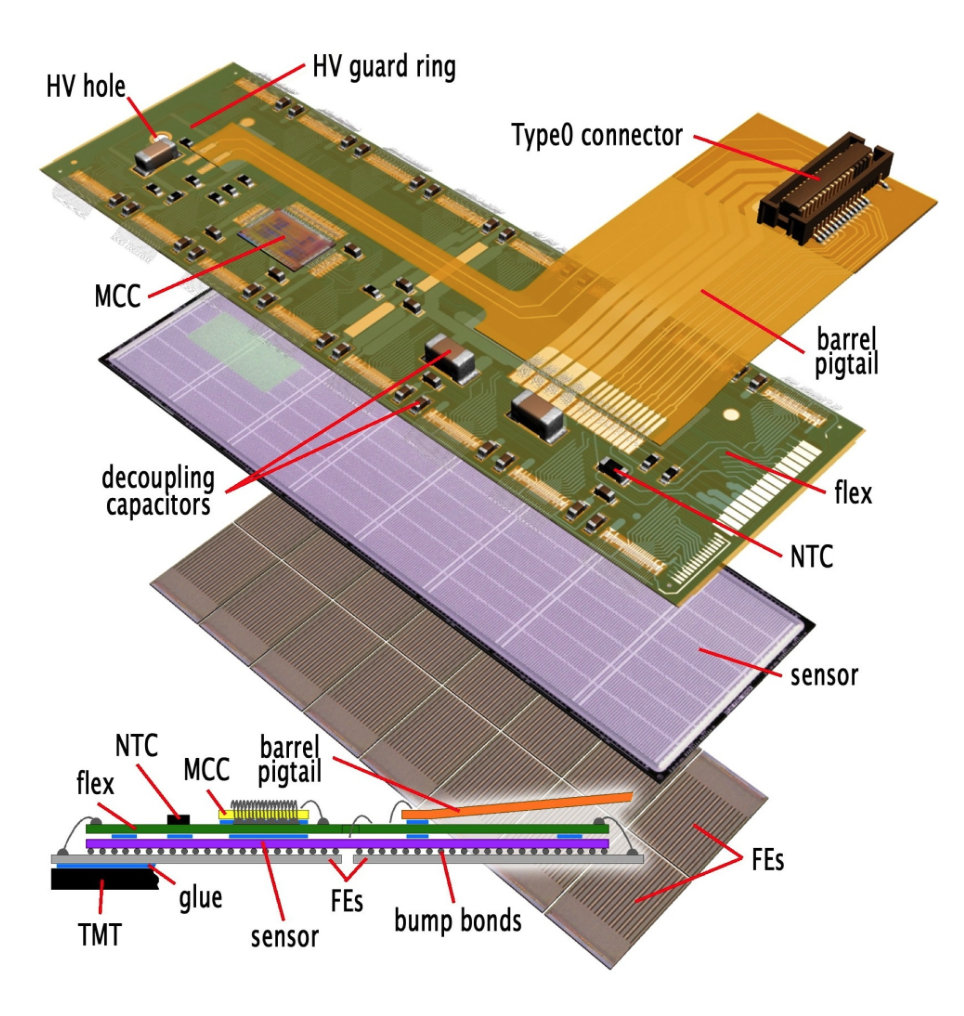
\includegraphics[width=0.35\textwidth]{Images/atlas/pixel_module.png}}
\caption{\subref{fig:atlas_pixel} Engineering drawing of the Pixel Detector. \subref{fig:pixel_module} Schematic view of the FEI3 pixel module}
\end{figure}
The ATLAS Pixel Detector consisted of three barrel layers during \runone, located at 50.5, 88.5 and \SI{122.5}{\milli\meter}, and three disks on either side for the forward direction, at a distance of 495, 580 and \SI{650}{\milli\meter}; a drawing of the layout is shown in Figure~\ref{fig:atlas_pixel}. The Pixel Detector has a full coverage for the $\phi$ angle and up to $\pm$2.5$\eta$ in pseudo-rapidity with  respect to the interaction point.
The three layers are equipped with 1744 identical sensor-chip-hybrid modules, mounted on carbon support structure (staves). This structure guarantees good mechanical and positional stability of the modules during operation while the amount of material has to be kept to a minimum. At the same time it has to provide cooling to remove the heat load of typically \SI{4}{\watt} from the modules and maintain the sensors at a low temperature to keep the radiation damage low. The cooling is provided by a evaporative fluorocarbon system\cite{pixel_cooling}. The total material budget of the entire barrel is approximately 10.7\percent X$_0$ for particle crossing the detector at $\eta = 0$.
A pixel module (Figure~\ref{fig:pixel_module}) consists of a single silicon sensor, with an area of approximately $2\times6$\SI{}{\centi\meter^2} and a thickness of \SI{250}{\micro\meter}. To provide a high space-point resolution of  \SI{\sim12}{\micro\meter} in the $R\phi$ plane and \SI{\sim115}{\micro\meter} along the beam pipe direction, each sensor is subdivided in a pixel matrix. The pixel matrix presents two categories of pixels, the standard one which is \SI{50}{\micro\meter} long in the $R\phi$ direction \SI{400}{\micro\meter} in the z one, and long one which has the same length in $R\phi$ but is \SI{600}{\micro\meter} in the z direction. For each sensors there are 41984 standard pixels and 5248 long ones. The long pixels are located ad the edge of the module to cover the gaps between adjacent front-ends.\\
Each sensor is individually connected to 16 front-end chips (FE-I3)\cite{ale_vertex_3}) using bump-bondings for each pixel. The front-end provides pulse height measurements by means of the Time over Threshold (\tot) with zero suppression on chip. These front-end chips are connected via wire-bonds to a kapton-flex hybrid glued onto the back-side of the sensor. A module-control chip is mounted on top of the flex-hybrid and combines the individual events from the front-end chips and distributes trigger and command signal. The module-control chip is responsible of the communication with the off-detector electronics via optical link. In order to keep the material budget low, both the front-end and the module control-chip are thinned to below \SI{200}{\micro\meter}.

\subsection{Refurbishment and consolidation of the Pixel Detector}
\begin{figure}
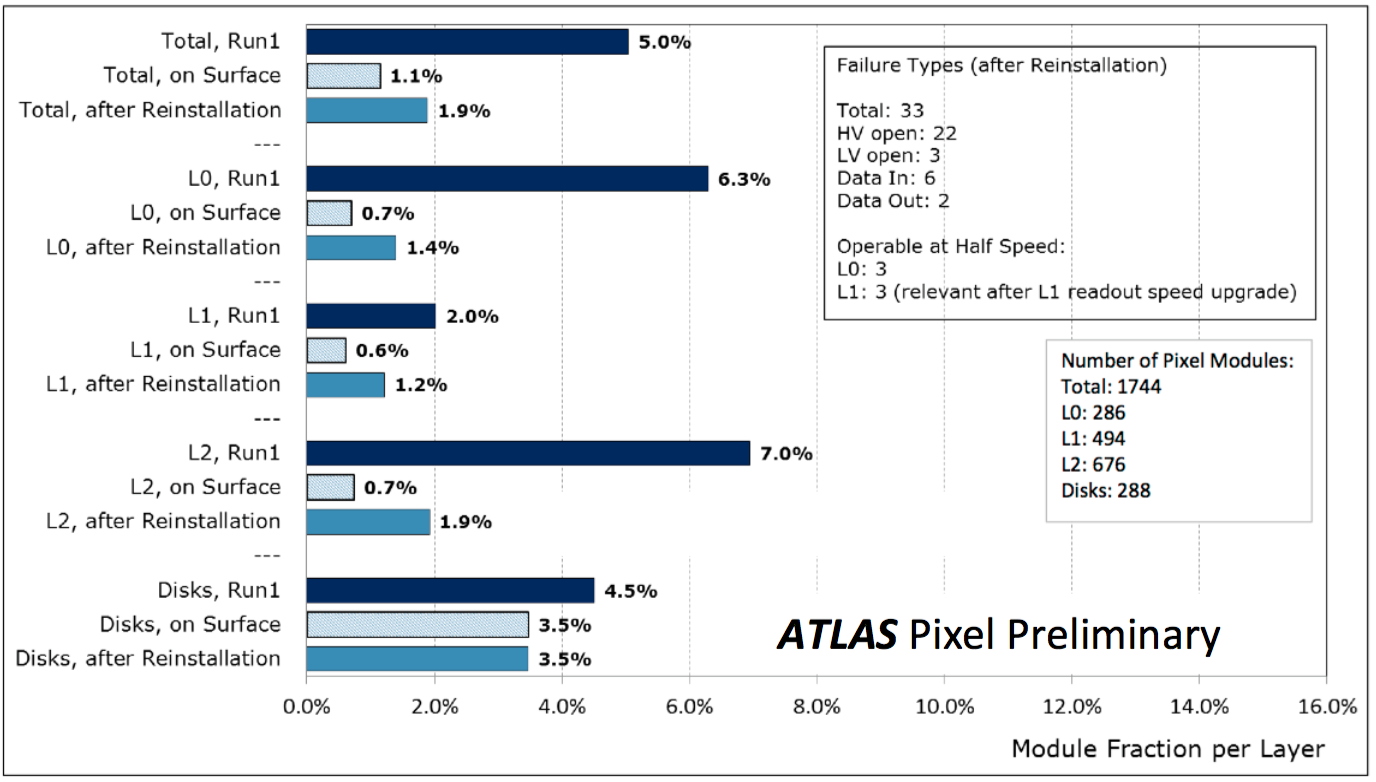
\includegraphics[width=0.8\textwidth]{Images/atlas/pixel_nsqp_performance.png}
\label{fig:nsqp}
\caption{Operational status of pixel module at the end of \runone and after the intervention before the start of \runtwo}
\end{figure}
During the \runone some of the lasers in the off-detector system of the Pixel Detector started to fail, it was then decide to replace the service quarter panel. The same type of laser were also present in the on-detector system (Optoboards) and they cannot be access without removing the Pixel Detector from ATLAS. It was then decided to build new service quarter panels (nSQP) locating the Optoboards into accessible area. The readout speed of the second layer was upgraded to 160Mbit/s, as for the innermost layer.\\
At the end of \runone 95\percent of the pixel module was correctly operating. An investigation was performed for the modules which were failing in the operation, and whereas it was possible, faulty modules were fixed. In May 2014 the Pixel detector has been re-inserted in the ATLAS volume, all the services were connected and after having retested the detector 98\percent of the module was proved to be fully functional. Figure~\ref{nsqp} shows the details about the module recovery.

\subsection{Motivation for the ATLAS IBL detector}
The first long shutdown of the LHC was the opportunity for the ATLAS collaboration to improve the ATLAS Inner Detector performance with the addition of a fourth innermost layer of silicon pixel detectors, the Insertable B-layer (IBL).\\
The ATLAS Pixel Detector will be operational until the third long-shutdown of the LHC machine, foreseen at the end of the year 2023. In this long period some module are expected to fail, without the opportunity of perform any intervention or substitution of those.\\
In particular a loss of data in the Pixel B-layer would seriously deteriorate the impact parameter resolution, directly affecting the b-tagging capabilities. The addition of a fourth layer, close to the beam-pipe, ensures that b-tagging capabilities will not deteriorate in time and it improves b-tagging performance being located closer to the interaction point with respect to the Pixel B-layer as it will be shown in the next sections.\\
During the \runtwo phase collisions happen each \SI{25}{\nano\second}, instead of the \SI{50}{\nano\second} interval used during \runone, the peak luminosity in \runtwo was increased with respect to the one faced in \runone. These upgrade led to the increase of the pile-up. The higher pile-up environment requires redundancy in the measurement of tracks in order to control the fake rate arising from random combinations of clusters in events with high pile-up background.\\
Since the existing envelope allowed only \SI{8.5}{\milli\meter} of radial free space, too small for the insertion of a new layer, the existing  beam pipe has also been replaced by a new pipe of a reduced diameter allowing the insertion of an additional layer. The new Be beam pipe allows the reduction of material budget close to the interaction point. This beam-pipe will be used as well for the HL-LHC upgrade unless and even smaller beam pipe will become possible then.

%\subsection{Expected performance}
%The ATLAS inner detector provides charged particle tracking with high efficiency in the range $|\eta|~$\textless~2.5 and over the full azimuthal range. 
%Given its radial proximity to the collision region, the existing B-layer provides crucial tracking information: the identification of charged tracks and the reconstruction of multiple collision vertices; subsequent precision   measurements of the reconstruction position, resolution, efficiency and track association for both primary and secondary vertices, and measurements of the b-tagging efficiency as a function of light quark jet rejection. In particular, any inefficiency of the B-Layer results in a severe degradation of the ATLAS physics performance. 
%The addition of the IBL will help to preserve the tracking performance and robustness at high luminosity when the B-layer starts to deteriorate from radiation damage, high pile-up occupancy, or the irreparable failure of individual FE-I4 chips or full modules. In addition, given the reduced radial distance to the interaction point and the smaller longitudinal pixel size, the IBL significantly improves the measurement of track transverse ($d_0$) and longitudinal ($z_0 \times$sin$\theta$) impact  parameter resolution.
The improvement of the Pixel Detector performance with the addition of the IBL was carefully evaluated with studies on tracking an b-tagging. Expected performances in tracking and b-tagging are presented in the following two sections.

\subsubsection{Track reconstruction performance}
The impact parameter performance have been evaluated by parametrizing the observed \pt dependence by the $A+\frac{B}{p_T }$ model, for which the A term describes the intrinsic resolution of the detector visible at high \pt , while the B term describes the effect of multiple scattering in the detector material dominant at low \pt.
The IBL improves A by a factor of 1.2 in $d_0$ and a factor of 1.7 in $z_0 \times$sin$\theta$, driven by the change in the $z$ pitch between IBL and current Pixel detectors. The multiple scattering term B improvs by a factor of 1.8 in $d_0$ and as well a factor of 1.8 in $z_0 \times$sin$\theta$. As a consequence of the improved resolution of the impact parameters, the IBL improves the primary vertex resolution and reconstruction, secondary vertex finding, $b$-tagging performance, hence extending the reach of the physics analysis. To assess the direct contribution of IBL, selected Monte Carlo samples have been generated to compare the performance of the track detector at the end of Run~1 with that at the start of Run~2, using the same boundary conditions (e.g. disabled pixel modules, pile-up and collision energy).
Figure~\ref{fig:runtwoDegradation} shows how the IBL will compensate for the expected B-Layer degradation with radiation and occupancy at the end of Run~2.

%\begin{figure}
%	\centering
%
\includegraphics[width=\textwidth]{Images/IBL_paper/chapter05_Staves/PlaceHolder.jpg}
%  \caption{Fakes runone vs runtwo.}
%  \label{fig:runonevsruntwo}	
%\end{figure}

\begin{figure}
\centering
\vspace{-4cm}
 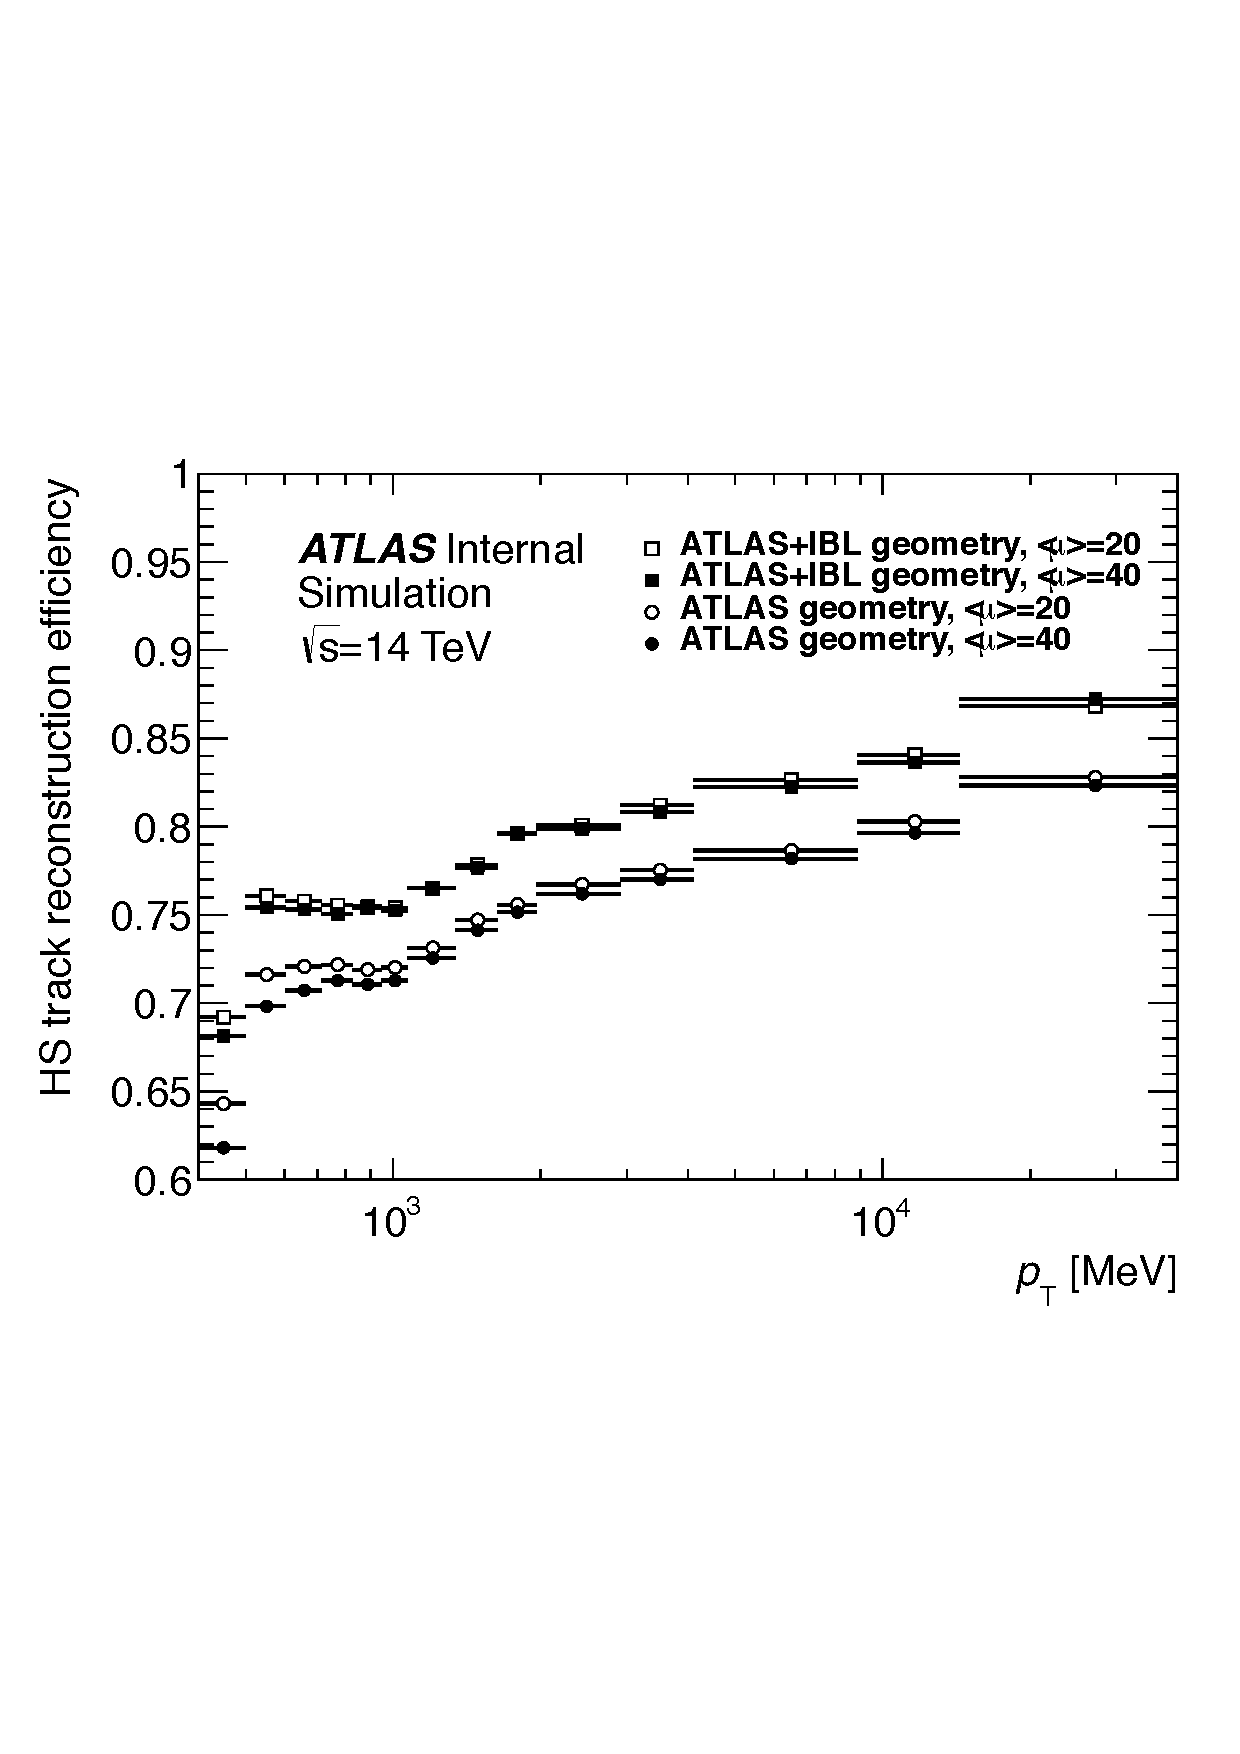
\includegraphics[width=0.7\textwidth]{Images/IBL_paper/chapter02_Physics/TrackingEff.pdf}
\vspace{-4cm}
\caption{runtwo  degradation performances.}
\label{fig:runtwoDegradation}

\end{figure}

\subsubsection{$b$-tagging performance}
\label{sec:btagperformance}

Thanks to the significantly improved impact parameter resolution, the IBL has a major impact on the $b$-tagging performance. In this section a comparison is presented between the $b$-tagging performance expected after the addition of IBL and what was achieved at the end of \runone.
The performance was evaluated with the use of the updated digitization model and reconstruction algorithms, which were both improved for the \runtwo.
The latter include a refined neural network clustering algorithm~\cite{Aad:2014yva}, a new tracking setup which improves the treatment of shared clusters in the core of a dense jet environment~\cite{ATL-PHYS-PUB-2015-006} and a new $b$-tagging algorithm.
%This super-seeds the results presented in the IBL TDR~\cite{Capeans:1291633}, with the use of a more realistic simulation of the inner tracking detector based on the final IBL geometry, an updated digitization model and significantly improved reconstruction algorithms. The latter include a refined neural network clustering algorithm~\cite{Aad:2014yva}, a new tracking setup which improves the treatment of shared clusters in the core of a dense jet environment~\cite{ATL-PHYS-PUB-2015-006} and a new $b$-tagging algorithm, which will be briefly described in the following.

All results presented here are based on fully simulated top pair production events. The average level of pile-up in this study is $\approx 20$, reflecting the \runone luminosity profile. The dependence on pile-up is studied separately. Jets are reconstructed with the AntiKt algorithm~\cite{AntiKt} with radius R~$=0.4$. The $b$-tagging algorithms used in the ATLAS experiment rely on a combination of three basic algorithms:
\begin{itemize}
\item{Impact parameter based}
\item{Inclusive secondary vertex reconstruction}
\item{Decay chain multi-vertex reconstruction}
\end{itemize}
The impact parameter based algorithm relies on the impact parameter significance and lifetime sign of the single tracks matched to the jet, which are then combined in a single likelihood discriminator. The secondary vertex based algorithm exploits explicitly the presence of a secondary vertex within the jet and of its properties, including mass, energy fraction and charged decay multiplicity. Finally, the multi-vertex fitting algorithm tries to reconstruct the PV~$\to b$-$\to c$-hadron decay chain expected in most of the $b$-jets, exploiting its topology and properties. A detailed description of the basic algorithms can be found in Chapter 7.% For the impact parameter based algorithm the categorization of tracks has been significantly refined with respect to the version used in \runone.

\begin{figure}
\centering
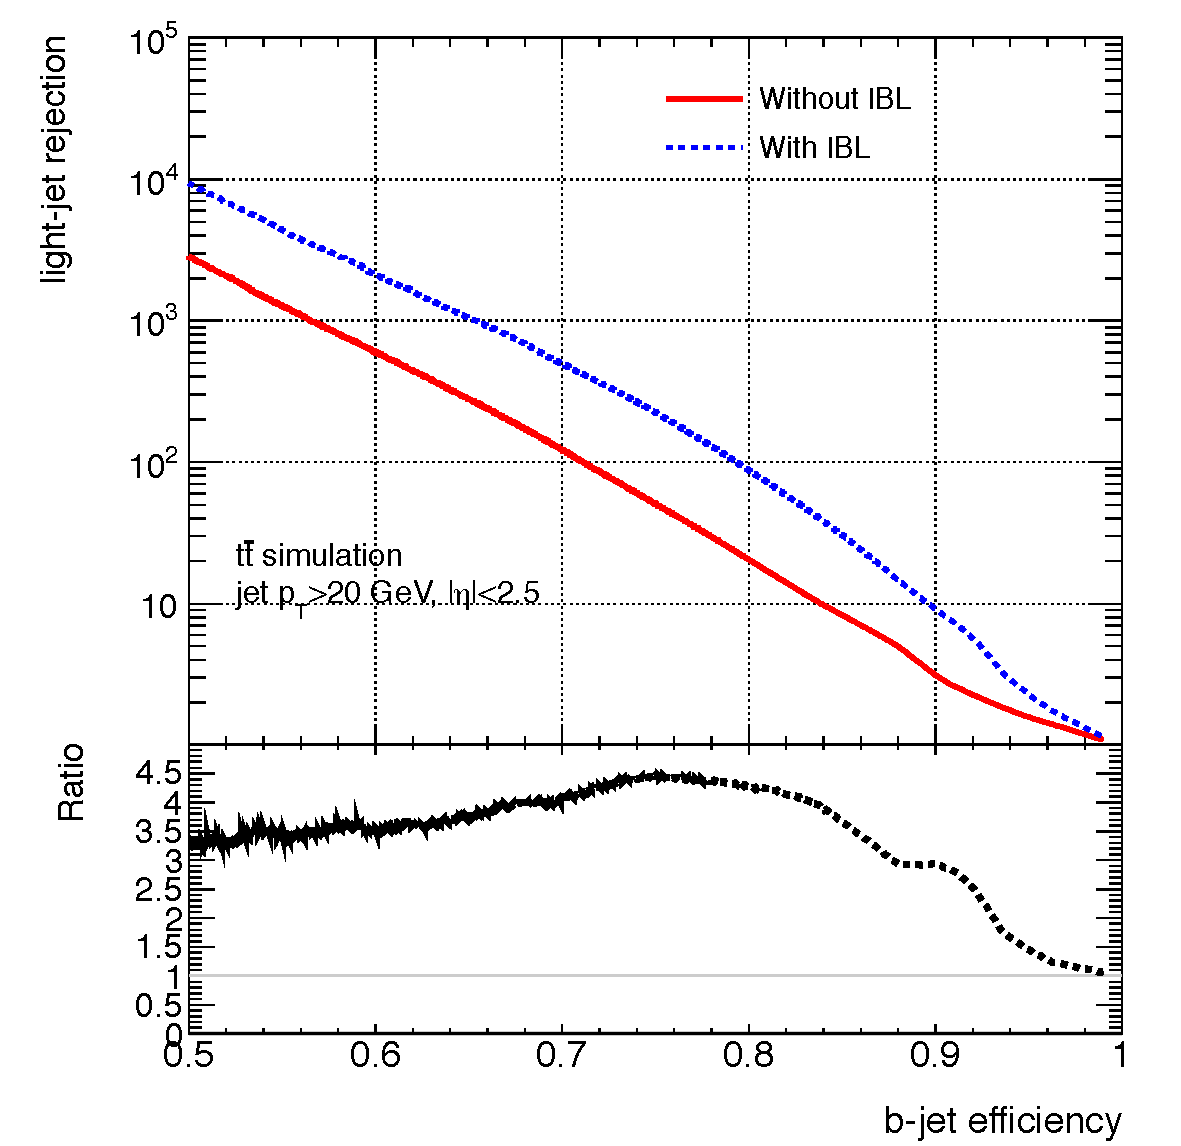
\includegraphics[width=0.45\textwidth]{Images/IBL_paper/chapter02_Physics/btagging/bVSlight__MV2c20.pdf}
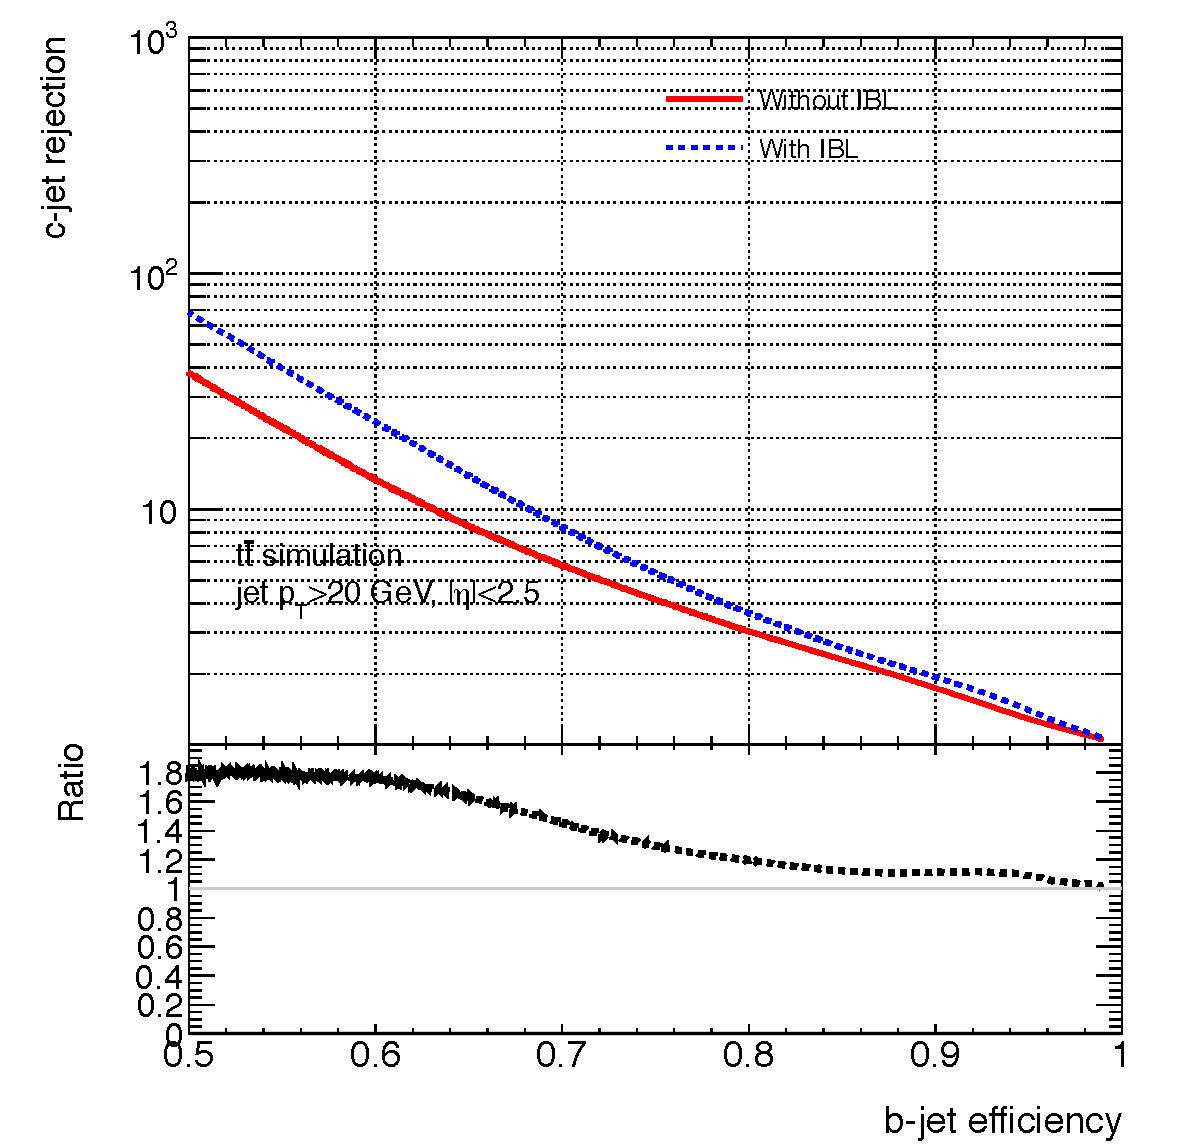
\includegraphics[width=0.45\textwidth]{Images/IBL_paper/chapter02_Physics/btagging/bVSc__MV2c20.pdf}
\caption{\label{fig:btagging_inclusiveROCcurve} Performance of the $b$-tagging algorithm MV2c20 expressed in terms of light (on the left) or $c$-jet (on the right) rejection as a function of $b$-tagging efficiency, obtained by scanning the BDT discriminant. The algorithm is applied to jets from top pair events. The performance of the \runone and \runtwo detector layouts are compared, where the latter includes IBL. The rejection is defined as $R=1/\epsilon$, with $\epsilon$ being the tagging efficiency.}
\end{figure}

The input variables obtained from the three basic algorithms are then combined making use of a boosted decision tree algorithm to discriminate $b$-jets from either light ($u$,$d$,$s$-quark or gluon jets) or $c$-jets. Results in this sections are presented for the MV2c20 algorithm, for which the training is performed on a set of at least 5 million top pair events, using the $b$-jets as signal and a mixture of 80\% light-jets and 20\% $c$-jets as background. In order to perform a fair comparison, the algorithms have been re-trained separately for the ATLAS \runone geometry, without IBL, and the ATLAS \runtwo geometry, which includes the IBL.

The inclusive $b$-tagging performance on top pair events, after a very basic jet selection ($p_{T}>20$~GeV and $|\eta|$<2.5\%), is shown in Figure~\ref{fig:btagging_inclusiveROCcurve}. The additional of IBL improves the $b$-tagging performance in terms of light-jet rejection between a factor of 3 or 4 for $b$-jet tagging efficiencies up to 85\%.  The improvement in $c$-jet rejection is smaller and ranges approximately from 80\% to 20\% for $b$-jet tagging efficiencies from 50 to 75\%. Physics analyses will most often profit from the improved performance by re-tuning their $b$-tagging requirements in such a way to keep the background rejection the same but have an increased signal efficiency: this is shown in Table~\ref{tab:btagging_fixedRejection}. As an example, adding the IBL allows to keep the light-jet rejection rate at 100 while improving the $b$-jet tagging efficiency from 72\% to 79\%, with a relative improvement of 10\% on the $b$-tagging efficiency for each tagged jet in the event.

\begin{table}
\begin{center}
\begin{tabular}{lccc}
\hline
Light-jet rejection                                     & $b$-jet efficiency w/o IBL & $b$-jet efficiency with IBL \\ \hline
1000                                                            & 57\%     & 65\% \\
100                                                            & 71\%     & 79\% \\
10                                                            & 84\%     & 90\% \\ \hline
\hline
Constant $c$-jet rejection                                     & $b$-jet efficiency w/o IBL & $b$-jet efficiency with IBL \\ \hline
20                                                            & 56\%     & 62\% \\ 
10                                                            & 63\%     & 68\% \\ 
5                                                              & 72\%     & 76\% \\ \hline
\end{tabular}
\caption{\label{tab:btagging_fixedRejection} $B$-jet tagging performance expressed in terms of $b$-jet efficiency for a fixed light- or $c$-jet rejection, comparing the \runone and \runtwo detector layouts, where the latter includes IBL, and as derived from jets from top pair production, which pass the $p_{T}>20$~GeV and $|\eta|<2.5$ selection requirements.}
\end{center}
\end{table}

The $b$-tagging performance depends strongly on jet transverse momentum ($p_{T}$),
%and pseudo-rapidity ($\eta$), 
following the variation in underlying impact parameter resolution and tracking efficiency. The dependence of the performance on jet $p_{T}$ is shown in Figure~\ref{fig:btagging_vsPT}.
%, while the dependence on $\eta$ is shown in Figure~\ref{fig:btagging_vsETA}. 
The largest improvements are seen at low $p_{T}$, where the closeness of the IBL to the interaction region allows to reduce significantly the impact of multiple scattering. As an example, the improvement in light-jet rejection ranges from a factor of 3-4 up to $p_{T}=100$~GeV, a factor of 2 at $p_{T}=150$~GeV, leveling to only a very slight  improvement for jet $p_{T}$ above 250 GeV. At very high jet $p_{T}$ the tracking efficiency and resolutions are limited by shared clusters from collimated tracks produced in the core of high $p_{T}$ jets, a problem which becomes more severe with the insertion of IBL, which moves the radial distance of the closest pixel layer to the interaction region from $\approx 5$ to $\approx 3.3$~cm. The optimization of the tracking and pixel clustering algorithms to deal with such an environment~\cite{Aad:2014yva,ATL-PHYS-PUB-2015-006} has allowed to counteract such degradation effectively and keep the performance of the new \runtwo geometry at least at the same level of \runone even for very high $p_{T}$ jets. 

%{\bf Need to understand first bin in $p_{T}$ (especially for c-jets !!) and the last bins in $\eta$.}

\begin{figure}
\centering
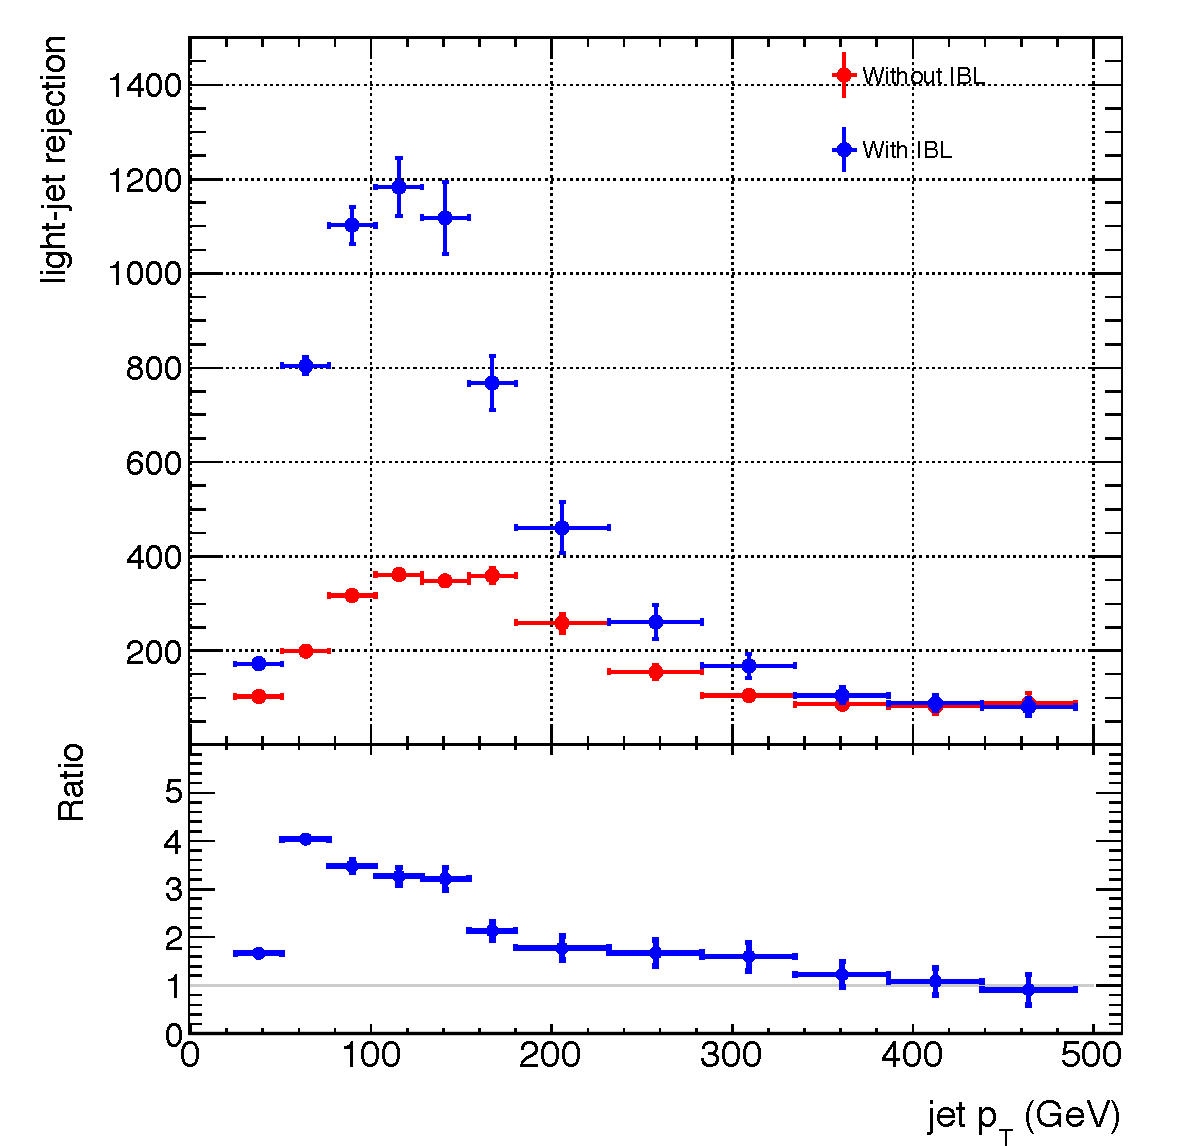
\includegraphics[width=0.45\textwidth]{Images/IBL_paper/chapter02_Physics/btagging/jet_pt_MV2c20__l_flat}
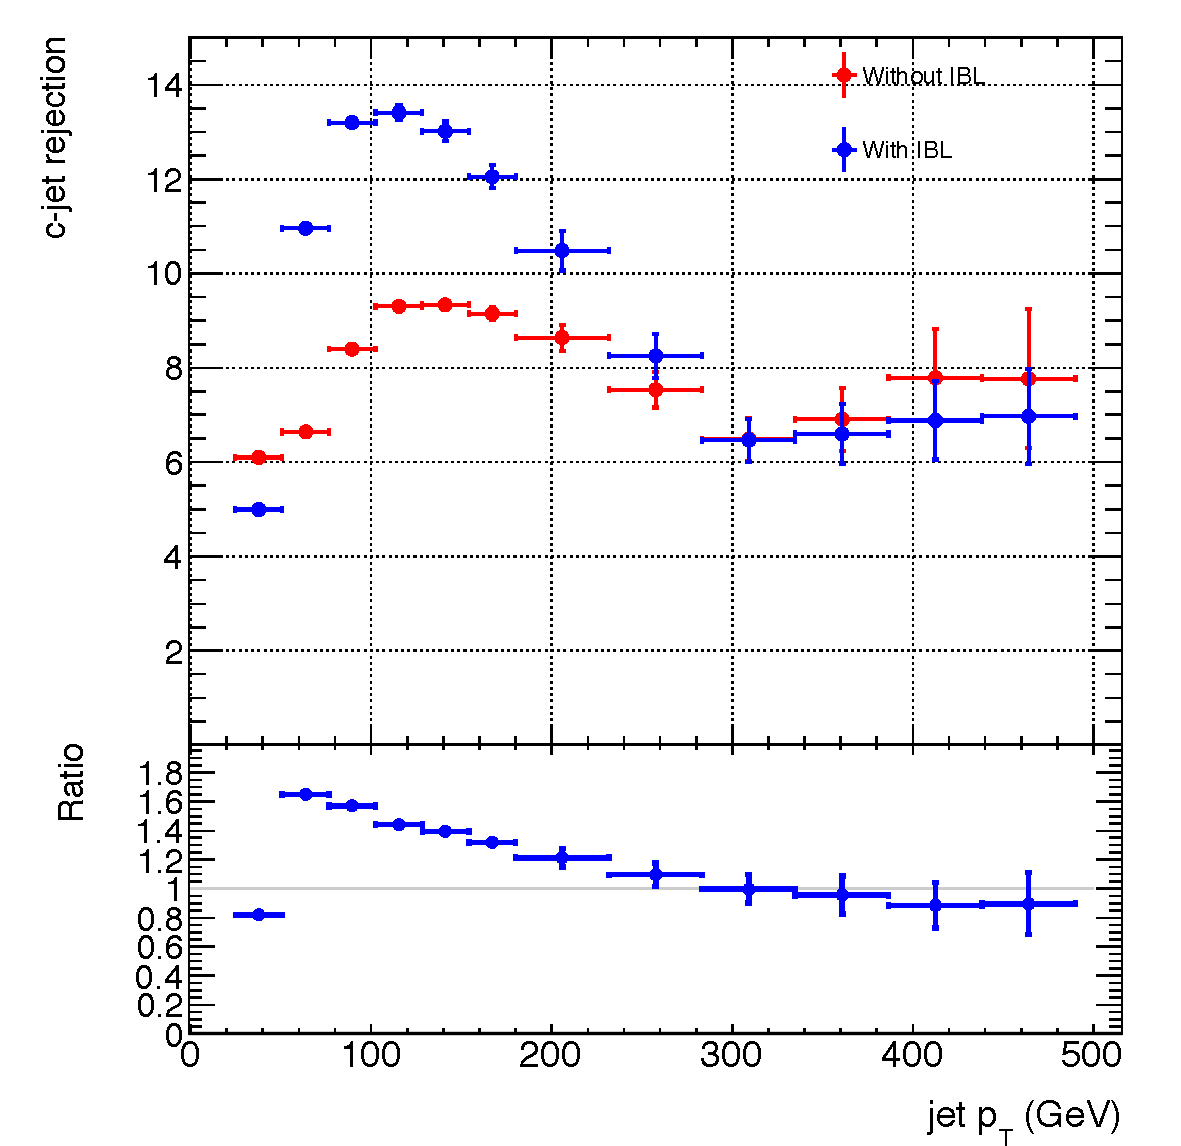
\includegraphics[width=0.45\textwidth]{Images/IBL_paper/chapter02_Physics/btagging/jet_pt_MV2c20__c_flat}
\caption{\label{fig:btagging_vsPT} Performance of the $b$-tagging algorithm MV2c20 expressed in terms of light (on the left) or $c$-jet (on the right) rejection as a function of jet transverse momentum ($p_{T}$), while keeping the $b$-tagging efficiency fixed at 70\% in each $p_{T}$ bin. The performance of the \runone and \runtwo detector layouts are compared, where the latter includes IBL. The rejection is defined as $R=1/\epsilon$, with $\epsilon$ being the tagging efficiency.}
\end{figure}

%\begin{figure}[htb!]
%\centering
%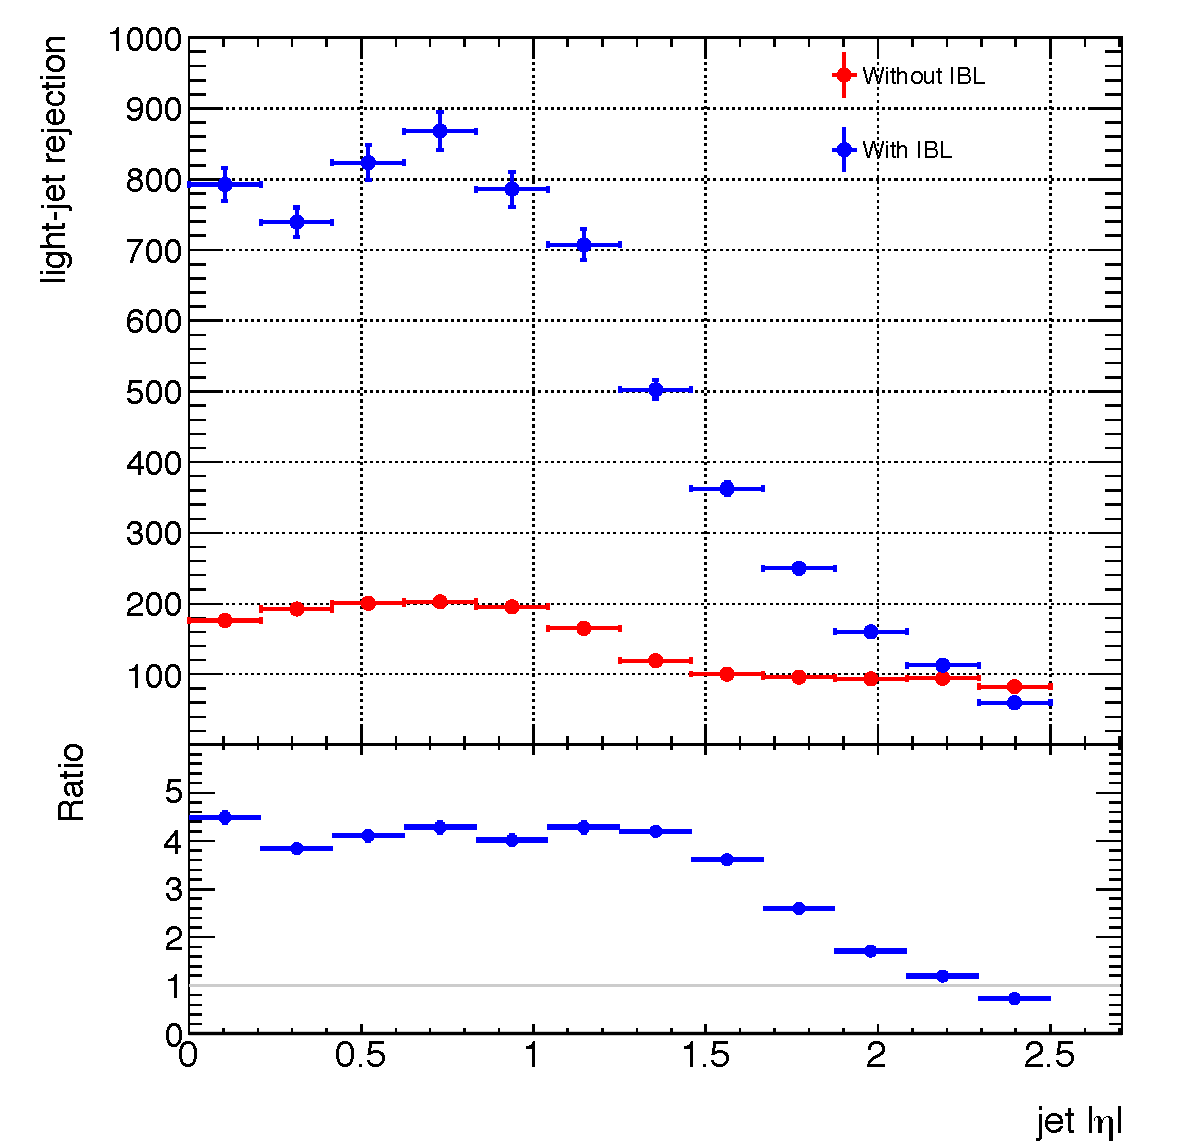
\includegraphics[width=0.45\textwidth]{Images/IBL_paper/jet_eta_MV2c20__l_flat}
%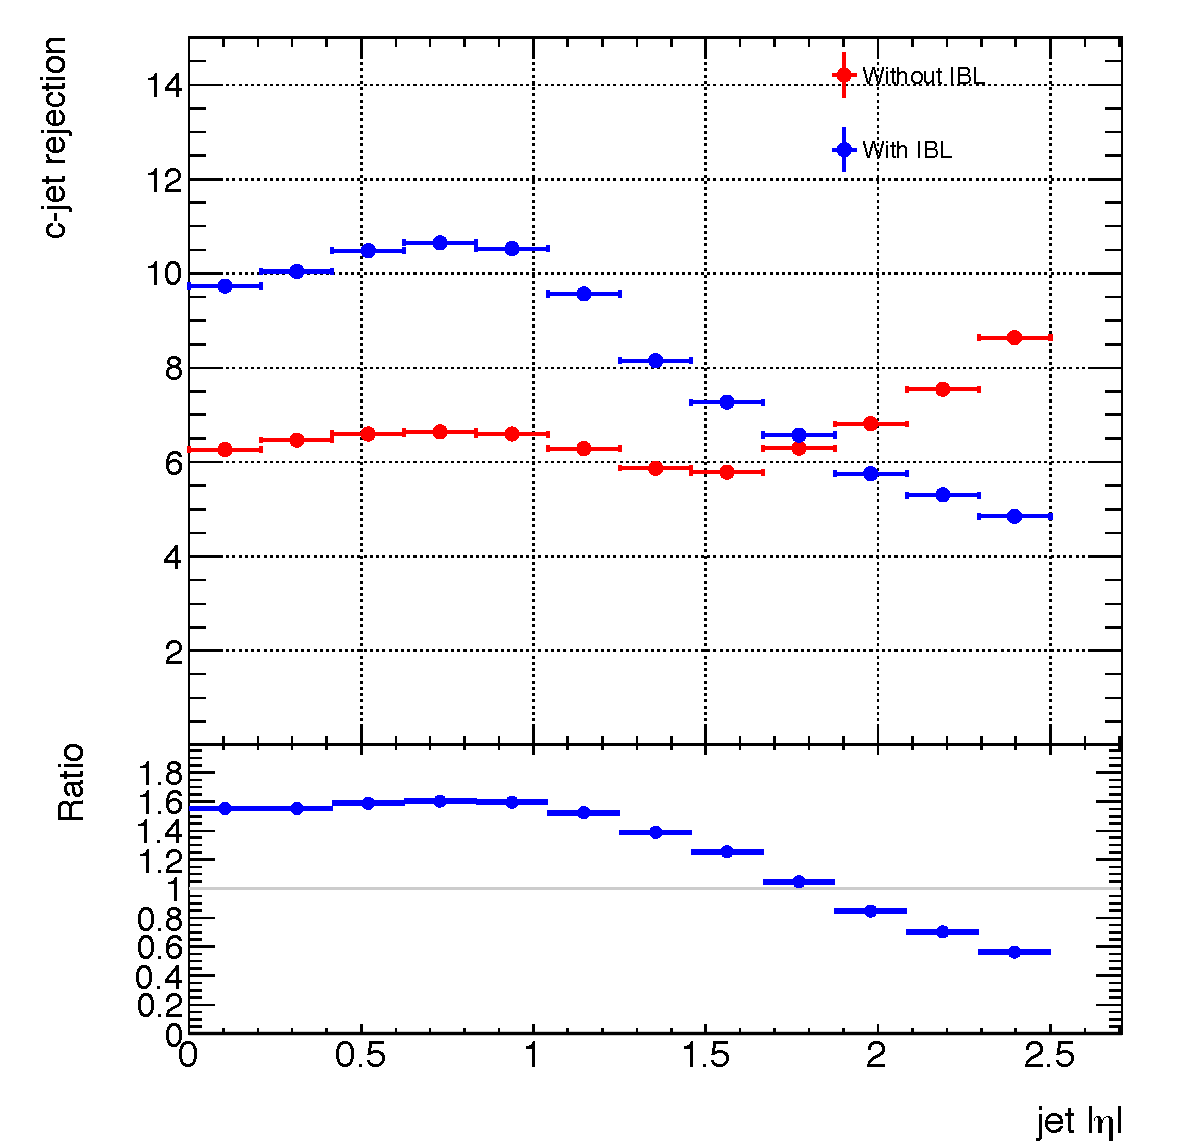
\includegraphics[width=0.45\textwidth]{Images/IBL_paper/jet_eta_MV2c20__c_flat}
%\caption{\label{fig:btagging_vsETA} Performance of the $b$-tagging algorithm MV2c20 expressed in terms of light (on the left) or $c$-jet (on the right) rejection as a function of jet pseudo-rapidity ($\eta$), while keeping the $b$-tagging efficiency fixed at 70\% in each $\eta$ bin. The performance of the \runone and \runtwo detector layouts are compared, where the latter includes IBL. The rejection is defined as $R=1/\epsilon$, with $\epsilon$ being the tagging efficiency.}
%\end{figure}

The dependence on the average level of pile-up $\mu$ is presented in Figure~\ref{fig:btagging_vsMU}. While the overall performance is much improved with the addition of IBL, the dependence on pile-up in terms of relative degradation versus $\mu$ is almost unchanged, except in the case of the $c$-jet rejection, where a more severe degradation is seen with the IBL inserted. This study is performed on top pair events, where the distinction of the primary vertex from pile-up vertices is not a major concern.

\begin{figure}
\centering
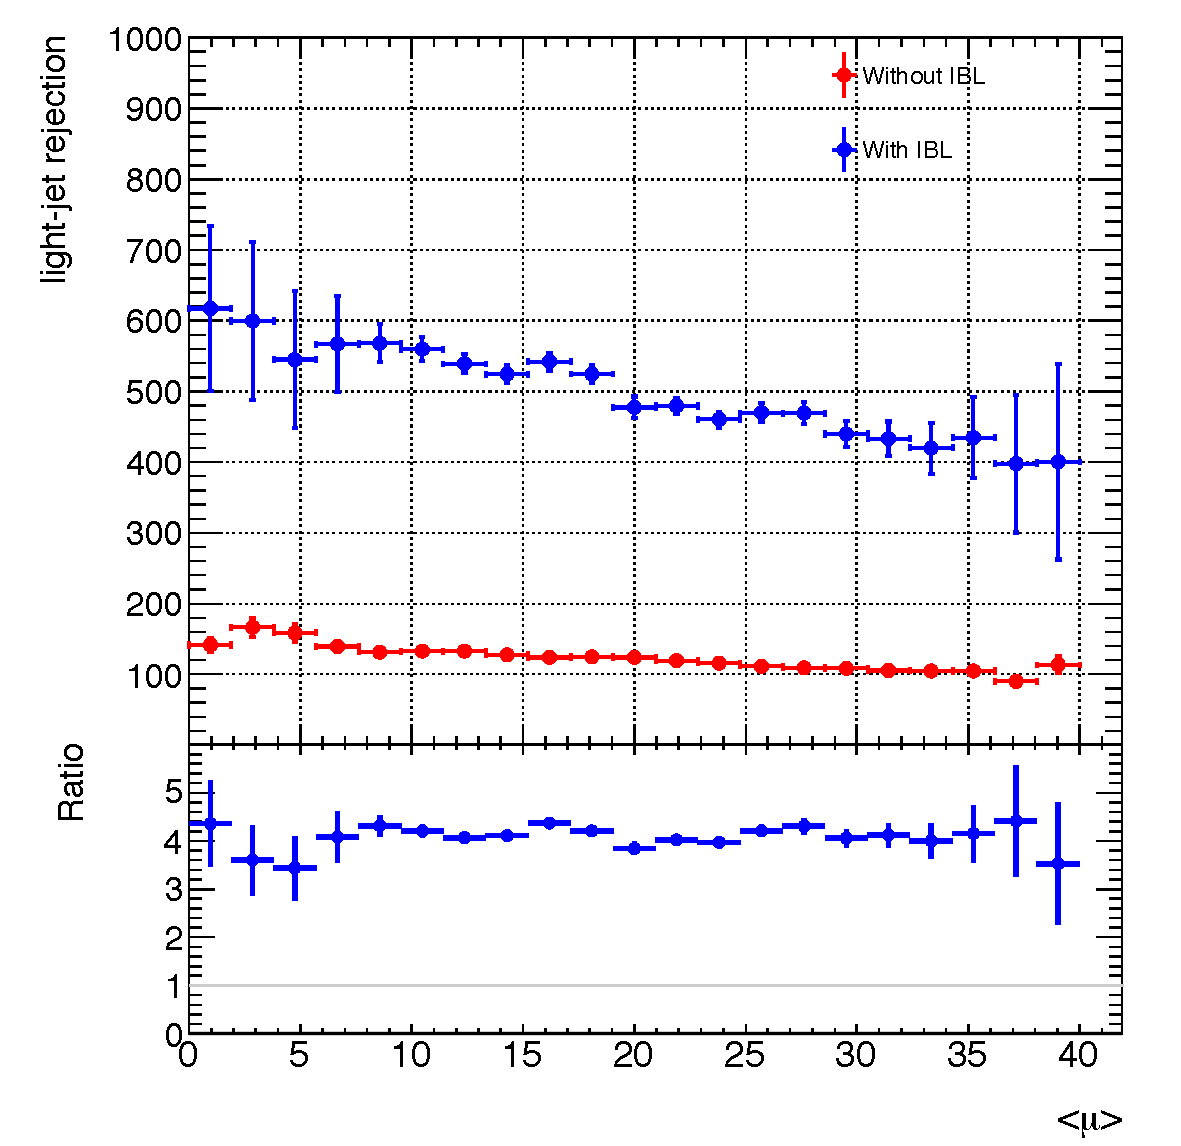
\includegraphics[width=0.45\textwidth]{Images/IBL_paper/chapter02_Physics/btagging/avgmu_MV2c20__l_flat}
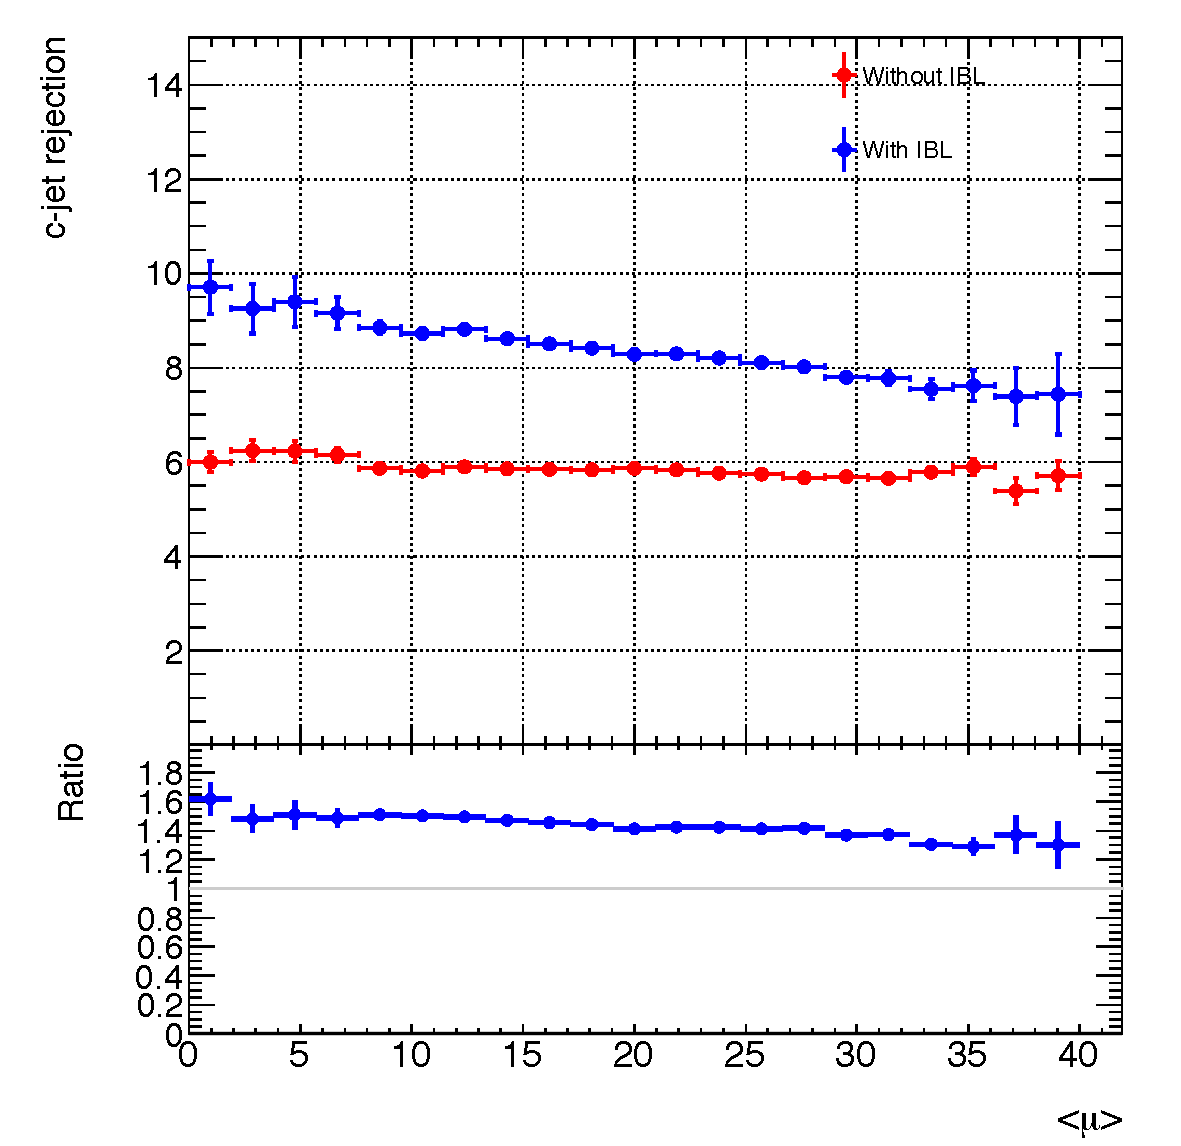
\includegraphics[width=0.45\textwidth]{Images/IBL_paper/chapter02_Physics/btagging/avgmu_MV2c20__c_flat}
\caption{\label{fig:btagging_vsMU} Performance of the $b$-tagging algorithm MV2c20 expressed in terms of light (on the left) or $c$-jet (on the right) rejection as a function of the average pile-up level $\mu$, while keeping the $b$-tagging efficiency fixed at 70\% in each $\mu$ bin. The performance of the \runone and \runtwo detector layouts are compared, where the latter includes IBL. The rejection is defined as $R=1/\epsilon$, with $\epsilon$ being the tagging efficiency.}
\end{figure}


%\begin{figure}
%  \begin{center}
%  \includegraphics[width=0.5\textwidth]{2d-cut.pdf}
%  \caption[JetFitterCharm 2-dimensional cut plane]{
%Two-dimensional distribution of the JetFitterCharm anti-$b$ ($\log(P_c/P_b)$) and anti-light ($\log(P_c/P_{\rm light})$) discriminants. The density of red, green, and blue reflect the density of $b$, $c$, and light jets, white areas are a mix of all three \flavours, whereas black areas lack any jets. The `medium' calibrated operating point selects jets above a certain threshold in both anti-$b$ and anti-light discriminants.
%Ridge structures arise from two features of the algorithm which concentrate values in the input space. The first feature is the use of discrete kinematic bin inputs, $\eta^{\rm cat}$ and $\pt^{\rm cat}$. The second is the substitution of default values when the ordinary input values would not be physically meaningful, for example when no secondary vertex is found. The resulting high density structures can be seen in the lower-center and upper-left region of the plot.}
%  \label{fig:2dcut}
%  \end{center}
%\end{figure}




%\begin{figure}
%  \begin{center}
%  \includegraphics[width=0.5\textwidth]{2d-cut.pdf}
%  \caption[JetFitterCharm 2-dimensional cut plane]{
%Two-dimensional distribution of the JetFitterCharm anti-$b$ ($\log(P_c/P_b)$) and anti-light ($\log(P_c/P_{\rm light})$) discriminants. The density of red, green, and blue reflect the density of $b$, $c$, and light jets, white areas are a mix of all three \flavours, whereas black areas lack any jets. The `medium' calibrated operating point selects jets above a certain threshold in both anti-$b$ and anti-light discriminants.
%Ridge structures arise from two features of the algorithm which concentrate values in the input space. The first feature is the use of discrete kinematic bin inputs, $\eta^{\rm cat}$ and $\pt^{\rm cat}$. The second is the substitution of default values when the ordinary input values would not be physically meaningful, for example when no secondary vertex is found. The resulting high density structures can be seen in the lower-center and upper-left region of the plot.}
%  \label{fig:2dcut}
%  \end{center}
%\end{figure}


%\begin{table}
%\begin{center}
%\begin{tabular}{c|c c | c c c }
%%% \multicolumn{6}{c}{$\charm$-tagging} \\ \hline
%Operating Point & $\log (P_\charm / P_\bottom$) & $\log (P_\charm / P_\light$) & $\epsilon_\charm$ & $1/\epsilon_\bottom$ & $1/\epsilon_\light$ \\ \hline
%Loose & $> -0.9$ & -- & 0.95 & 2.5 & 1.0 \\
%Medium & $> -0.9$ & $> 0.95$ & 0.20 & 8.0 & 200 \\
%\end{tabular}
%\caption[\ctagging operating points]{\ctagging operating points. Charm tagging requires two cuts: one to reject \bottom jets, and another to reject light jets. The approximate efficiency for \charm jets along with the rejection for \bottom and \light jets, with $\pt > 20\,\text{GeV}$ and $|\eta| < 2.5$ as estimated on $\ttbar$ events, are also given.}
%%GP Dan, are the efficiencies estimated on ttbar events?
%\label{tab:ops}
%\end{center}
%\end{table}

%GP temporary, just not to have the references on top




%The IBL upgrade was also combined to the replacement of the beam pipe, a l
\subsection{IBL Layout Overview}
% Chapter coordination:

%During the first long shutdown of the LHC machine, a new pixel layer was added between the Pixel B-layer and the beam pipe in the ATLAS detector.
The IBL is located at a nominal distance of \SI{33.5}{\milli\meter} from the beam axis, where this distance refers to the sensors position and it is the closest layer to the interaction point of the ATLAS Detector as shown in  Figure~\ref{fig:NewID}. Given the small sensor distance from the beam axis (compared with \SI{50.5}{\milli\meter} for the Pixel B-Layer), the sensors and front-end electronics must cope with a much higher hit rate and radiation with respect to the other layers.%and maximum radiation doses of respectively  \SI{5e15}{\nq} non ionizing energy loss (NIEL) and  \SI{250}{\mega\radian} total ionizing dose (TID) during \runone operation.
To address these requirements, a new front-end read-out chip has been developed, the FE-I4~\cite{fei4_manual} and two silicon sensor technologies were developed.\\
%The FE-I4 specifications satisfy the requirements of radiation tolerance and read out efficiency at high luminosity. In addition, the FE-I4 chip has a substantially larger active area compared with that of the existing FE-I3\footnote{The FE-I3 is the chip that is used for the other layers of the Pixel Detector} front-end pixel chip and  the pixel size has been reduced to $\SI{250}{} \times \SI{50}{\micro\meter\squared}$. 
\begin{table}
\centering
\begin{tabular}{lc}
\hline \hline
	 & Value\\
\hline
Number of staves & 14 \\
Number of physical modules per stave & 20  (12 Planar, 8 3D)\\
%Number of DCS modules per stave & 16 \\
Number of FEs per stave & 32 \\
Coverage in $\eta$, no vertex spread & $|\eta|\,<\,3.0$ \\
Coverage in $\eta$, 2$\sigma$ (\SI{122}{\milli\meter}) vertex spread & $|\eta|\,<\,2.58$ \\
Active $|z|$ stave length (\SI{}{\milli\meter}) & 330.15 \\
Geometrical acceptance in $z$ min, max (\%) & 97.4, 98.8 \\
Stave tilt in $\phi$ (degree) & 14 \\
Overlap in $\phi$ (degree) & 1.82 \\
Center of the sensor radius (\SI{}{\milli\meter}) & 33.5 \\
Radiation length at $z$ = 0  (\SI{}{\xzero}) & 1.9\\
\hline \hline
\end{tabular}	
\caption{Main layout parameters for the IBL detector. The quoted radiation length is averaged over the stave width and includes the IBL support and positioning tubes.
\label{tab:LayoutTable}}
\end{table}


%The sketch in Figure~\ref{fig:IBLView2} represents the IBL detector and its services. 

\begin{figure}
\begin{center}
 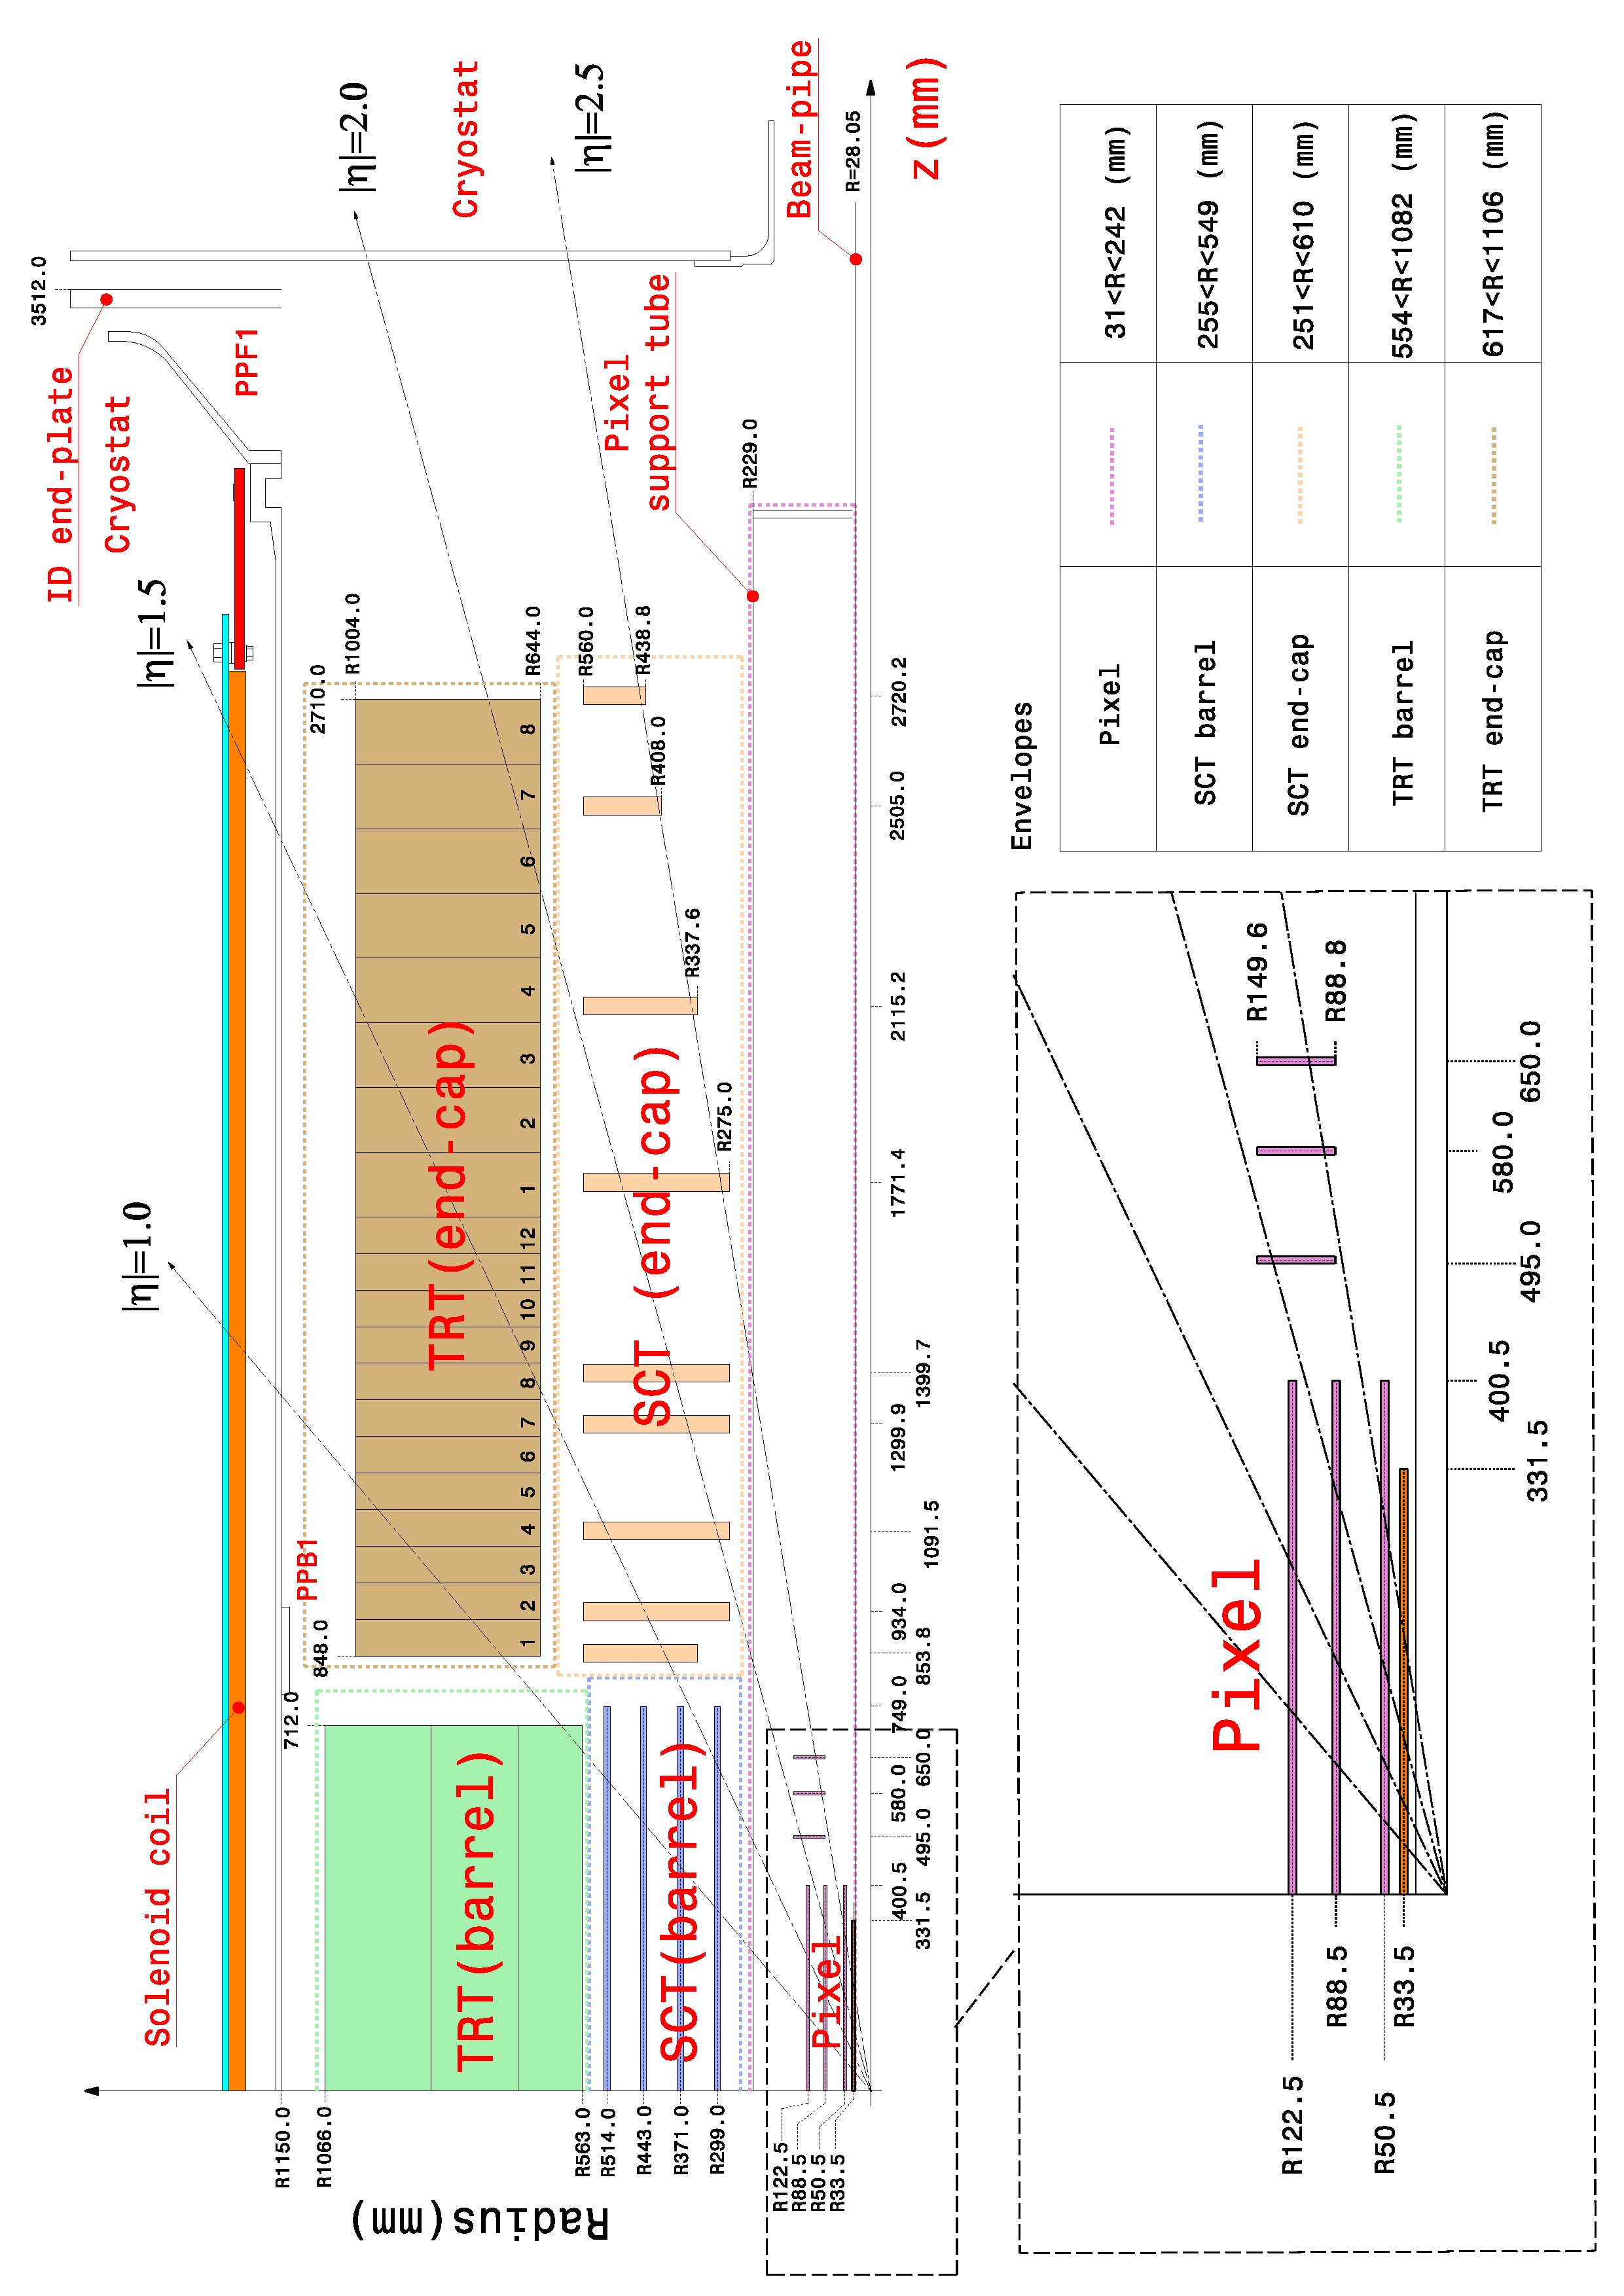
\includegraphics[width=0.61\textwidth, angle = -90 ]{Images/ibl_paper/chapter03_Overview/NewID.pdf}
\caption{The layout of the ATLAS tracking system with the additional layer of IBL. }
\label{fig:NewID}
\end{center}
\end{figure}


%\begin{figure}[!htb]
%\begin{center}
%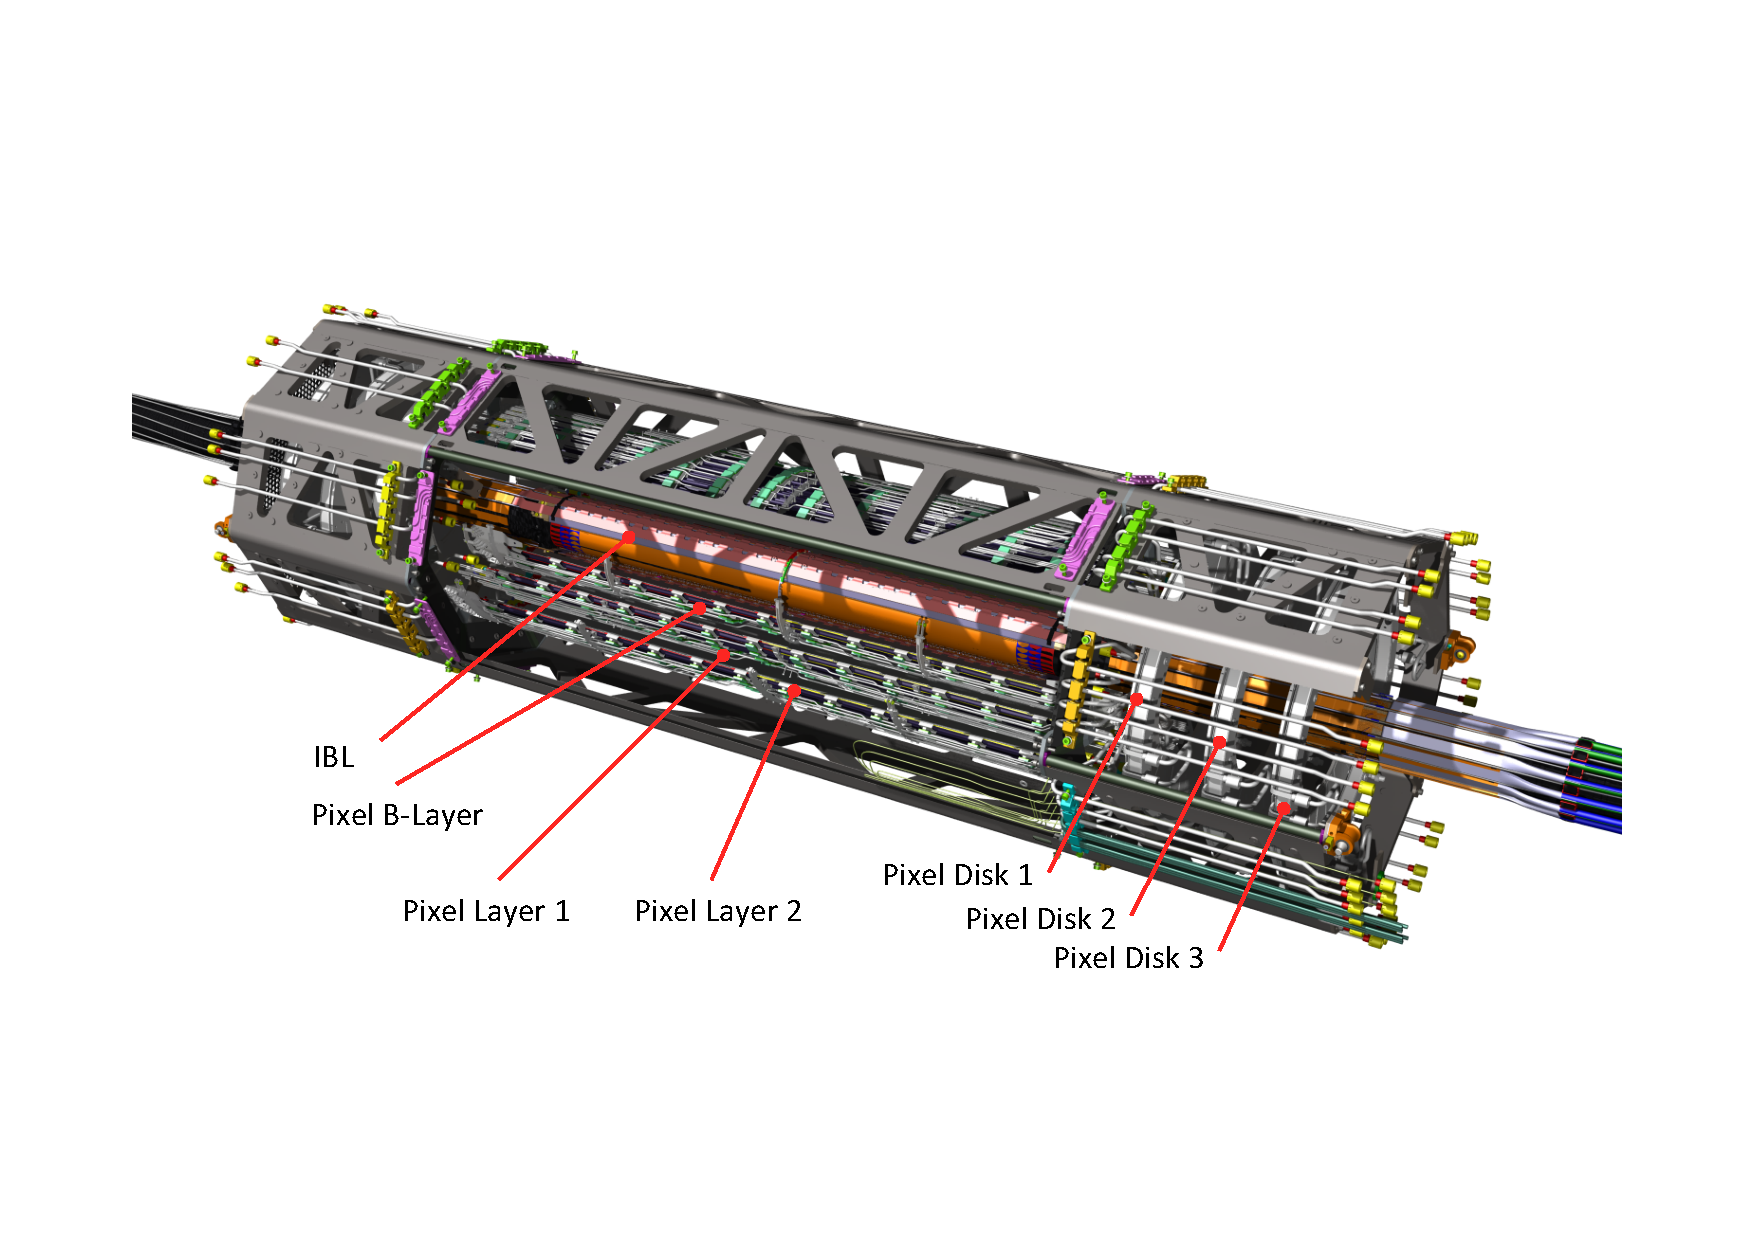
\includegraphics[width=0.8\textwidth]{Images/ibl_paper/chapter02_Physics/Pixel_IBL_rendering.pdf}
%\caption{View of the IBL detector as positioned in the Pixel detector.}
%\label{fig:IBLView1}
%\end{center}
%\end{figure}

%\begin{figure}[!htb]
%\begin{center}
%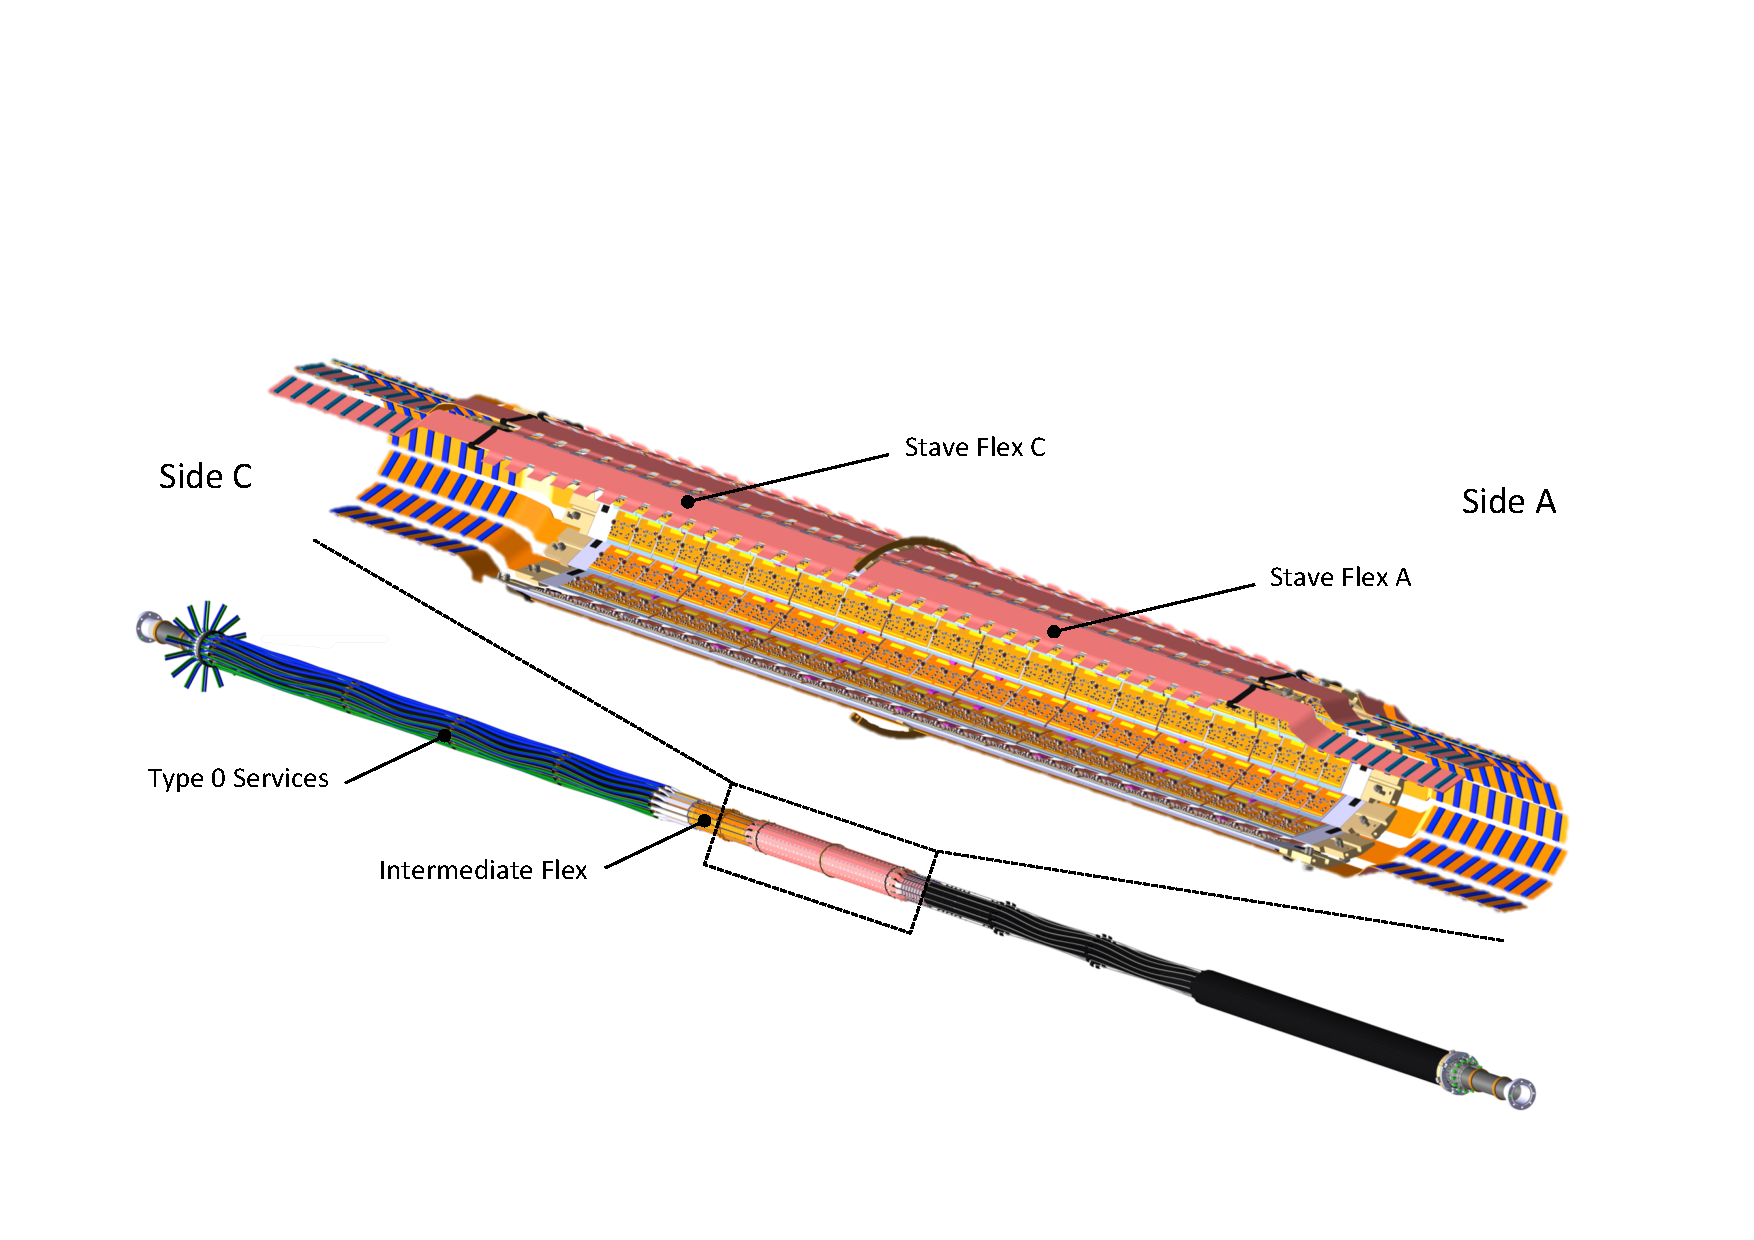
\includegraphics[width=0.8\textwidth]{Images/ibl_paper/chapter02_Physics/IBL_rendering.pdf}
%\caption{Longitudinal view of the IBL detector and its services. 
%The insert shows an enlarged view of the detector with its modules arranged cylindrically around the beam pipe.}
%\label{fig:IBLView2}
%\end{center}
%\end{figure}

\begin{figure}
\begin{center}
 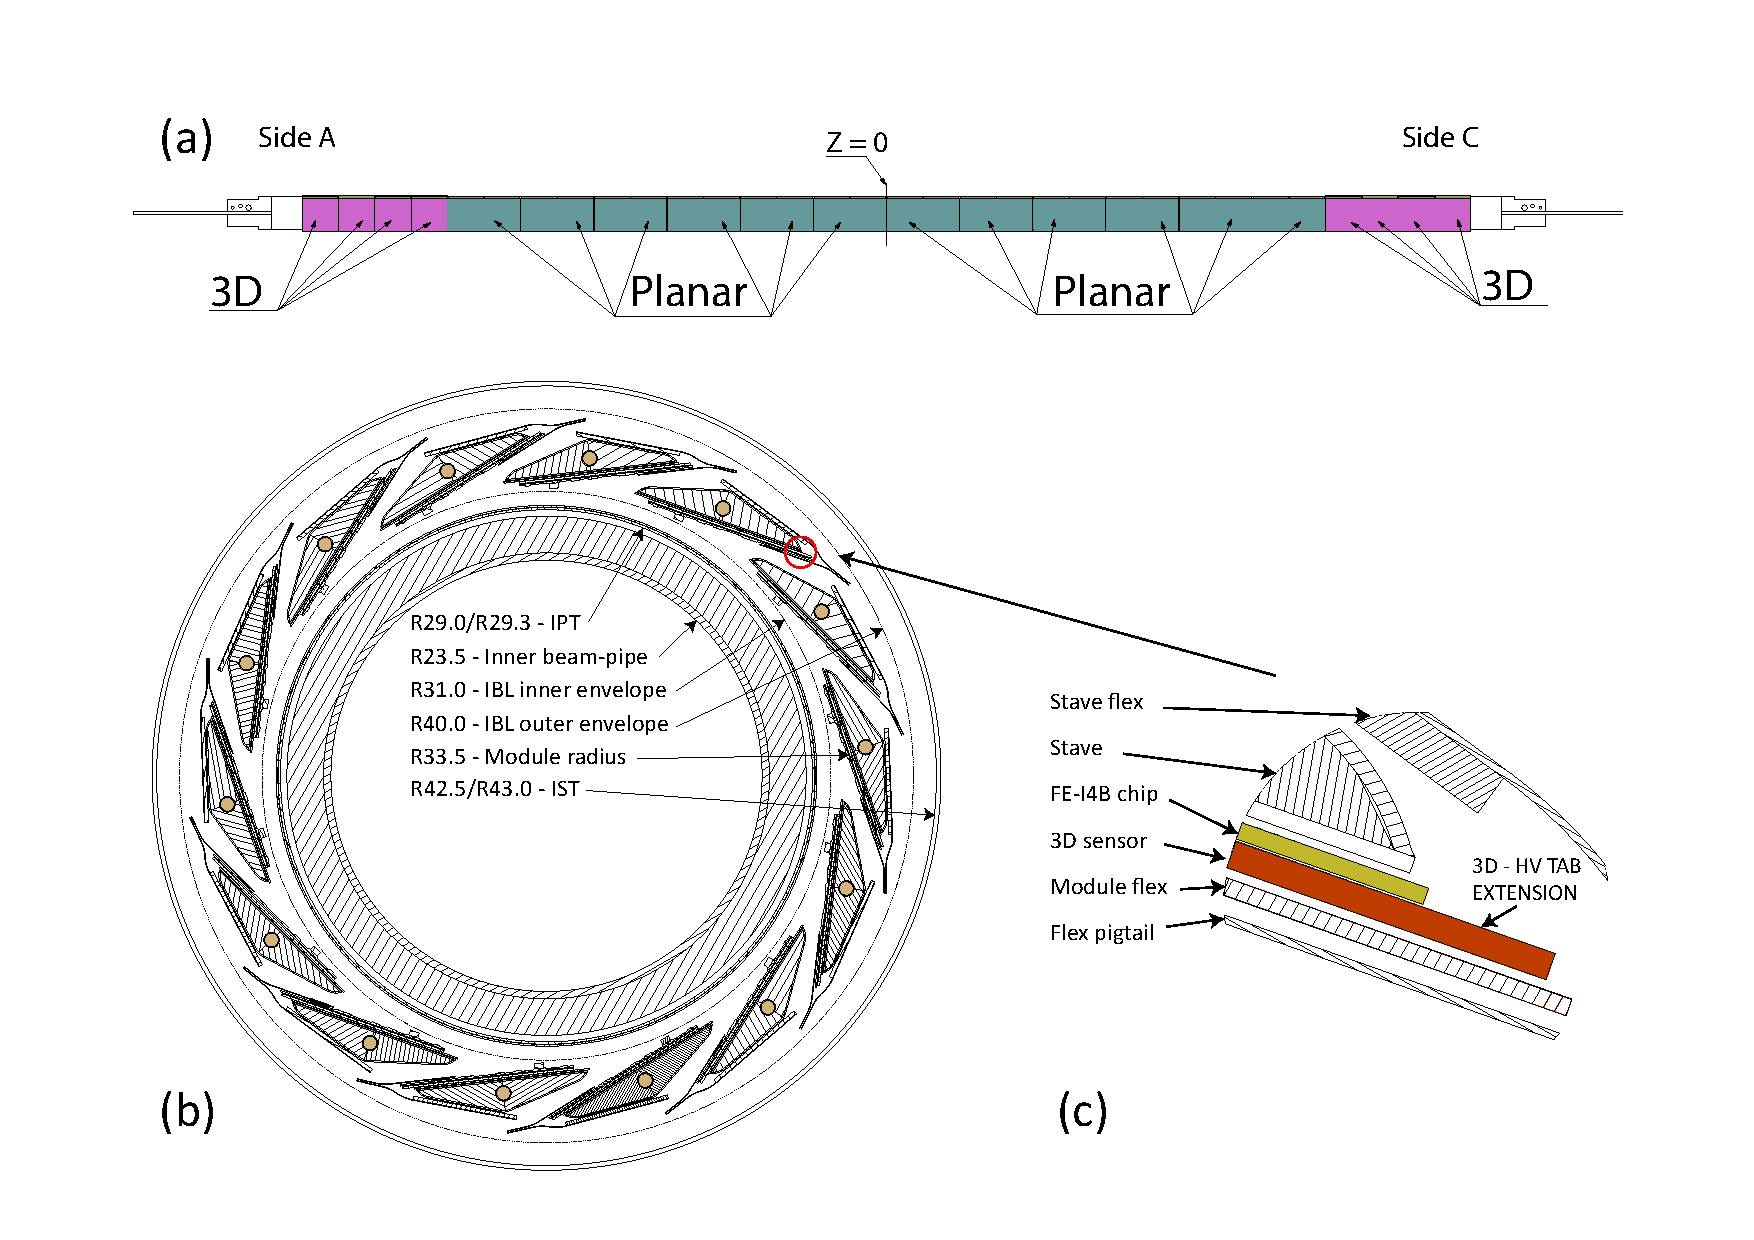
\includegraphics[width=0.8\textwidth]{Images/ibl_paper/chapter03_Overview/IBL_Layout.pdf}
\caption{ IBL layout: (a) Longitudinal layout of Planar and 3D modules on a stave. (b) An $r-\phi$
               section showing the beam pipe, the IPT, the staves of the IBL detector and the IST.
               (c) An exploded $r-\phi$ view of the corner of a 3D module fixed to the stave. }
\label{fig:IBLLayout}
\end{center}
\end{figure}
The most important layout parameters of the IBL detector are listed in Table~\ref{tab:LayoutTable} and a picture of the layout is shown in Figure~\ref{fig:IBLLayout}. The detector consists of 14 mechanical support (staves) equipped with pixel silicon modules surrounding the beam pipe, providing full azimuthal ($\phi$) coverage for high transverse momentum particles. %The nominal layer radius, i.e. the distance from the beam axis to the sensor center-of-mass, is \SI{33.5}{\milli\meter}.
Each stave hosts the electrical and cooling services to 20 pixel modules that are attached to the stave and provide a $|\eta|$ coverage up to 3. Two module types~\cite{IBL_mod_proto} are installed on each stave based on two different silicon sensor technologies: Planar and 3D. Planar sensors populate the central stave region, while 3D sensors the side region, as shown in Figure~\ref{fig:IBLLayout}. The forward region of the staves are populated by 3D sensors where they can guarantee a better z-resolution in the tracking reconstruction after heavy irradiation due to the electrode orientation. The details about the sensors are given in Section~\ref{sec:mod_sensor}. % A total of 12 Planar n-in-n sensors, similar to the present Pixel detector, each bump-bonded to  two FE-I4 readout chips, populate the central stave region. Four 3D sensors, for the first time in a particle physics tracking detector, each bump-bonded to one FE-I4 chip, populate each end of the stave. The staves  are mounted with the sensors facing the beam pipe. 
The staves are inclined by \SI{14}{\degree} with respect to the radial direction in order to achieve an overlap of the active area between staves. This tilt also compensates for the Lorentz angle of drifting charges in the case of Planar sensors, and the effect of partial column inefficiency for normal incidence tracks in the case of 3D sensors. Due to space constraints, the sensors are not shingled along the stave (in $z$). However to minimize the dead region, modules are glued on the stave with a physical gap of \SI{200}{\micro\meter}.\\
%In the End of Stave (EoS) region the detector services are connected to extensions that reach the Inner Detector End-Plate (PP1) where the connections to the external and fixed services are made after installation in ATLAS. At PP0 the cooling pipe of the stave is attached at each end to \SI{3}{\meter} length pipes. Also at PP0, the internal (Type 0) electrical services, providing data transmission and power to the modules, are connected to $\sim$\SI{3}{\meter} in length (Type I) electrical services.
A comparison between the IBL technical characteristics and the 3 layer Pixel Detector is reported in Table~\ref{tab:TableComparison}.

\begin{table}
	\centering
	\begin{tabular}{lcc}
	\hline \hline
	 & Pixel & IBL \\
	\hline
Active Surface (\SI{}{\meter\squared}) &  1.73 &  0.15 \\
Number of channels (x 10$^{6}$) & 80.36 & 12.04 \\
	\hline
	Pixel size (\SI{}{\micro\meter\squared}) & 50$\times$400 & 50$\times$250 \\
	Pixel array (FE-I4 chip) & 18$\times$160 & 80$\times$336 \\
	Chip size (\SI{}{\milli\meter\squared}) & 7.6$\times$10.8 & 20.2$\times$19.0 \\
	Active Fraction (\SI{}{\percent}) & 74 & 89 \\
	Analog current (\SI{}{\micro\ampere\per\pixel}) & 26 & 10 \\
	Digital current (\SI{}{\micro\ampere\per\pixel}) & 17 & 10 \\
	Analog voltage (\SI{}{\volt}) & 1.6 & 1.4 \\
	Digital voltage (\SI{}{\volt}) & 2.0 & 1.2 \\
	Data out transmission (\SI{}{\mega\bit\per\second}) & 40 & 160 \\
	\hline
Sensor type & Planar & Planar / 3D \\
Sensor thickness  (\SI{}{\micro\meter}) & 250 & 200 / 230 \\
Layer thickness  (\SI{}{\xzero})  & 2.8  & 1.9  \\
Cooling fluid & C$_3$ F$_8$ & CO$_2$  \\
\hline \hline
	\end{tabular}
	\caption{Comparison of the main characteristics of the Pixel detector and the IBL detector.}
	\label{tab:TableComparison}
\end{table}

The IBL volume, which contains  the staves and the services, is the space between an external Inner Support Tube (IST) fixed on the Pixel structure and a precision mechanical support called the Inner Positioning Tube (IPT). The central part of the ATLAS beam pipe is slid into the IPT tube and attached to it.
A key feature of this design approach is that independent volumes are generated and the fast removal of either the beam pipe with respect to the IBL package, or the IBL and beam pipe with respect to the Pixel package, are allowed. 
As the Pixel Detector was on the surface during 2014 for repair and service refurbishment, the IST was inserted there.
The IBL package, including the beam pipe, was then slid inside the IST once the Pixel detector was integrated and fully connected in the cavern.\\
The reduction of the material budget leads to an optimization of the tracking performance.
The averaged over $\phi$ IBL radiation length is 1.9 X$_0$ for normal incidence tracks  at $z = 0$ and it corresponds to $\sim$ \SI{70}{\percent}  of that for the Pixel B-Layer\footnote{The as-built IBL radiation length has been evaluated and then confirmed  in collisions data-taking. The difference with respect to the estimate reported in the IBL TDR~\cite{Capeans:1291633} is mainly due to a reduced initial estimate of the module material and the addition of the IPT.}. 
A lower radiation length has been achieved by using a new low-mass module design, a local support structures (staves) made of low density carbon foam, the use of CO$_2$ evaporative cooling that optimizes the mass flow and the pipe size and using aluminium conductors for the electrical power services. Table~\ref{tab:MaterialBudget} reports the main contributions to the IBL material budget. Figure~\ref{fig:IBLMaterialBudget} shows the
 material traversed by a track of origin $z = 0$ as a function of $\eta$, smeared over the 
 azimuthal angle.


\begin{table}
	\centering
	\begin{tabular}{lc}
	\hline \hline
	Item & Value (\SI{}{\xzero})\\
	\hline
	Beam pipe & 0.32 \\
	IPT & 0.12 \\
	Module &  0.76 \\
	Stave   &  0.6 \\
	Services   & 0.19  \\
%	Coolant  & ?? \\
	IST   &  0.21 \\
	\hline
	 IBL total   & 1.88 \\
	\hline \hline
	\end{tabular}
	\caption{Averaged IBL material budget over the azimuthal angle $\phi$ for normal incident tracks  at $z = 0$.  The beam pipe material is excluded from the IBL total. 
	\label{tab:MaterialBudget}}
\end{table}




\begin{figure}
	\centering
	\subfloat[\label{fig:xo_linear}]{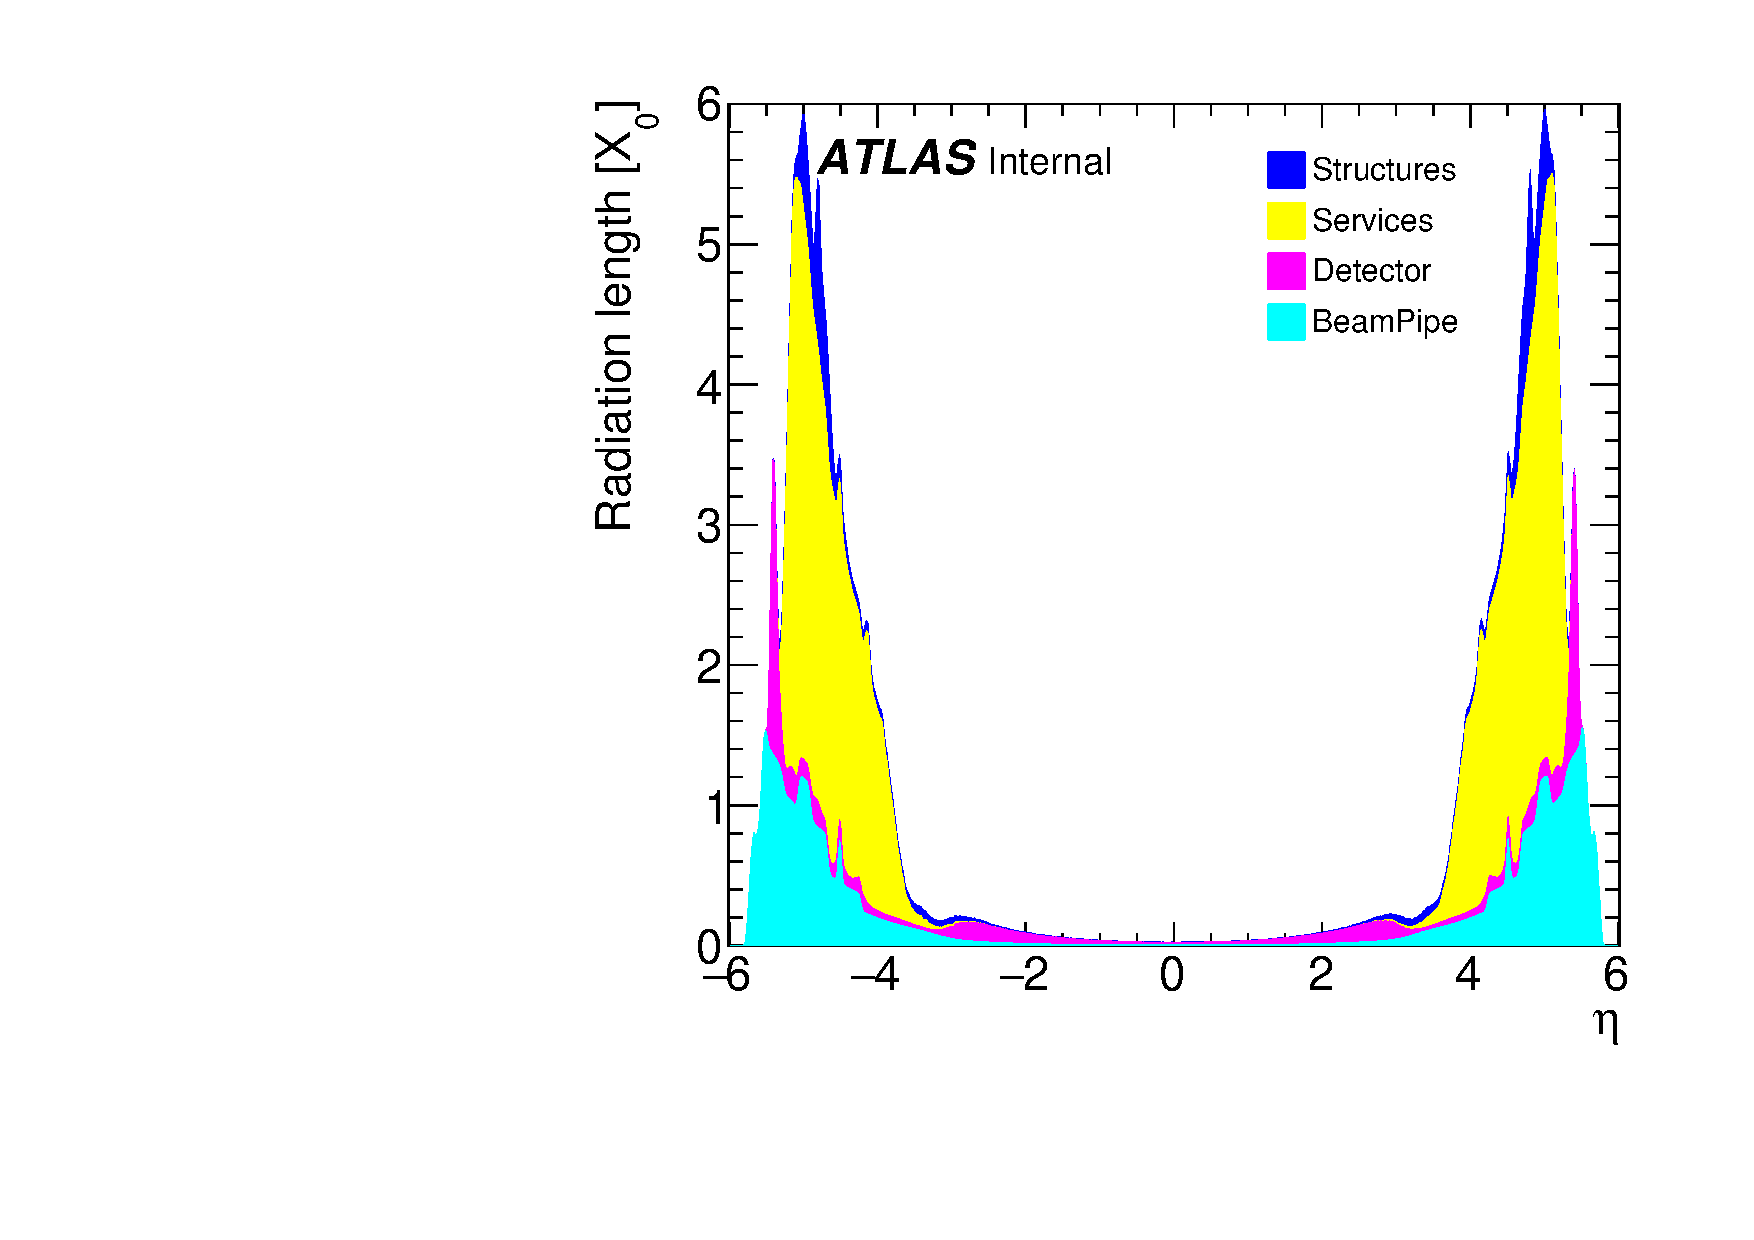
\includegraphics[width=0.47\textwidth]{Images/ibl_paper/chapter03_Overview/IBL_BP_material.pdf}}
	\subfloat[\label{fig:xo_log}]{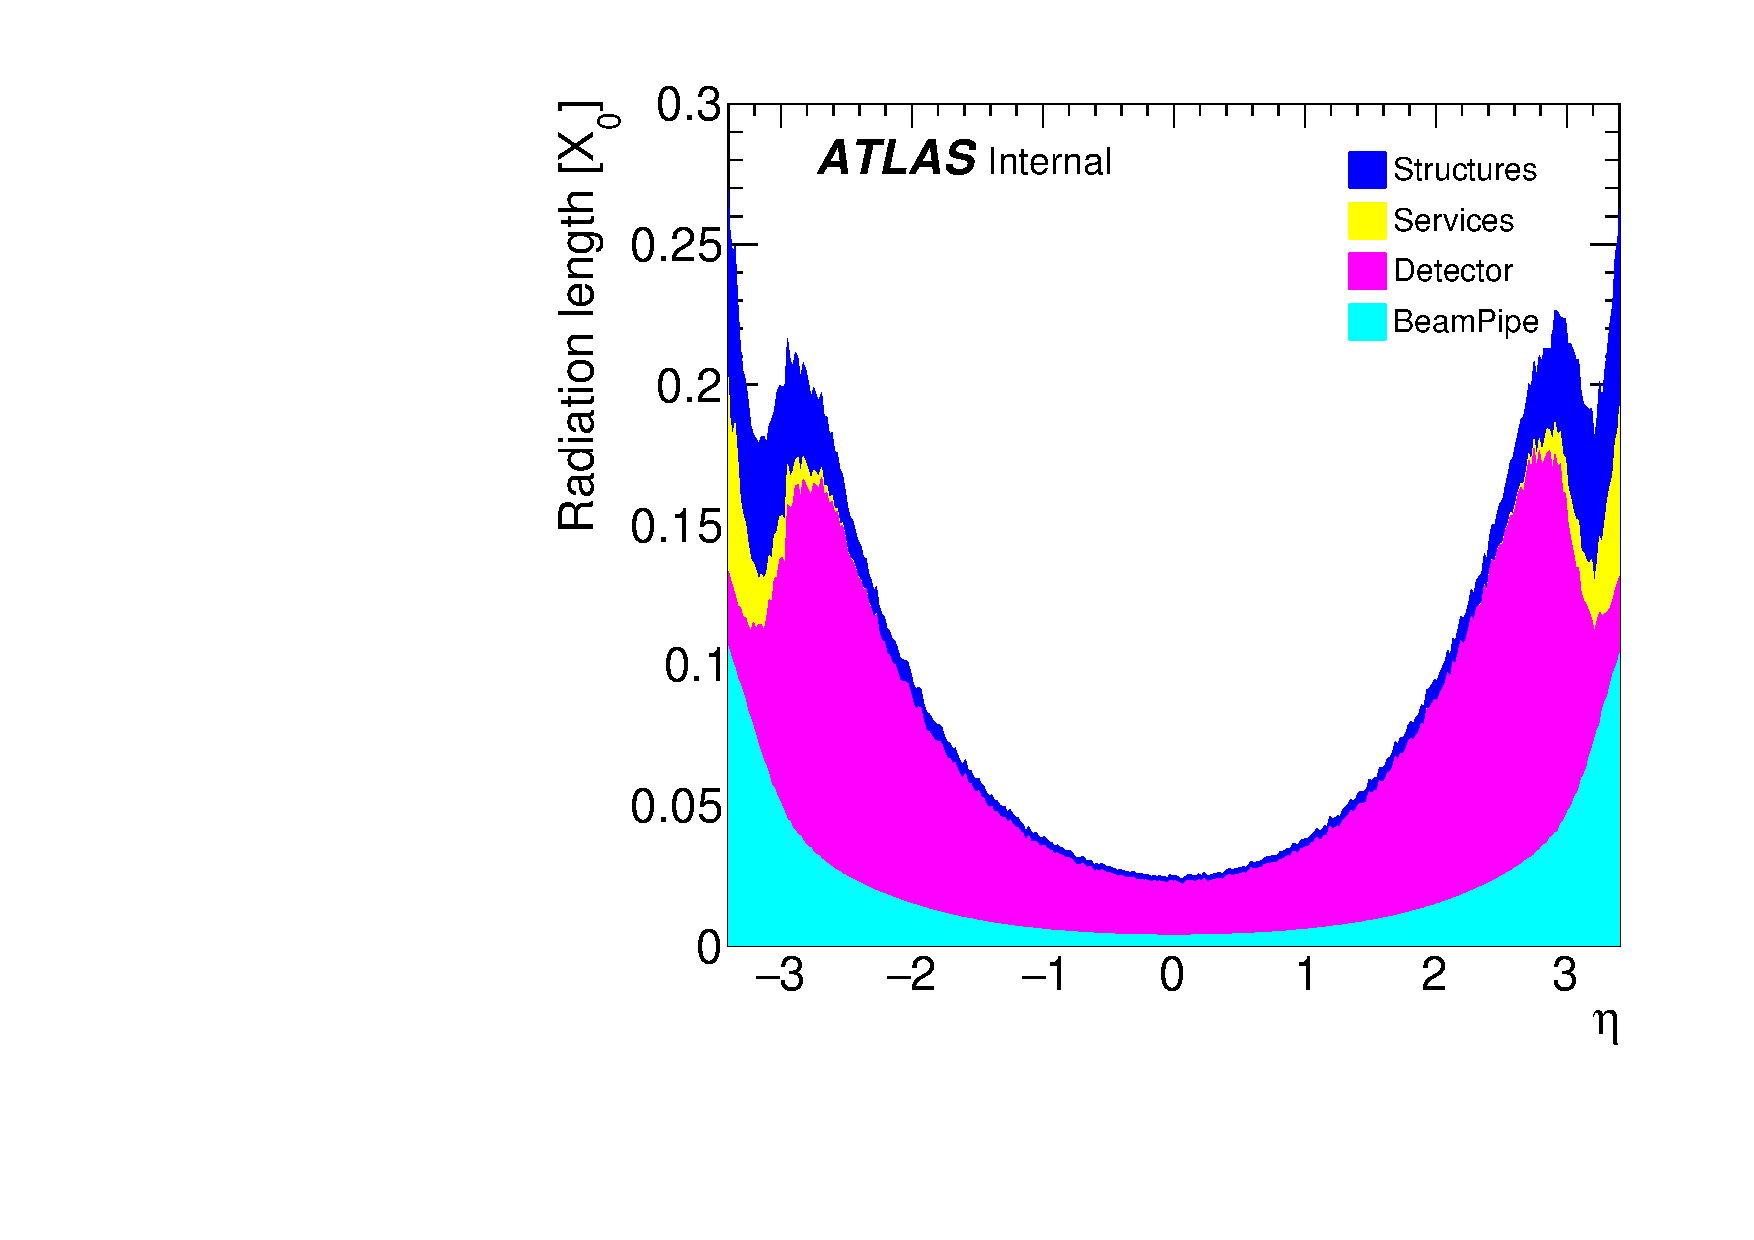
\includegraphics[width=0.47\textwidth]{Images/ibl_paper/chapter03_Overview/IBL_BP_material_zoomed.pdf}}
	\caption{(a) Radiation length as a function of $\eta$  for different components of the IBL detector as implemented in the ATLAS geometry model. Different components are shown:  the beam pipe,  the detector  (IBL staves, modules and IPT),  the services (cooling and cables) and  the structures (IST, stave rings, endblocks, sealing ring area). (b) A zoomed view of the central  $|\eta|$ distribution.}
\label{fig:IBLMaterialBudget}
\end{figure}






%\subsection{Design of IBL detector}
\subsection{Module Layout}
%\subsection{Modules}
%\label{sec:mod}

%The IBL pixel detector module is a complex entity consisting of the sensor, the FE-chip(s) and the module flex hybrid and built with many different assembly steps. Two different types of modules are used for the IBL: Double-chip (DC) modules with Planar sensors and single-chip (SC) modules with 3D sensors. In section~\ref{sec:mod_bumping}  the bump bonding process for the connection between chips and sensors is discussed. The module flex hybrid is introduced in section~\ref{sec:mod_flex} whereas the final module assembly is covered in section~\ref{sec:mod_assembly}. Details of the dressed modules are discussed in section~\ref{sec:dressed_modules} and and the results of the production QA of the dressed modules are presented in section~\ref{sec:module_qa}

The basic building block of the IBL is the module. Due to the two sensor concepts used, the IBL modules differ in size.
For Planar sensors the module consists of two FE-I4 chips connected to one sensor tile. For 3D sensors the module consist of one
FE-I4 chip connected to one sensor. A module consists of the following parts:

\begin{itemize}
\item the Planar or 3D sensor.
\item one or two FE-I4 chips each containing 26,880 pixel cells with amplifying circuitry.
\item a double-sided, flexible printed circuit (referred to as module flex).
\end{itemize}

The FE-I4 chip is described in section~\ref{sec:FEI4},  the two sensors concepts are treated in section~\ref{sec:mod_sensor} and the module flex is presented in section~\ref{sec:mod_flex}.

\subsubsection{The FE-I4 redout chip}
\label{sec:FEI4}
%The readout chip used in the first version of the Pixel detector is not capable of coping with the expected hit occupancies and radiation doses foreseen at the IBL radius, so a completely new readout chip architecture was designed.
\begin{figure}
\centering
{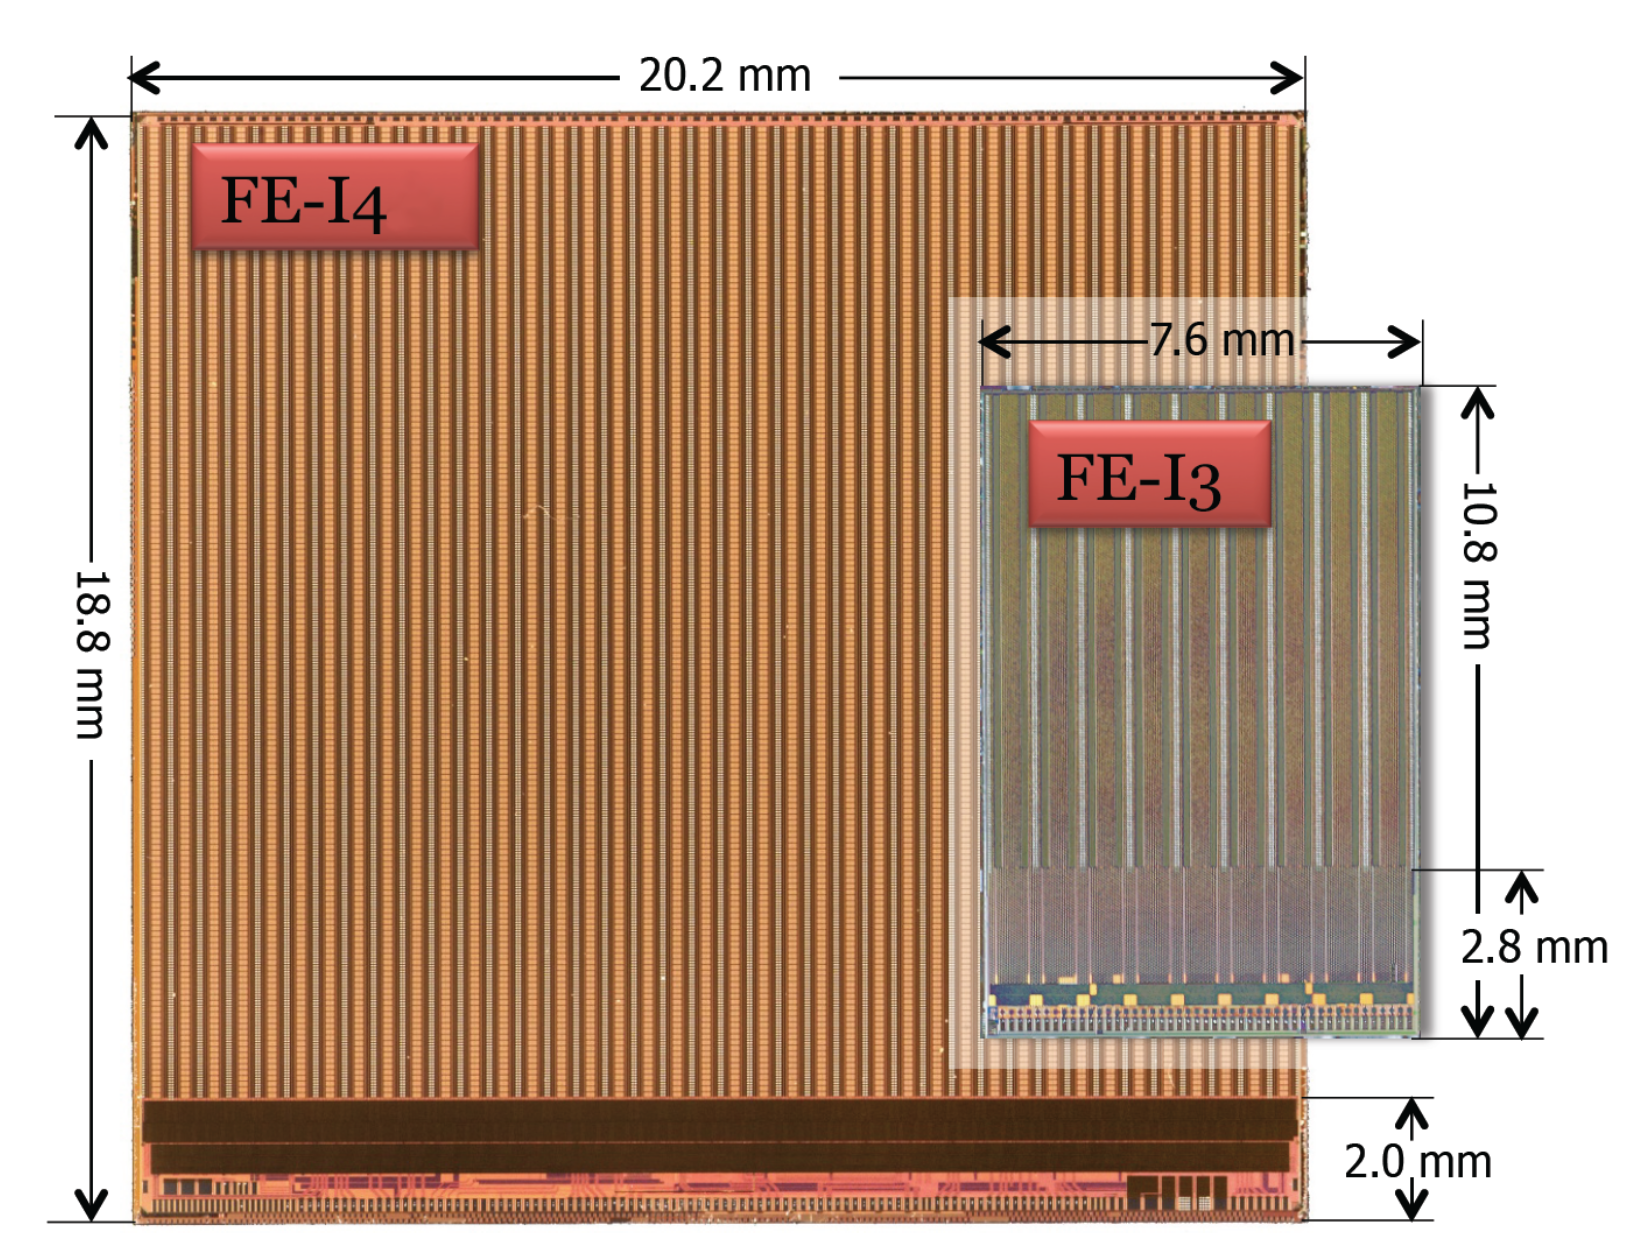
\includegraphics[width=0.5\textwidth]{Images/IBL_Paper/chapter04_Modules/FEI4.png}}
\caption{Picture of a FE-I4 chip and a to-scale picture of an FE-I3 chip. The pixel matrix and the approximately \SI{2}{\milli\meter} wide periphery can be seen.}
\label{fig:FEI4}


\end{figure}
\begin{figure}
\centering
\subfloat[Schematic view of the analog pixel cell]{\label{fig:FEI4_analog}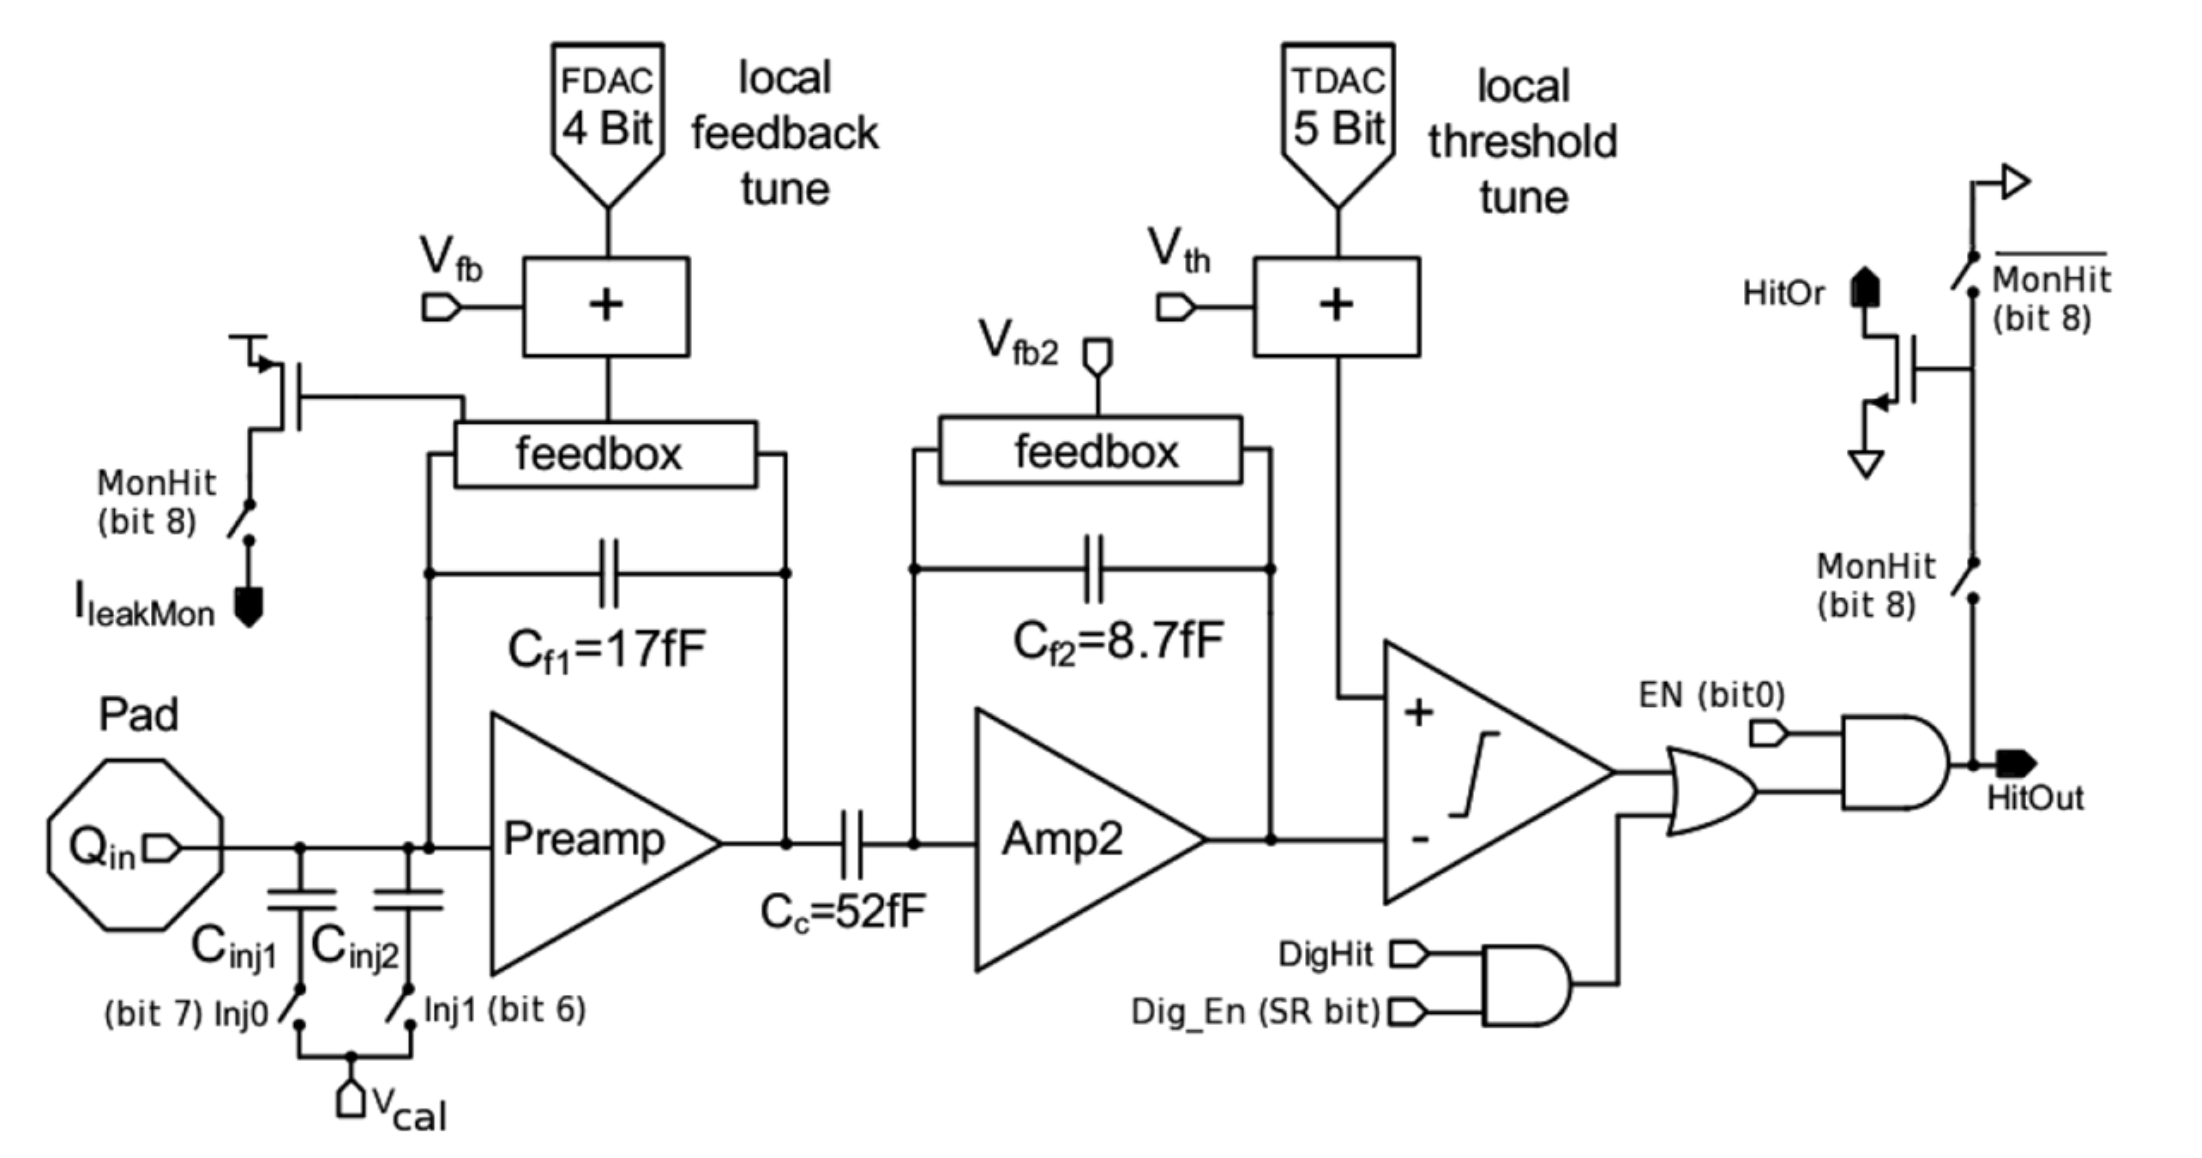
\includegraphics[width=0.8\textwidth]{Images/IBL_Paper/chapter04_Modules/FEI4_Analog.png}}
\\
\subfloat[Block diagram of the digital 4-pixel region.]{\label{fig:FEI4_digi}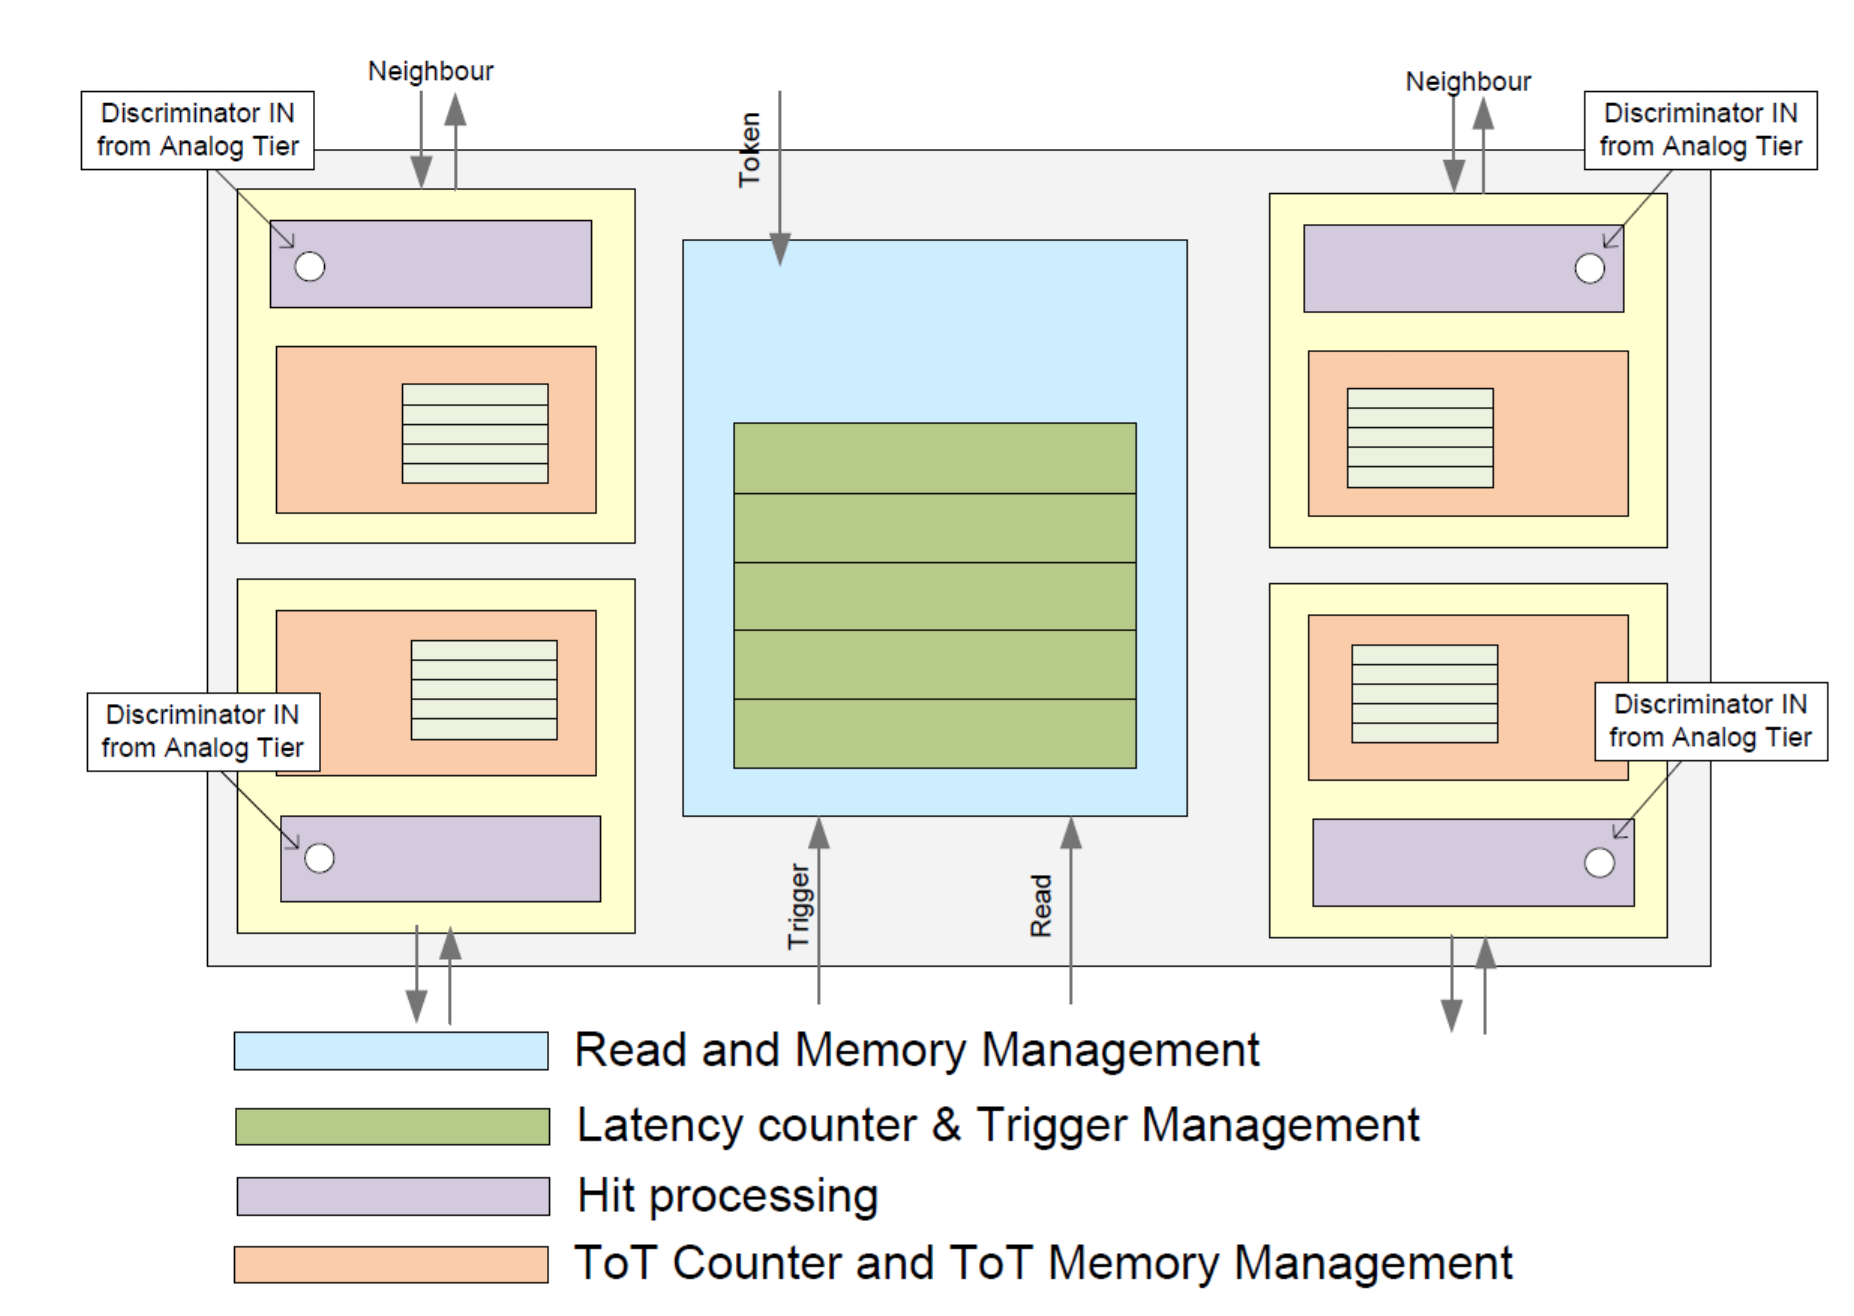
\includegraphics[width=0.8\textwidth]{Images/IBL_Paper/chapter04_Modules/FEI4_Digital.png}}
\caption{Analog and digital logic of the FE-I4 chip.}
\label{fig:FEI4_circuit}
\end{figure}
The FE-I4 is designed in a \SI{130}{\nano\meter} IBM CMOS feature size technology using thin gate oxide transistors to increase the radiation hardness. The large chip ($\SI{20.2}{\milli\meter}\times\SI{18.8}{\milli\meter}$) has an active area holding 26880 pixel, allocated in 80 columns (\SI{50}{\micro\meter} pitch) and 336 rows (\SI{250}{\micro\meter} pitch), and an approximately \SI{2}{\milli\meter} wide periphery, as shown in figure~\ref{fig:FEI4}.\\
One of the main advantage of the FE-I4 chip with respect to the FE-I3 is the lower power consumption, as it is shown in Table~\ref{tab:TableComparison}. The design of the analog and of the digital circuitry was optimized with a power consumption per pixel of \SI{26}{\micro\watt}, while it is \SI{75}{\micro\watt} for the FE-I3.\\
The analog part is a two stage charge sensitive amplifier plus discriminator design as shown in Figure~\ref{fig:FEI4_circuit}(a). The basic working principle of the two is described in Chapter 2.\\
A two-stage amplifier configuration is used, the first stage (Preamp) is a cascode amplifier while the second stage (Amp2) is a folded cascode AC coupled to the Preamp. The two-stage choice allows to provide enough gain before the discriminator while permitting the optimization in the choice of the preamp feedback capacitor ($C_{f1}$).
The preamplifier (Preamp) and second stage amplifier (Amp2) are AC coupled, and the feedback current of both amplifiers can be adjusted. These adjustments are implemented globally ($V_{fb}$ and $V_{fb2}$), so that all pixels of the matrix are affected simultaneously. For the preamplifier feedback an additional current adjustment using the 4-bit FDAC allows the fine tuning of the Time Over Threshold (\tot) response for each pixel individually. The output of the Amp2 is compared to a threshold voltage ($V_{th}$) by the discriminator. The Threshold voltage can again be adjusted globally as well as individually for each pixel.\\
The discriminator is built with a two-input voltage comparator and a threshold voltage generator. Signal shaping is only done by the preamp with an adjustable return to the baseline, while the second stage provides only the voltage gain, given by the ratio $\frac{C_c}{C_{f2}}$. The return to the baseline and the discriminator threshold are individually adjustable in each pixel, with dedicated local and global pixel registers. Two selectable capacitors are provided for analog calibration injection.\\
Additionally, each pixel contains test hit injection circuitries. Analog test signals are injected using a voltage step defined by the calibration voltage ($V_{cal}$) and two test charge injection capacitances ($C_{inj1/2}$), which can be selected independently.% The $V_{cal}$ parameter depends on a Pulser DAC as follow:
%\begin{equation}
%V_{cal}[V] = a[V] + b[\frac{V}{DAC}] \times PulserDAC[DAC].
%\end{equation}
Digital test hits are injected to an OR element at the output of the discriminator. The output of the analog readout chain of each pixel can be disabled using an AND connected to the discriminator output and the enable bit (EN) on each pixel. %The output (HitOut) can be connected to the HitOR bus which is routed to each pixel of the matrix using a logical OR and a pull down transistor, and this is low in case of any discriminator being above threshold. The HitOR signal at the wire bond pad is active high due to the an additional inverter in the periphery of the chip. This signal is used for test purposes and enables the selectable self trigger operation of the chip. Thanks the bus $I_{leakMon}$ can be used to measure the current that is compensated by the leakage current compensation logic implemented in the feedback circuitry of the preamplifier.
The feedback current of the preamplifier can be adjusted in function of the leakage current coming from the sensor, in order to compensate the latter after the irradiation.\\
Four pixels share a common digital logic cell for further hit processing as shown in figure~\ref{fig:FEI4_circuit}(b). The FE-I4 digital hit processing is based on the 4-pixel digital region. Detailed studies show that the transfer of the hit information to the chip periphery is the main inefficiency source at the expected IBL hit occupancy \cite{Malte_41}. The FE-I4 hit processing architecture therefore stores the hits in the pixel array close to the analog readout chain and the hits are processed only if a trigger signal is received. Detailed information on this architecture can be found in \cite{man_fei4b}. Four pixels share a set of five latency counters, while each pixel holds his own set of five \tot counters. A hit in one of the analog pixel cells allocates and starts the first unallocated latency counter to count down from the programmed latency (in units of \SI{25}{\nano\second}). The charge information belonging to this specific time stamp is stored in the buffers for all pixels connected to the 4-pixel digital region. An incoming Level-1 trigger in coincidence with the latency value of zero initiates the transfer of the hit data to the end of chip logic, and deallocates the latency counters and buffers. If no corresponding Level-1 trigger arrives, the hit information is deleted and the counter and buffers are deallocated as well.\\
Each of the readout chips holds two on-chip LDO (Low Drop Out) regulators (\cite{Malte_44} and \cite{Malte_45}) to generate the analog and digital supply voltages. These are linear regulators, which keep a constant output voltage independently of the input voltage and the load current. A minimum difference between the input voltage and the output voltage (dropout voltage) is used to achieve a high power efficiency. The on-chip LDOs are operated in partial shunt mode. This means that they are operated as usual LDO as long as the current consumption is above an adjustable minimum input current. If below, an additional current is shunted to ground by the regulators. This operation mode does not increase the power consumption of the FE-I4 chip as long as its current consumption in working conditions is above the shunt current. The advantage of this mode is the reduction of the transients in comparison to the pure LDO mode in case of load current fluctuations. This will happen in case of configuration of the FE-I4 or accidental configuration loss. The reference voltages needed for the operation of the two LDOs are generated on-chip.

\subsubsection{Sensors}
\label{sec:mod_sensor}

% added by sebastian

\begin{figure}
\subfloat[\label{fig:planar_collection}]{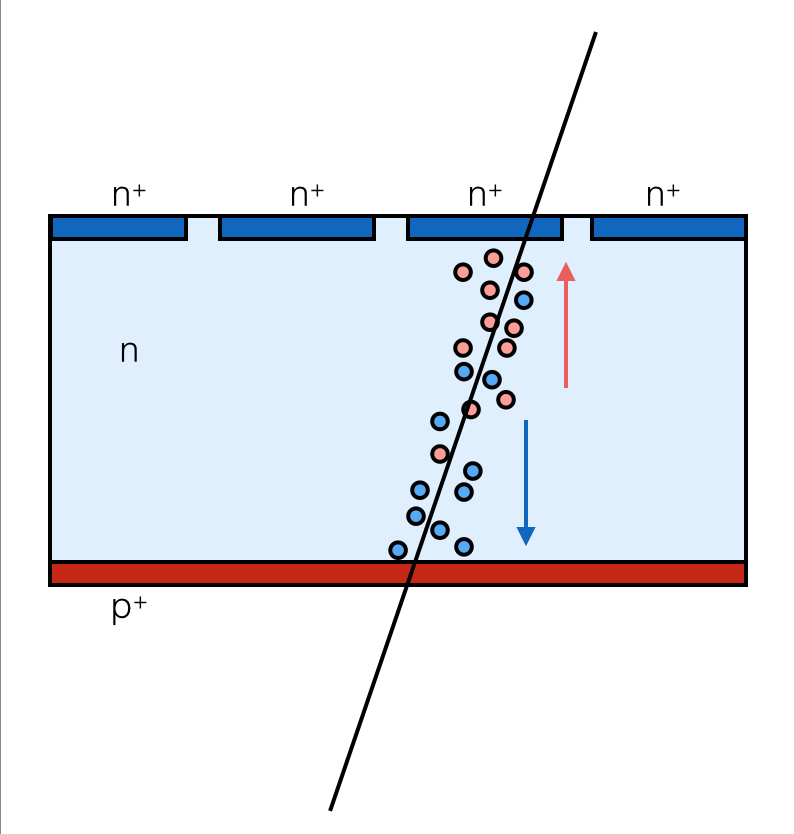
\includegraphics[width=0.48\textwidth]{Images/IBL_paper/chapter04_Modules/planar_principle.png}}
\subfloat[\label{fig:3d_collection}]{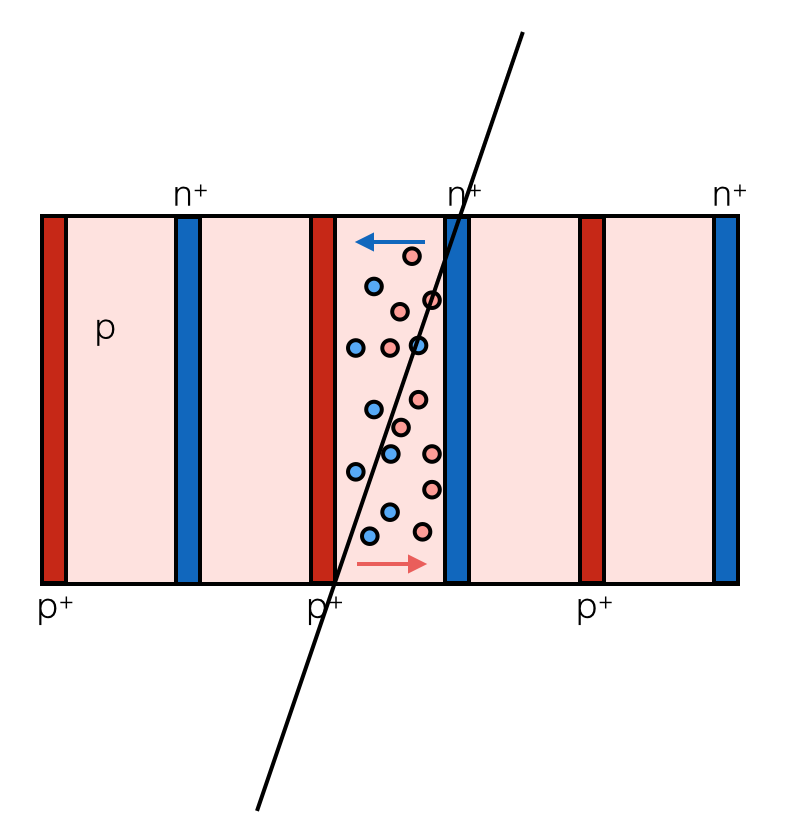
\includegraphics[width=0.48\textwidth]{Images/IBL_paper/chapter04_Modules/3d_principle.png}}
\caption{Charge collection mechanism in Planar (a) and 3D sensors (b)}
\end{figure}
Two sensor technologies are used in the IBL detector: the first is a improved version of the one used in the other layer of Pixel Detector, the Planar\cite{Planar} architecture, and a novel technology, the 3D\cite{3d} technology.
In the Planar technology the electrode are obtained on the surfaces of the bulk, the equipotential line are then parallel to the surface of the device. When the sensor is biased and a charge particle cross it, the holes and the electrons created by ionization drift towards the electrodes, moving across the bulk width as shown in Figure~\ref{fig:planar_collection}.\\
\begin{figure}[h]
	\centering
	 (a)~\includegraphics[width=0.95\textwidth]{./Images/ibl_paper/chapter04_Modules/Planar-edge-apix.png}\\
 	 (b)~\includegraphics[width=0.95\textwidth]{./Images/ibl_paper/chapter04_Modules/Planar-edge-ibl.png}\\
  \caption{Comparison of the edge designs of the (a) ATLAS pixel sensor and (b) Planar IBL pixel sensor. The inactive edge has been reduced from \SI{1100}{\micro\meter} to \SI{200}{\micro\meter}. In the guard-ring area cooler colours (such as blues) represent the n-implantation on the front-side of the sensor, warmer colours (such as reds) the p-implantation on the back-side. Figure is taken from Reference \cite{WittigPhd} with modifications.}
	 \label{fig:Planar-figure-edge}
\end{figure}
The design of the Planar sensor derives from the design of the sensor of the ATLAS Pixel Detector, which employs an n$^+$-in-n technology, where the n-side segmentation matches in size the front-end read-out electronics connected via bump-bonds. A guard-ring structure is placed on the p-side. To be compatible to the newly developed FE-I4 chip, the pixel dimensions have been shrunk to \SI{250}{} $\times$ \SI{50}{\square\micro\meter}.\\
A key features of the IBL Planar sensors is the slim-edge design which enlarges edge pixels opposite to the guard-rings and it is possible for n$^+$-in-n sensors thanks to the double sided process. This design decision was based on an extensive study which analyzed the efficiency of the sensor in the guard ring area \cite{Planar-slim-edge-2012}. No changes in the breakdown behavior have been observed as the voltage drops take place on the p-side.  The number of guard-rings was optimized based on a complementary study, which evaluated the breakdown behavior after partial guard-ring removal \cite{Planar-guard-ring-removal-2010}.  Compared to the original ATLAS pixel sensor the number of guard-rings has been reduced from 16 to 13.  Also the cutting edge has been shifted nearer to the guard-rings. In Figure \ref{fig:Planar-figure-edge} the improvement of the slim-edge design for the IBL sensor in comparison to the edge design of the ATLAS pixel sensor is shown. The combination of all three modifications, moving the cutting edge as safety margin, reducing the number of guard-rings and extending the edge pixels beneath the guard-rings, allows the reduction of the inactive edge from \SI{1100}{\micro\meter} for the ATLAS pixel design to approximately \SI{200}{\micro\meter} for the slim-edge IBL design~\cite{WittigPhd}.
The substrate material is float zone enriched with oxygen with a <111> bulk crystal orientation and a resistivity of \SIrange{2}{5}{\kilo\ohm\centi\meter}.
The production of Planar sensor for the IBL was done at CiS\footnote{CiS: Forschungsinstitut f\"ur Mikrosensorik GmbH, Erfurt, Germany}. All details of the sensor design can be found in~\cite{WittigPhd}.\\
The pixels of the two central columns of the double-chip sensor are extended to \SI{450}{\micro\meter} to keeps a necessary gap between the two adjacent front-end chips. The pixels at the outer edges of the sensor tile are enlarged to \SI{500}{\micro\meter} length. The nominal outer dimensions of the sensor layout are \SI{41300}{\micro\meter} $\times$ \SI{18600}{\micro\meter}.
The positions of high-voltage contact pads on the p-side matches the flex design openings to allow wire bonding to the sensor. Fiducial marks on the p-side of the sensor allow proper alignment of the modules during stave loading. Those marks are placed outside the guard-ring area within the dicing streets in the inactive area of the sensor.
Metallize scratch patterns are placed on the p-side of the IBL sensor close to the dicing street. In combination with the four identifying sensor numbers implemented in the metal mask on the n- and p-side of the sensor, this allows a unique identification of the sensor throughout the whole quality assurance, assembly and mounting processing of IBL sensors and modules. Some further details of the sensor design can be found in~\cite{WittigPhd}.\\
In the 3D technology the electrodes penetrate the bulk in depth perpendicularly to the sensor surface. The electrode shape is columnar and the depletion region grows around the columns. In this configuration the holes and electrons drift parallel to the sensors surface. The drift distance is not related to the width of the device, but only to the pitch between electrodes of different type. Since the inter-electrodes pitch is of the order of \SI{50}{\micro\meter}, the average distance that the electrons and holes travel in the silicon bulk is reduced in 3D sensors with respect to Planar. The possibility of recombination after irradiation is then reduced. Given the 3D electrodes geometry, the full depletion is reached for lower voltage than the Planar technology and this reflects in a lower power consumption. Given those characteristics the 3D geometry is a very good candidate for high radiation environment, being less demanding in terms of cooling and bias voltage. The fabrication process of 3D sensors is more complex and the production yield is lower than the Planar. 3D sensors do not need to compensare the Lorentz effect, due to the orientation of the electric field which is parallel to the magnetic field in ATLAS.
Test-beam investigations have shown that even if the overall efficiency was showing the same performance of the Planar, the region of the column was slightly inefficient. \\
\begin{figure}
\centering
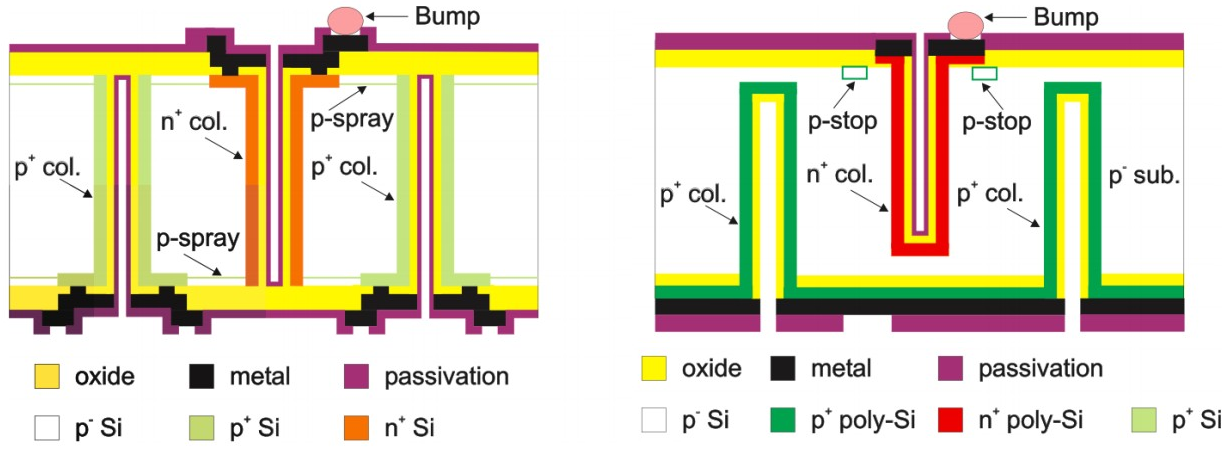
\includegraphics[width=\textwidth]{Images/ibl_paper/chapter04_Modules/3d_design.png}
\caption{\textbf{}Design of the columns of the FBK (left) and CNM (right) 3D sensors. This sketch is for illustration only and is not to scale.}
\label{fig:3d_design}
\end{figure}
In 3D pixel sensors, the column-like electrodes penetrate the substrate, instead of being implanted on the wafer surface. Thus, the depletion region grows coaxially to the columns. The $\approx\!$\SI{10}{\micro\meter} diameter columns are alternately n- and p-type doped defining the pixel configuration. The electrode spacing can be five to ten times smaller than the detector thickness (typically a few hundred microns), thereby dramatically reducing the charge-collection distance and depletion voltage. 
%The Planar technology is based on the successful design used in the Run~1 pixel detector, with several improvements. Most notably the inactive edges have been substantially reduced. The 3D sensor design~\cite{original_3d_paper} relies on column-like electrodes that penetrate the substrate, reducing the drift path with respect to the Planar approach while keeping a similar thickness and thus signal size.
%Planar sensor modules with two read-out chips cover the central region of the detector, \SI{75}{\percent} of the active area, while the forward $\eta$ regions are populated with single-chip 3D sensor modules. 
Both sensor types showed satisfactory performance in terms of noise, hit reconstruction efficiency and uniformity before and after irradiations to the fluence level of \SI{5e15}{n$_{eq}$\per\square{\centi\meter}} NIEL, as required for the operation inside the IBL~\cite{IBL_mod_proto}. 3D sensors showed an advantage in terms of power consumption due to the lower operational voltage whereas the Planar sensors proved their excellent performance during the Run~1 operation of the ATLAS pixel detector.\\ %In section~\ref{sec:Planar_design} and section~\ref{sec_3d_design} the Planar resp. 3D sensor design for the IBL is presented before in section~\ref{sec:sensor_qa} the results of the quality assurance during the sensor productions are discussed. Further performance results of both sensor types including test beam measurements are presented in detail in~\cite{IBL_mod_proto}.  
The 3D sensors for IBL have been fabricated at FBK\footnote{FBK: Fondazione Bruno Kessler, Trento, Italy} and CNM\footnote{CNM: Centro Nacional Micro-electronica, Valencia, Spain}~\cite{ds-cnm,ds-fbk}. Starting wafers were Float Zone, p-type, with \SI{100}{\milli\meter} diameter, $<100>$ crystal orientation, \SI{230}{\micro\meter} thickness, and a very high resistivity (10 to \SI{30}{\kilo\ohm\centi\meter}). Columnar electrodes, \SI{12}{\micro\meter} wide, were obtained by Deep Reactive Ion Etching (DRIE) and dopant diffusion from both wafer sides (n+ columns from the front side, p+ columns from the back side), without the presence of a support wafer. By doing so, the substrate bias can be applied from the back side, as in Planar devices. Figure~\ref{fig:3d_design} shows details of the 3D column layout.
The sensor design is detailed in~\cite{DAVIA_NIMA694_2012} and also reported in~\cite{IBL_mod_proto}. Each of the 80 $\times$ 336 pixels has a size of \SI{250}{\micro\meter} $\times$ \SI{50}{\micro\meter}, and contains two read-out (n$^+$) columns (two-electrode configuration), with an inter-electrode spacing between n$^+$ and p$^+$ columns of $\approx$\SI{67}{\micro\meter}. For yield reasons, it was decided to have single-sensor tiles (8 per wafer). A \SI{200}{\micro\meter} wide region separates the active pixel area from the physical edge of the tile. The nominal dimension of the 3D sensors are \SI{20400}{\micro\meter} $\times$ \SI{18700}{\micro\meter} (without scribe-lines).
The main differences between FBK and CNM productions are the following:
\begin{itemize}
\item FBK sensors have traversing columnar electrodes, i.e., \SI{230}{\micro\meter} deep; on the contrary, for CNM sensors, electrode etching is stopped $\approx$\SI{20}{\micro\meter} before reaching the opposite surface;
\item FBK sensors have surface isolation between n+ electrodes is obtained by a p-spray layer on both wafer sides, whereas in CNM sensors, p-stops are used on the front side only;
\item FBK sensors have the edge isolation based on a multiple ohmic column fence able to stop the lateral spread of the depletion region, whereas in CNM sensors a 3D guard-ring, surrounded by a double row of ohmic columns, is used to sink the edge leakage current.
\end{itemize}
More details on FBK and CNM 3D technologies used for the IBL production can be found in~\cite{GIACOMINI_TNS_13} and~\cite{PELLEGRINI_NIMA_13}, respectively. Table~\ref{tab:sensors} summarises the main parameters of  the IBL sensors. 



\begin{table}
\centering
\begin{tabular}{p{6cm}ccc}
\hline \hline
  % after \\: \hline or \cline{col1-col2} \cline{col3-col4} ...
\textbf{Parameter} & \textbf{Planar} & \textbf{3D CNM} & \textbf{3D FBK} \\ \hline \hline
Tile dimension [\SI{}{\micro\meter\squared}]    & 41315 $\times$ 18585 % 41315 x 18585 (nominal: 41300 x 18600)
                                                & 20450 $\times$ 18745 % 20450 x 18745 (nominal: 20400 x 18700) 
                                                & 20450 $\times$ 18745 \\
Sensor thickness [\SI{}{\micro\meter}]  & 200 & 230 & 230  \\
Pixel size (normal) [\SI{}{\micro\meter\squared}] 
                                                & 250 $\times$ 50 & 250 $\times$ 50 & 250 $\times$ 50 \\
Pixel size (tile edge) [\SI{}{\micro\meter\squared}]
						& 500 $\times$ 50 & 250 $\times$ 50 & 250 $\times$ 50 \\ 
Pixel size (tile middle) [\SI{}{\micro\meter\squared}]
						& 450 $\times$ 50 & - & - \\ 
Edge isolation       & Guard-rings & 3D guard-ring, fences & Fences \\
%Extension of efficiency for external rows [Dy @ 50% efficiency]						
Pixel isolation      & p-spray     & p-stop on n-side &	p-spray \\ \hline 
%Column depth         &             &  \SI{200}{\micro\meter}  &  \SI{230}{\micro\meter}  \\ 
%Column diameter      &             & \SI{12}{\micro\meter}  &  \SI{12}{\micro\meter}  \\						
Operating bias voltage unirradiated / \SI{5e15}{\nq}  [\SI{}{\volt}]
                                   & 80 / 1000 & 20 / 160  & 20 / 160 \\ 
 Operational power at \SI{-15}{\celsius} and after \SI{5e15}{\nq} [\SI{}{\milli\watt\per\centi\meter\squared}] 
                     &    90   
                     &    15                
                     &    15  \\ 
 \hline \hline					 
\end{tabular}
\caption{Summary of the main design specifications of Planar and 3D sensors.}
\label{tab:sensors}
\end{table}


\subsubsection{Module Flex Hybrid}
\label{sec:mod_flex}

The module flex hybrid is a double-sided, flexible printed circuit board which routes the signal and power lines between the stave flex (described later in this chapter) and the FE-chips and provides the bias voltage for the sensor via copper traces. Since both types of modules are on each stave, single-chip 3D modules and double-chip Planar modules, two types of module flexes are needed. From the layout and schematic point of view the DC module flex is a pair of two SC module flexes. The envelope of the module flex is defined by the sensor dimensions and it is slightly narrower than the sensor width. In Figure~\ref{fig:module_flexes} a picture of single-chip and double-chip module flex hybrid is shown.

\begin{figure}
\centering
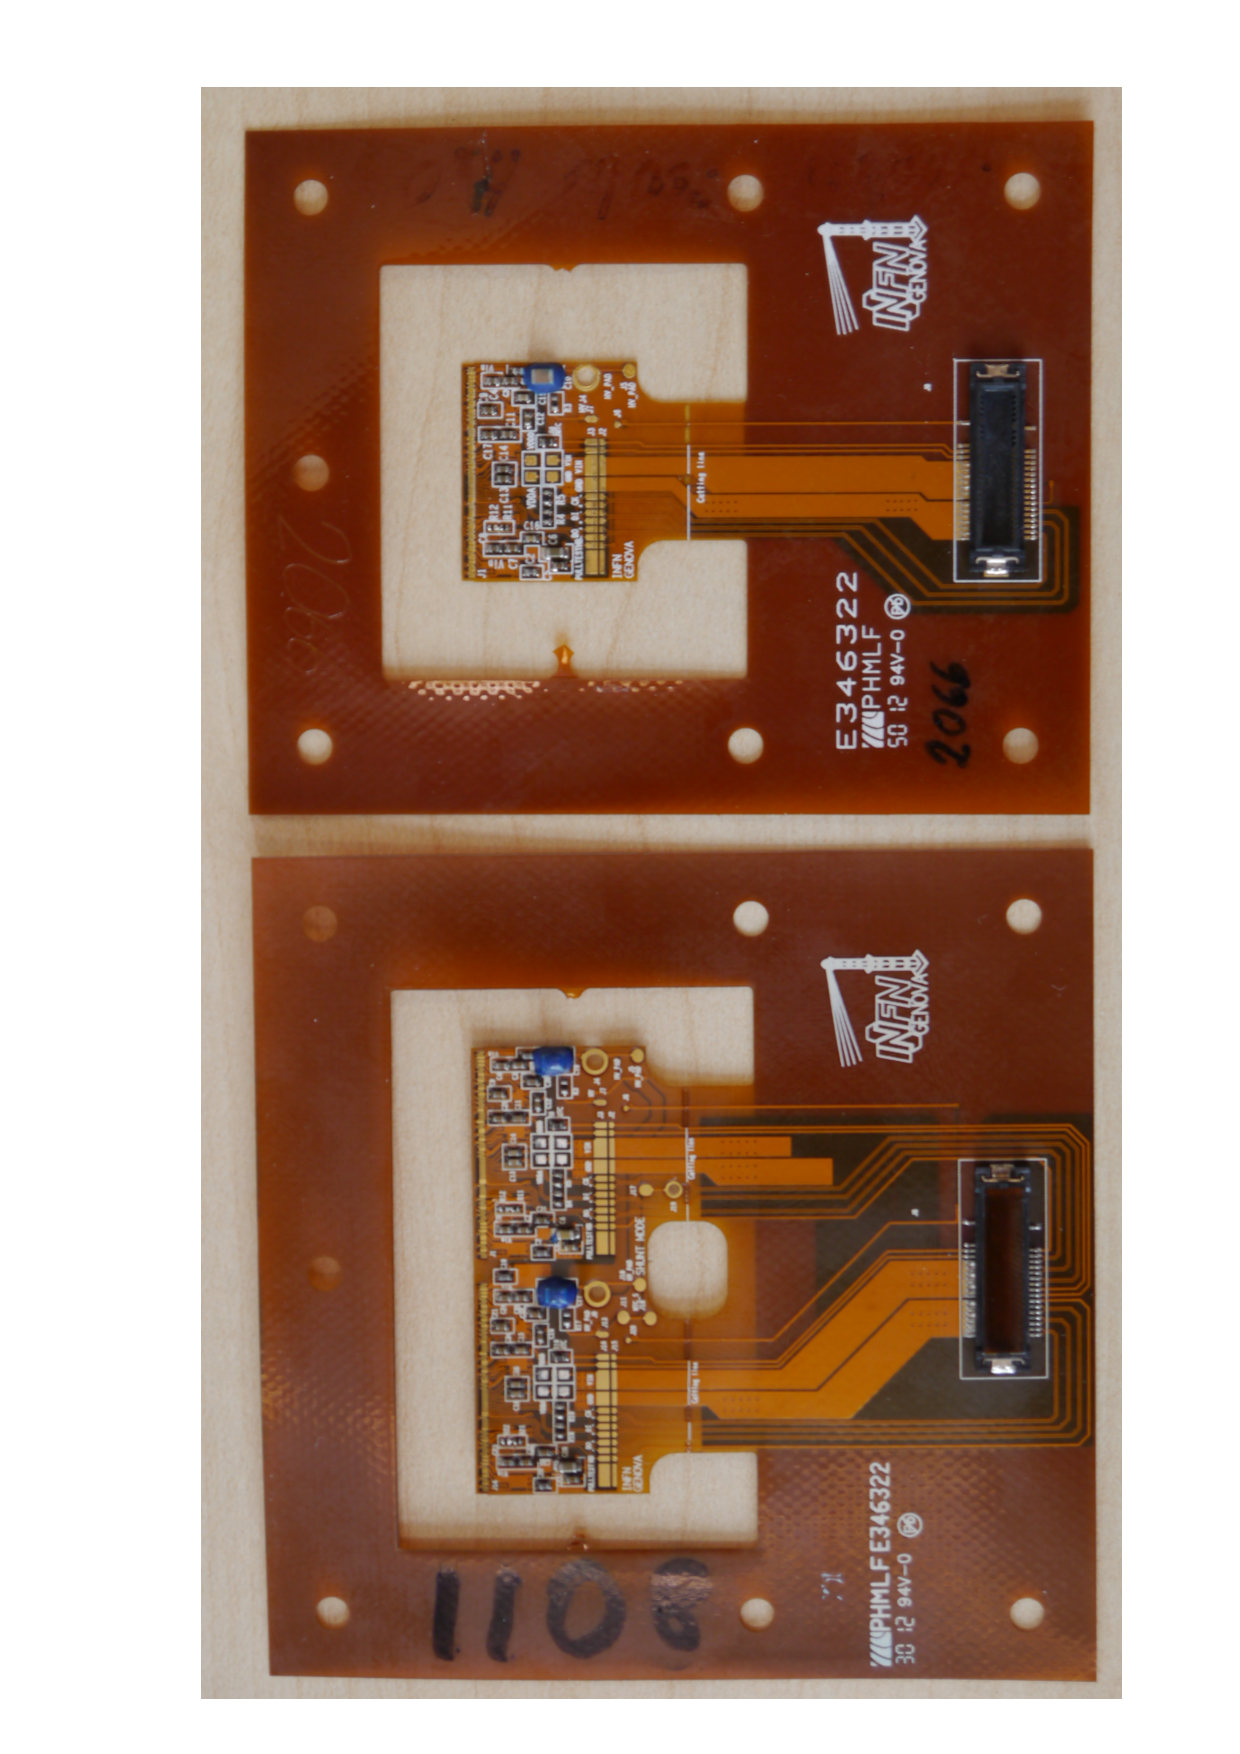
\includegraphics[width=0.4\textwidth, angle=270]{Images/ibl_paper/chapter04_Modules/module_flexes.pdf}
\caption{Photographs of a double-chip (left) and a single-chip module flex hybrid (right). The frame and flex extension allows testing of the module before loading on stave. It is cut during the stave loading procedure at a cutting line indictated as white line slightly outside the bare module envelope.}
\label{fig:module_flexes}
\end{figure}

The module flexes are glued to the sensors's backside and are connected to the longitudinal stave flex which is located at the backside of the stave via thin transversal wings, one per read-out chip. The layer stack is \SI{130}{\micro\meter} consisting of two copper layers, each \SI{18}{\micro\meter} thick, and the dielectric kapton layers, which are all glued together with acrylic adhesive layers. Passive components are mounted on the module-flex for decoupling and filtering of the read-out chips and for terminations of the signal traces. The module temperature is remotely monitored via a Negative Temperature Coefficient (NTC) thermistor added on the module-flex. All passive components are soldered on the top layer of the flex. Special emphasis is given to high voltage (HV) routing and filtering since the flex hybrid has to be functional up to \SI{1000}{\volt}. To avoid HV discharges, sufficient space between HV traces and signal and low voltage (LV) traces are introduced. The HV capacitor is encapsulated with a polyurethane resin and \SI{27}{\micro\meter} thick kapton cover layers are used on the top and bottom of the flex.

All signal and power traces of the module flex are routed to a 50-pin connector outside the module area used during production testing of the modules. Underneath the connector a stiffener is added to make the frame more rigid. Both module flex hybrid types use the same connector, and an intermediate wire bond connection is necessary to connect all signal and power lines from the flex to the connector on the frame. Prior to the loading of the module to the staves this connector area is cut away. The cutting line is about \SI{1.5}{\milli\meter} away from the sensor. The cutting area of the module flex hybrid is smaller in width than the stave flex hybrid wings to avoid any part of the residual cut area touching other components of the detector. Finally the wire bond pads for the intermediate connection are re-used to connect the modules flex hybrid to the stave flex hybrid wings using wedge bonding. 

The module flex hybrids were produced at Phoenix\footnote{Phoenix S.r.l., Via Burolo 22, 10015 Ivrea (Torino), Italy} and surface mounted device (SMD) component loading, including encapsulation, was performed at Mipot\footnote{Mipot S.p.A., Via Corona 5, 34071 Cormona, Italy}. Basic quality assurance (QA) like testing of line integrity for open and shorted connections were done by the vendors and was followed by more detailed QA tests at the two module assembly sites. These QA procedures include HV standoff tests at 1.5~kV, visual inspection and dedicated cleaning to allow for high-quality wire bonding.


\subsubsection{Dressed modules}
\label{sec:dressed_modules}
\begin{figure}
	\centering

		\subfloat[\label{fig:SC_picture}]{		 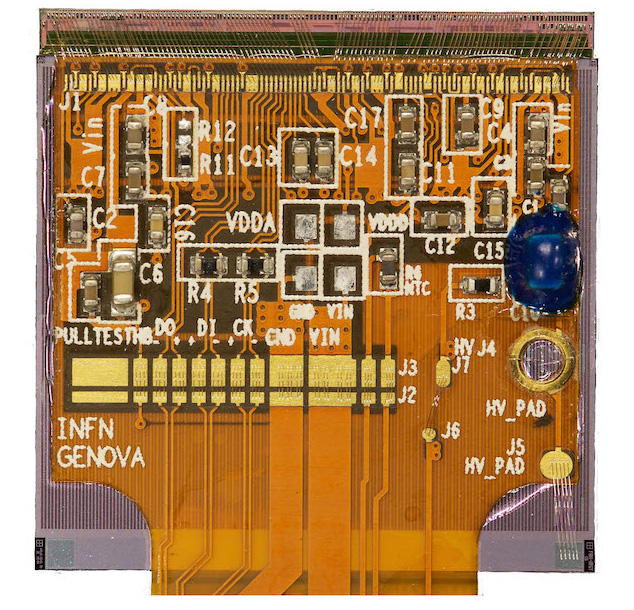
\includegraphics[width=0.335\textwidth,angle=180]{Images/ibl_paper/chapter04_Modules/IBL_module_photo_SC_HD.jpg}}
		\subfloat[\label{fig:DC_picture}]{ 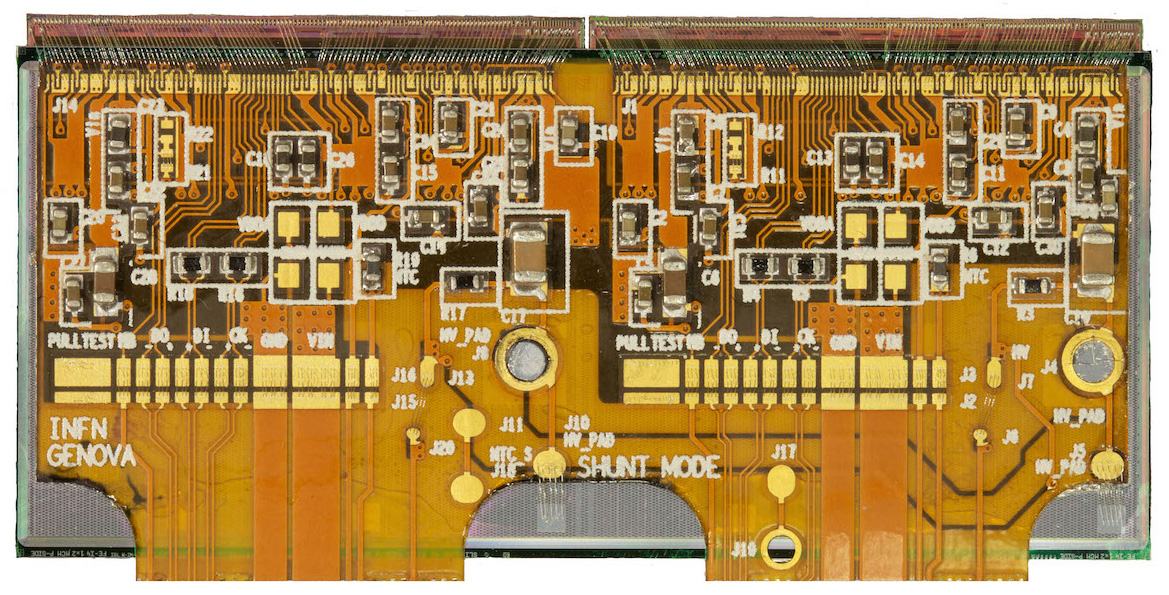
\includegraphics[width=0.655\textwidth,angle=180]{Images/ibl_paper/chapter04_Modules/IBL_module_photo_DC_HD.jpg}}
  \caption{Photographs of a dressed IBL single chip module (a) and a double chip module (b). The flex extension visible on the top allows testing of the module before loading on stave. It is cut during the stave loading procedure at a cutting line slightly above the bare module.}
	\label{fig:module_pictures}
\end{figure}
In Figure~\ref{fig:module_pictures} pictures of a fully dressed single chip and a double chip module are shown. The modules are cut out of the handling frame.
The entire design of the module is optimized for low material budget wherever possible. The FE chips are thinned to \SI{150}{\micro\meter} and the sensor thickness is reduced to \SI{200}{\micro\meter} for Planar sensors and \SI{230}{\micro\meter} for 3D sensors. The thickness of the double sided flex has been chosen to be only \SI{130}{\micro\meter} and the number of SMD components is reduced to a minimum. Table~\ref{tab:module_x0} summarizes the thickness of the IBL modules and its parts in units of the radiation length X$_0$ for perpendicular particle penetration. The contributions of the different materials are averaged over the module size. The total thickness of a Planar IBL module is \SI{0.58}{\xzero} and \SI{0.61}{\xzero} for a 3D module. 
\begin{table}
\centering
\begin{tabular}{lc}
\hline \hline
	 & \SI{}{\xzero}\\
\hline
FE chip & 0.21 \\
Planar sensor & 0.24 \\
3D sensor & 0.27 \\
Module flex incl. SMD components & 0.13 \\
\hline
Sum for Planar module & 0.58\\
Sum for 3D module &  0.61\\
\hline \hline
\end{tabular}	
\caption{Breakdown of material budget for the IBL modules in thickness in units of the radiation length.}
\label{tab:module_x0}
\end{table}


\subsection{Stave Layout}
 % Chapter coordination: Claudia, Eric

The IBL modules are supported and cooled by means of fourteen mechanical supports, the staves, cylindrically arranged around the beam-pipe. In this section a description of the support stave and of the flexible printed circuits used as services for the stave is given.


\subsubsection{The support stave}

The support stave design is motivated by several important requirements:
\begin{itemize}
\item A low radiation length to improve physics performance,
\item An excellent thermal performances to cool down silicon sensors to maximize signal to noise and to prevent thermal runaway,
\item Good mechanical stability for the most efficient tracking performances,
\item A low thermal expansion coefficient of materials to reduce stress and increase stability.
\end{itemize}

%\paragraph{Design}
As shown in Figures~\ref{fig:StaveConcept}, \ref{fig:StaveCrossSection} the stave is an assembly of four main components: the cooling pipe, the carbon foam to drain the heat flux; carbon laminates to reinforce the stave stiffness (the face plate where module will be loaded and the back stiffener on the opposite side); and the peek to assemble the stave on fixations parts around the beam-pipe. These complex materials require specific manufacturing techniques. For example: carbon laminate requires fabrication in high pressure oven to obtain the required transverse thermal conductivity; assembly process require accurate gluing for material minimization; and the titanium cooling pipes require accurate machining and minimal wall thickness (\SI{0.12}{\milli\meter} wall thickness) compatible with high pressure  CO$_2$ operation. 

\begin{figure}
\begin{center}
% 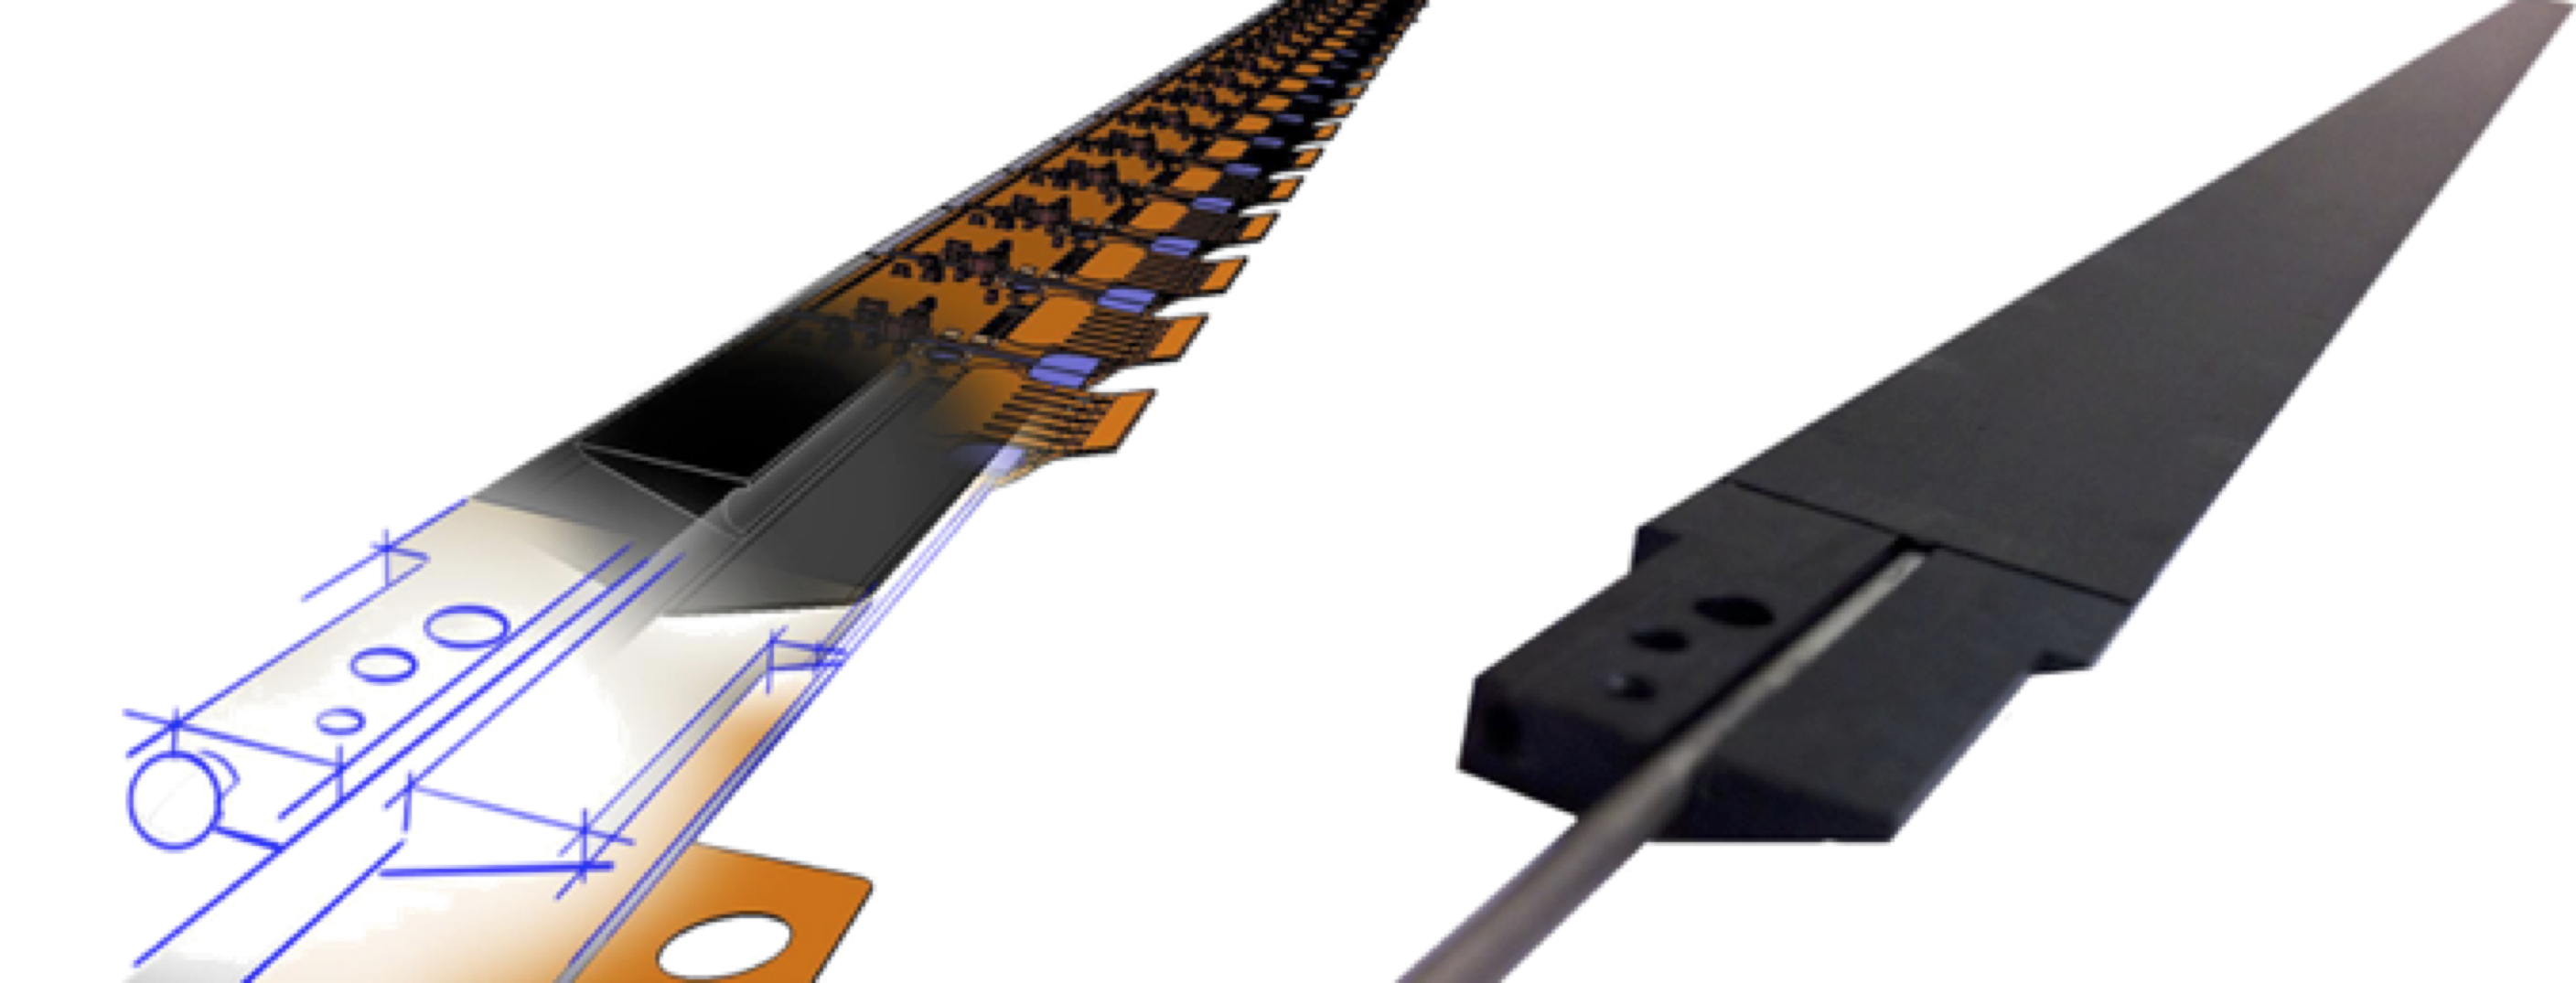
\includegraphics[width=0.8\textwidth]{Images/IBL_Paper/chapter05_Staves/StaveConcept.jpg}
 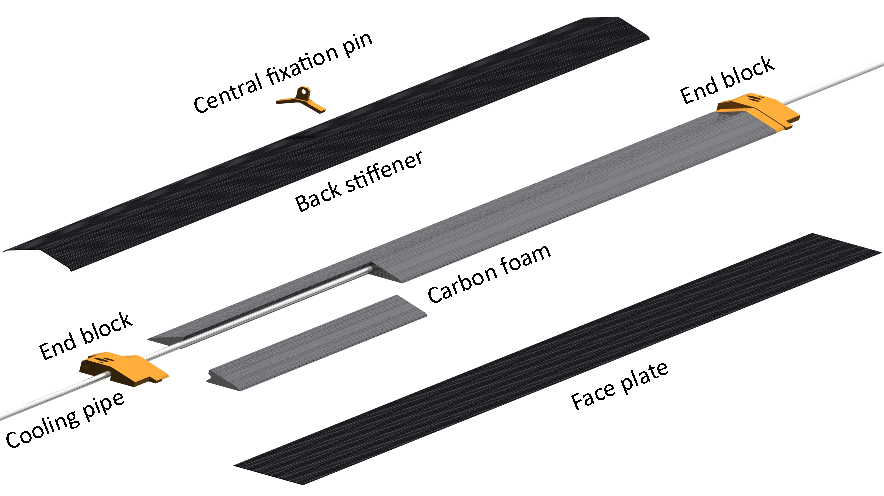
\includegraphics[width=0.8\textwidth]{Images/IBL_Paper/chapter05_Staves/BareStaveStructure_text.pdf}
\caption{Sketch of the support stave structure.}
\label{fig:StaveConcept}
\end{center}
\end{figure}

\begin{figure}
\begin{center}
 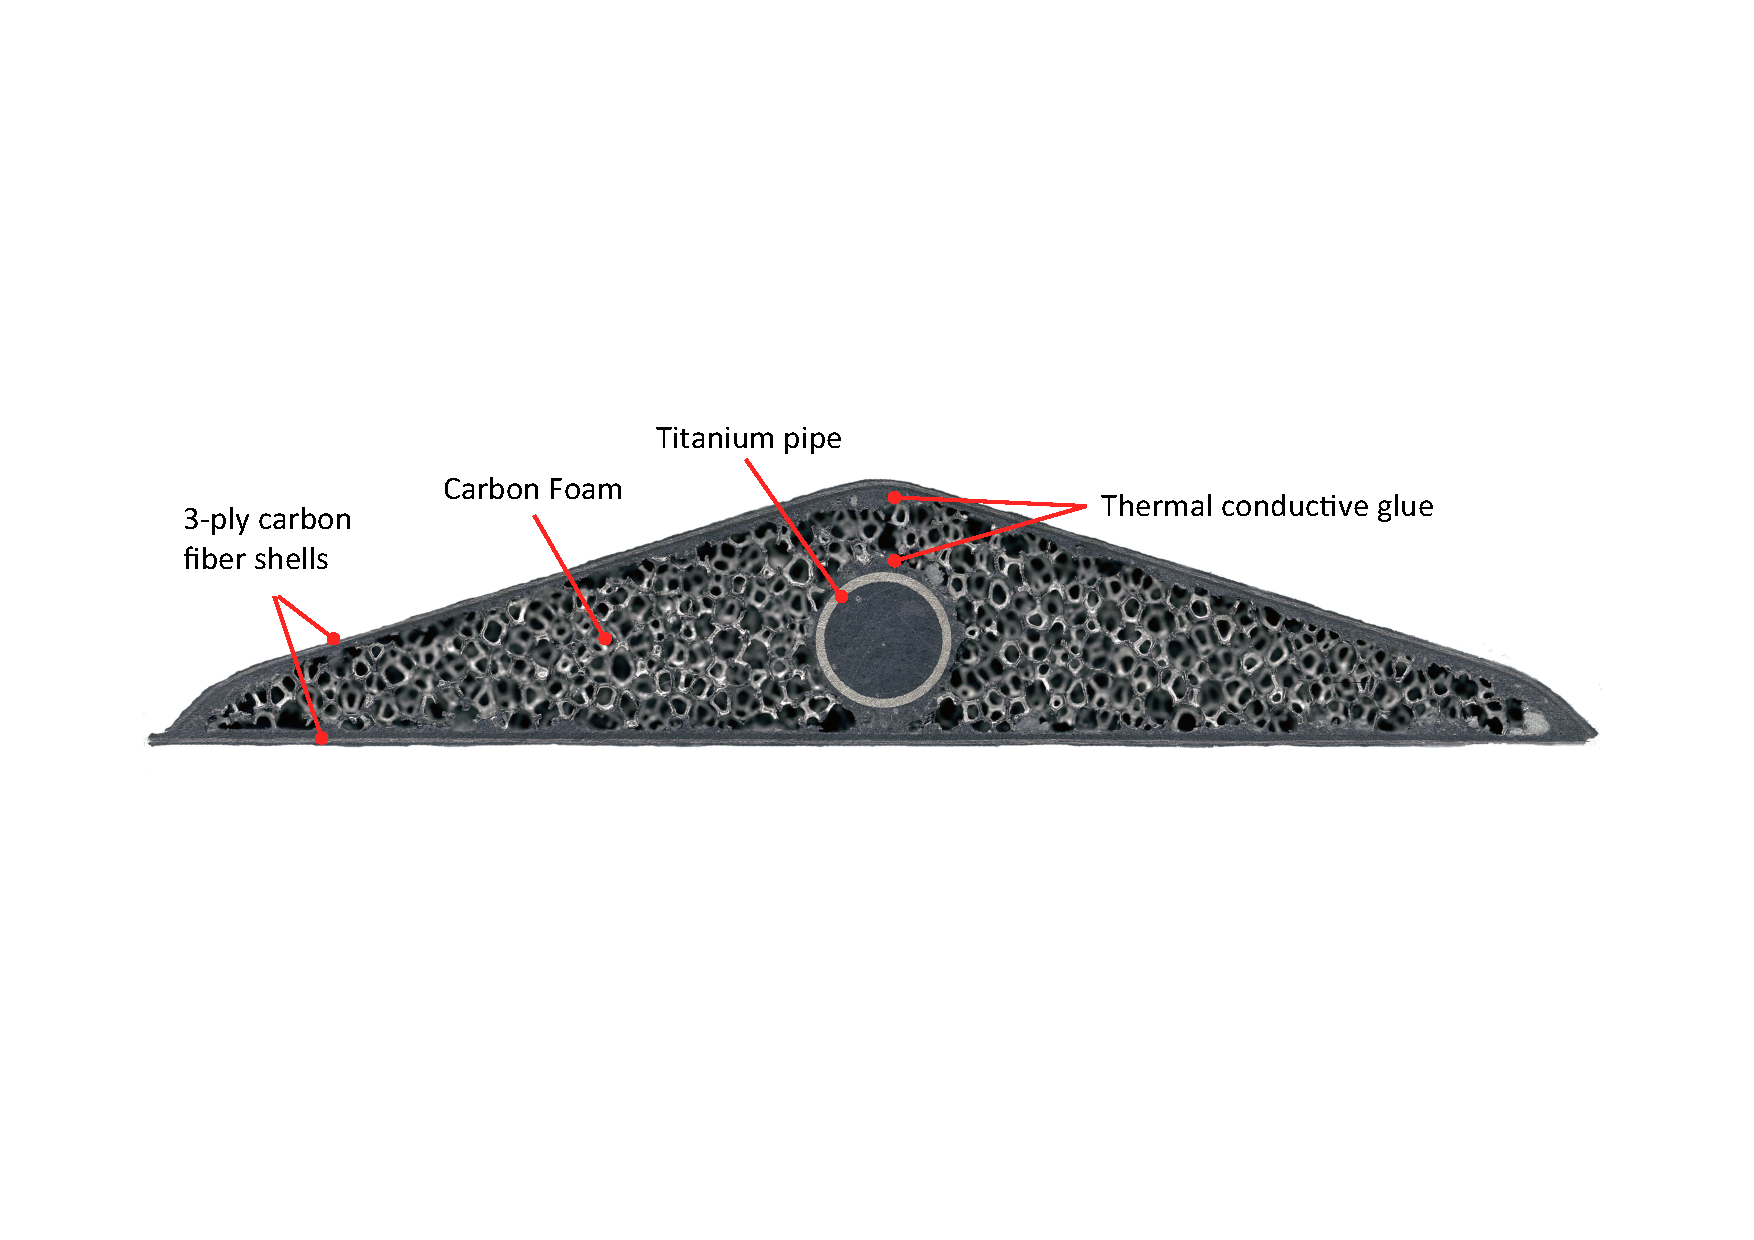
\includegraphics[width=0.8\textwidth]{Images/IBL_Paper/chapter05_Staves/Stave_section_WBG.pdf}
\caption{Stave section picture.}
\label{fig:StaveCrossSection}
\end{center}
\end{figure}

Minimizing materials is one of the most important requirements for the IBL detector to guarantee the required physics performances. For the support stave, this has led to a very aggressive design and choice of materials while maintaining a high level of reliability. The total material budget of the support stave structure is \SI{0.62}{\xzero} and the contribution of each part is  detailed in Table~\ref{tab:staveX0}. %The main properties of the used material in the support stave assembly are summarized in Table~\ref{tab:stavecomponents}.


\begin{table}
\centering
\begin{tabular}{l c c c c c }
\hline \hline
        Component & Material  & Volume/stave      & Eq. Thickness & X$_0$ & X/X$_0$  \\
                      &   &  (\SI{}{\centi\meter^3}) &             (\SI{}{\centi\meter})      & (\SI{}{\centi\meter})             & (\SI{}{\percent})      \\
\hline
% By Eric was
%Omega               &  K13C/RS3 & 2.02 & 0.144 & 21. 1 & 0.068 \\
%Glue layers & Stycast 2850FT & 3.29 & 0.234 & 8.97  &  0.2608\\
%Foam                             & K9 & 21.60 & 1.536 & 213 &   0.0721\\
%Ti pipe & Titanium T40           & 0.411 & 0.029 & 3.56 &  0.0821\\
%Face plate       &  K13C/RS3 & 1.903 & 0.135 & 21.1 & 0.0641 \\
%End of Stave fixation & Peek CA 40 & 2.51   & 0.178 & 25 &  0.0714\\
%Central fixation          & Peek CA 40 & 0.075 & 0.005 & 25 & 0.0021 \\

Back stiffener    &  K13C/RS3 & 2.02 & 0.144 & 21. 1 & 0.068 \\
Glue layers & Stycast 2850FT & 3.29 & 0.234 & 8.97  &  0.261\\
Foam                             & K9 & 21.60 & 1.536 & 213 &   0.072\\
Cooling pipe & Titanium T40           & 0.411 & 0.029 & 3.56 &  0.082\\
Face plate       &  K13C/RS3 & 1.903 & 0.0135 & 21.1 & 0.064 \\
End of Stave fixation & Peek CA 40 & 2.51   & 0.178 & 25 &  0.071\\
Central fixation          & Peek CA 40 & 0.075 & 0.005 & 25 & 0.002 \\
\hline
Total:              &  &  &  &  & 0.621 \\
\hline \hline
\end{tabular}   
\caption{Support stave radiation length budget.  %\textit{\bf Check digits!}
\label{tab:staveX0}}
\end{table}


%\begin{table}
%\centering
%\begin{tabular}{l c c c c c c }
%\hline \hline
%        Component & Density  & K      & CTE@\SI{20}{\celsius} & Young Mod. & Tensil  & Compressive  \\
%                     &  (\SI{}{\gram\centi\meter\squared})    & (\SI{}{\watt\per\milli\kelvin}) &       (\SI{}{\micro\meter\per\milli\celsius})            & (\SI{}{\giga\pascal})             & Strength (\SI{}{\mega\pascal})                & Strength  (\SI{}{\mega\pascal}) \\
%                      &  (\SI{}{\gram\centi\meter^3})    & (\SI{}{\watt\per\milli\kelvin}) &       (\SI{}{\micro\meter\per\milli\celsius})            & (\SI{}{\giga\pascal})             & Strength  & Strength  \\
%                      &     &  &                  &          & (\SI{}{\mega\pascal})                &  (\SI{}{\mega\pascal}) \\
%\hline
%%by Eric 
%%Grade 2 Titanium                        & 4.51 & 16.4 & 8.6 &102 & 430 & 340 \\
%%130 ppi K9 Carbon Foam  & 0.20 & 28.3 & $<1$ & 0.293 & 3.6 & 1.8 \\
%%RS3-K13C2U  &  & & &  & & \\
%% unirirectional prepreg  & 1.73 & (\emph{x/y}) 96 & (\emph{x}) -0.7 & (\emph{x}) 410 & & \\
%%0/90/0 layup  & & (\emph{z}) 5 & (\emph{y/z}) 15  &  (\emph{y/z}) 5.6 & & \\
%Titanium T40                        & 4.51 & 16.4 & 8.6 &102 & 430 & 340 \\
%K9 Carbon Foam  & 0.20 & 28.3 & $<1$ & 0.293 & 3.6 & 1.8 \\
%K13C2/RS3 &  & & &  & & \\
% unidirectional prepreg  & 1.73 & (\emph{x/y}) 96 & (\emph{x}) -0.7 & (\emph{x}) 410 & & \\
%K13C2/RS3 &  & & &  & & \\
%0/90/0 layup  & & (\emph{z}) 5 & (\emph{y/z}) 15  &  (\emph{y/z}) 5.6 & & \\
%
%\hline \hline
%\end{tabular}   
%\caption{Support stave materials main properties.
%\label{tab:stavecomponents}}
%\end{table}

%\subsubsection{Cooling performance}
An important design element of the stave is to remove the dissipated heat from the sensors and the read-out electronics. The target temperature of IBL sensor during operation is below \SI{-15}{\celsius}  in order to minimize the effects of the reverse annealing and the thermal runaway. An additional constrain and over-constraining requirement due to the beam pipe proximity is to cool down safely the modules during the beam-pipe bake-out phase that is meant to de-gas the beam pipe before the beams routinely circulation.
The CO$_2$ cooling liquid is chosen to achieve the required low temperature module operation while minimizing the pipe diameter and the associated radiation length. Because of the high CO$_2$ critical pressure (\SI{73.8}{\bar}(a) at \SI{31}{\celsius}), the thin wall titanium tubes must fulfill stringent pressure requirements.
Several simulations were performed to estimate the ultimate stave thermal performance (called Thermal Figure of Merit, $TFoM$), i.e. the thermal resistance between the cooling fluid and the sensor surface. In IBL detector conditions, the thermal runaway can be expressed as follow:

\begin{equation}
T_{sensor} = T_{coolant} + \frac{TFoM}{A_{sensor}} \times  (P_{chip} + P_{flex} + P_{sensor} )
\end{equation}
where $TFoM$ is the stave thermal figure of merit; $P_{chip}$ the chip dissipated power; $P_{flex}$ the dissipated power in the module flex; $P_{sensor}$ the dissipated power in the sensor calculated in worth case conditions; $A_{sensor}$ the  active sensor area.
In such condition the thermal runaway can be determined and was estimated to occur for the $TFoM > \SI{30}{\celsius\centi\meter^2\per\watt}$, as shown in Figure~\ref{fig:ThermalRunAway}.

\begin{figure}
\begin{center}
 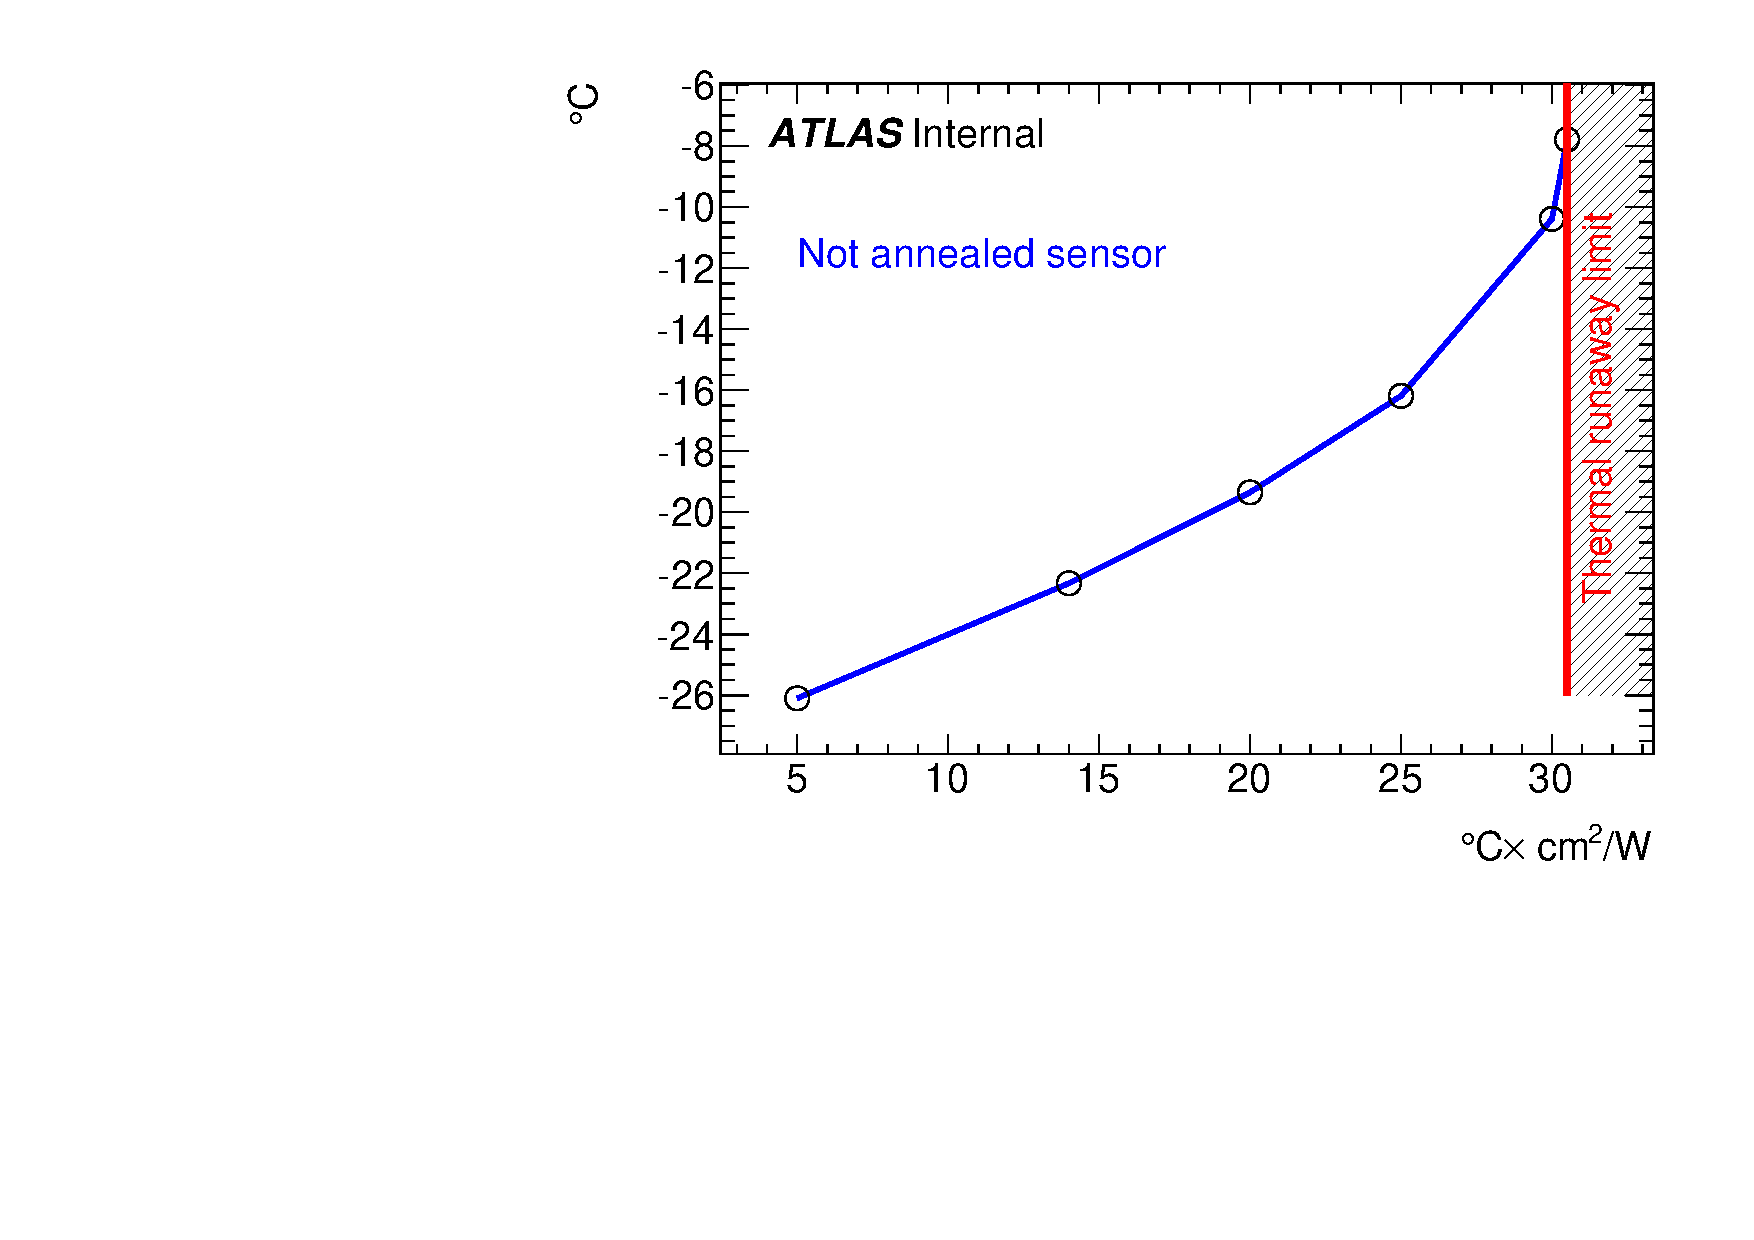
\includegraphics[width=0.6\textwidth]{Images/IBL_Paper/chapter05_Staves/ThermalRunAway.pdf}
\caption{Sensor maximum temperature  with respect to the stave thermal figure of merit $TFoM$ at \SI{-40}{\celsius} evaporative cooling temperature.}
\label{fig:ThermalRunAway}
\end{center}
\end{figure}

A validation of the simulation is  illustrated in the  graph reported in Figure~\ref{fig:Temperature}a that shows the thermal results obtained on a stave prototype during the final design qualification. The $TFoM$ measured is  \SI{14}{\celsius \centi\meter^2\per\watt} for $T_{coolant} = \SI{-22}{\celsius}$ which is conservatively two times below the admissible value. To qualify the  stave thermal performance during the  production, temperature uniformity has been measured after module loading. All installed staves shows a temperature dispersion within \SI{0.48}{\celsius}, as shown in Figure~\ref{fig:ModuleTemperature}, which is a good indication of the production uniformity. \\

\begin{figure}
        \centering
        \subfloat[\label{fig:TemperatureProfile}]{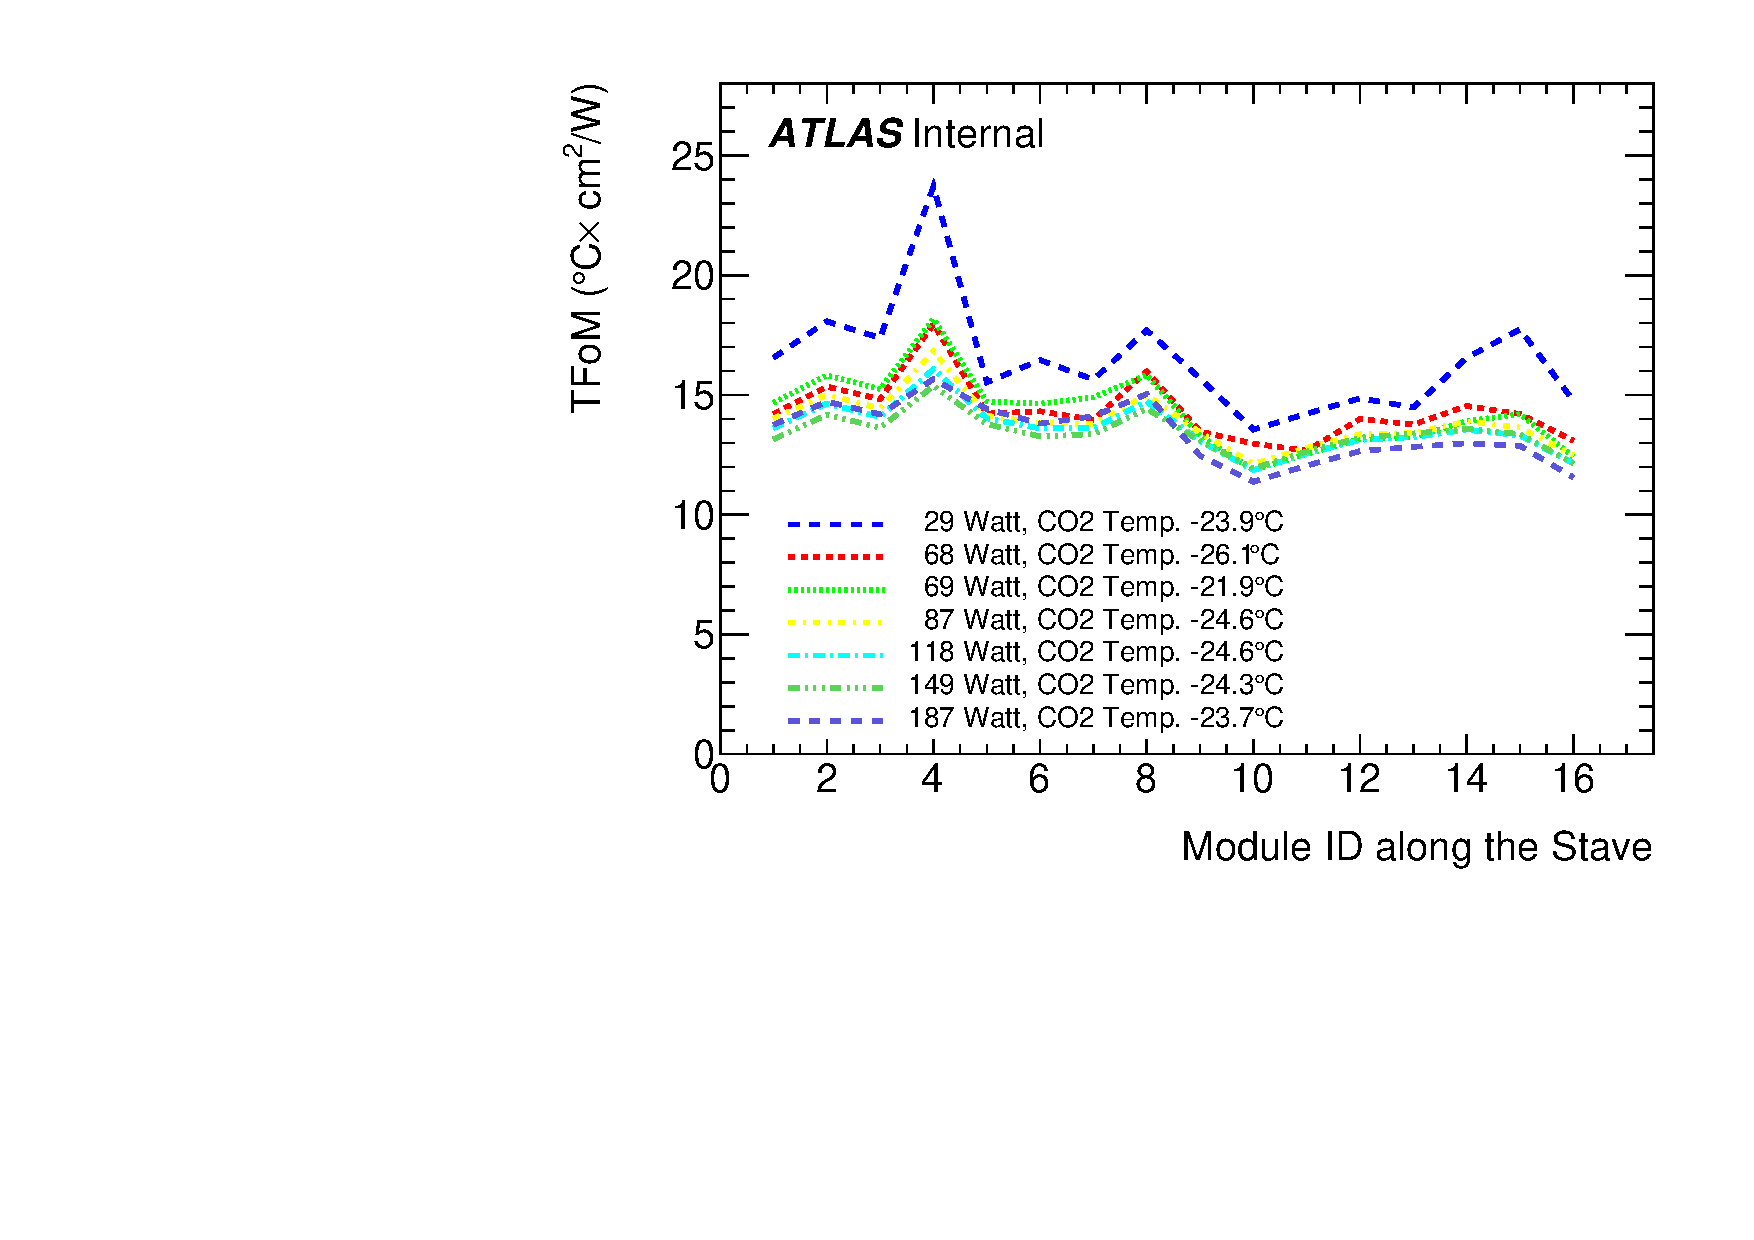
\includegraphics[width=0.47\textwidth]{Images/IBL_Paper/chapter05_Staves/TemperatureProfile.pdf}}
        \subfloat[ \label{fig:ModuleTemperature}]{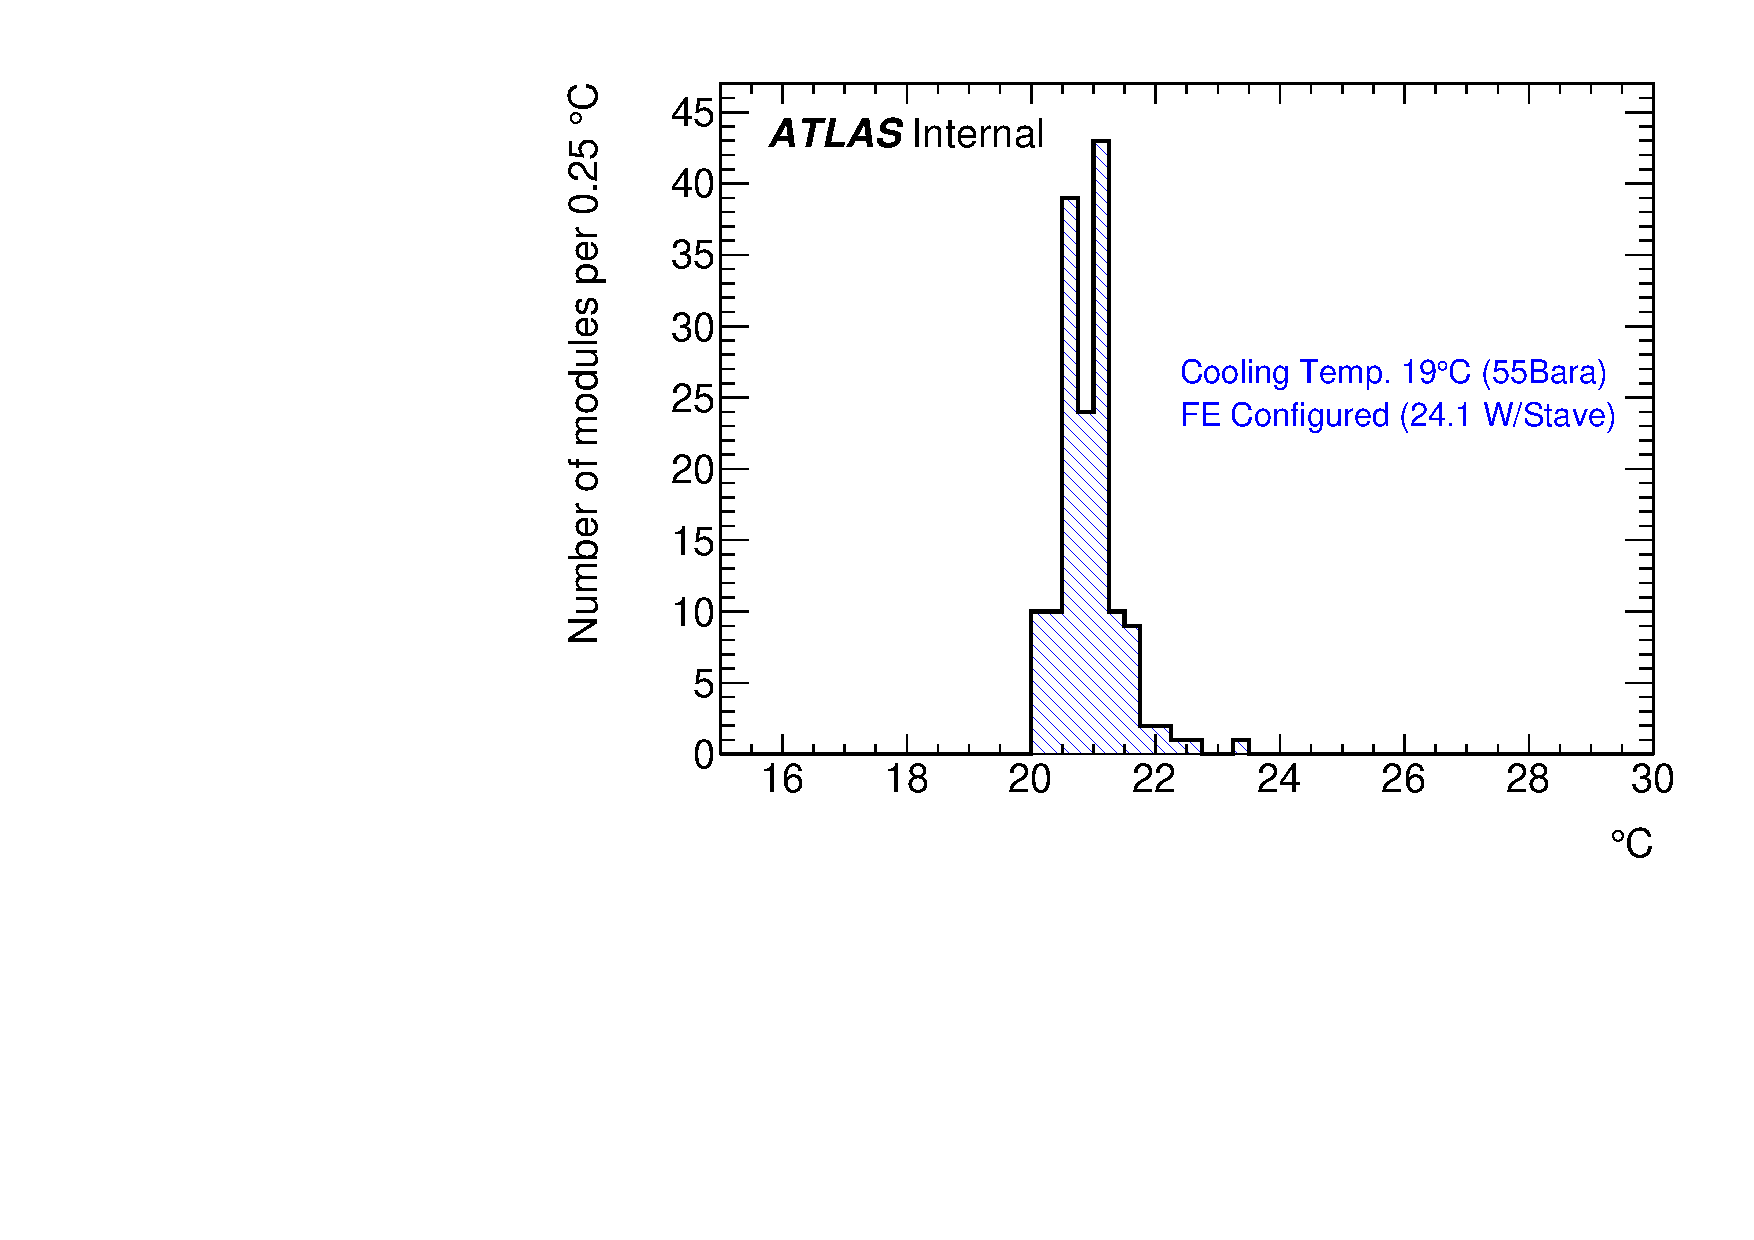
\includegraphics[width=0.47\textwidth]{Images/IBL_Paper/chapter05_Staves/ModuleTemperature.pdf}}
  \caption{a) $TFoM$ of \SI{1.5}{\milli\meter} cooling tube stave along the cooling line. b) Module temperature distribution on produced staves with a cooling temperature of \SI{19}{\celsius} and read-out electronics configured. The histogram has 152 entries, a mean value of %\SI{20.9}{\degrees\celsius} and a RMS of \SI{0.5}{\degrees\celsius}.}
  \SI{20.9}{\celsius} and a RMS of \SI{0.5}{\celsius}.}
  \label{fig:Temperature}
\end{figure}

%\subsubsection{Quality control and production}
%The bare stave production is a 13-steps process which requires careful quality control to standardise the production.  The bare stave quality control was performed as follow:
%\begin{itemize}
%\item   Visual inspection to check for cracks or strips or mechanical unconformities
%\item   Full metrological control (especially assembly pin hole dimensions and distance and stave global Planarity)
%\item   Weight control
%\item   \SI{150}{\bar}(a) pressure test and He leak check.
%\end{itemize}
%In total 33 staves were produced, and a similar number of prototypes were built to verify the design performance and to tune the production process. Table~\ref{tab:staveFailureRate} summarises the yield of the bare stave production.


%\begin{table}[!htb]
%\centering
%\begin{tabular}{l c  }
%\hline \hline
%        Type & \#      \\
%\hline
%Bare staves produced & 33 \\
%Staves rejected after Visual Inspection & 7 \\
%Staves used as prototypes & 2 \\
%Staves rejected after high pressure and He leak test & 0 \\
%Staves rejected after metrology & 0 \\
%Staves accepted for flex assembly  & 24 \\
%\hline
%Total Failure Rate:             & \SI{27}{\percent} \\
%\hline \hline
%\end{tabular}   
%\caption{Bare stave failure rate during QA.
%\label{tab:staveFailureRate}}
%\end{table}
%
%The staves weight was systematically checked to control the manufacturing uniformity. The weight is a good indication of the amount of glue used which has a non-negligible impact on the radiation length. On the production staves, the average total stave weight is \SI{26\pm1}{\gram}.
%The bare stave Planarity is an important factor which has been carefully controlled. This parameter, which belongs to the selection criteria (admissible value set to \SI{0.250}{\milli\meter} along the stave length) impacts the module loading activity and the minimum gap between two adjacent stave around the beam-pipe. Figure~\ref{fig:BareStavesPlanarity} reports the mean Planarity  on all the produced staves, by measurements along the staves profile and in three radial positioning, thus showing an evident snake profile.
%
%\begin{figure}[!htb]
%\begin{center}
%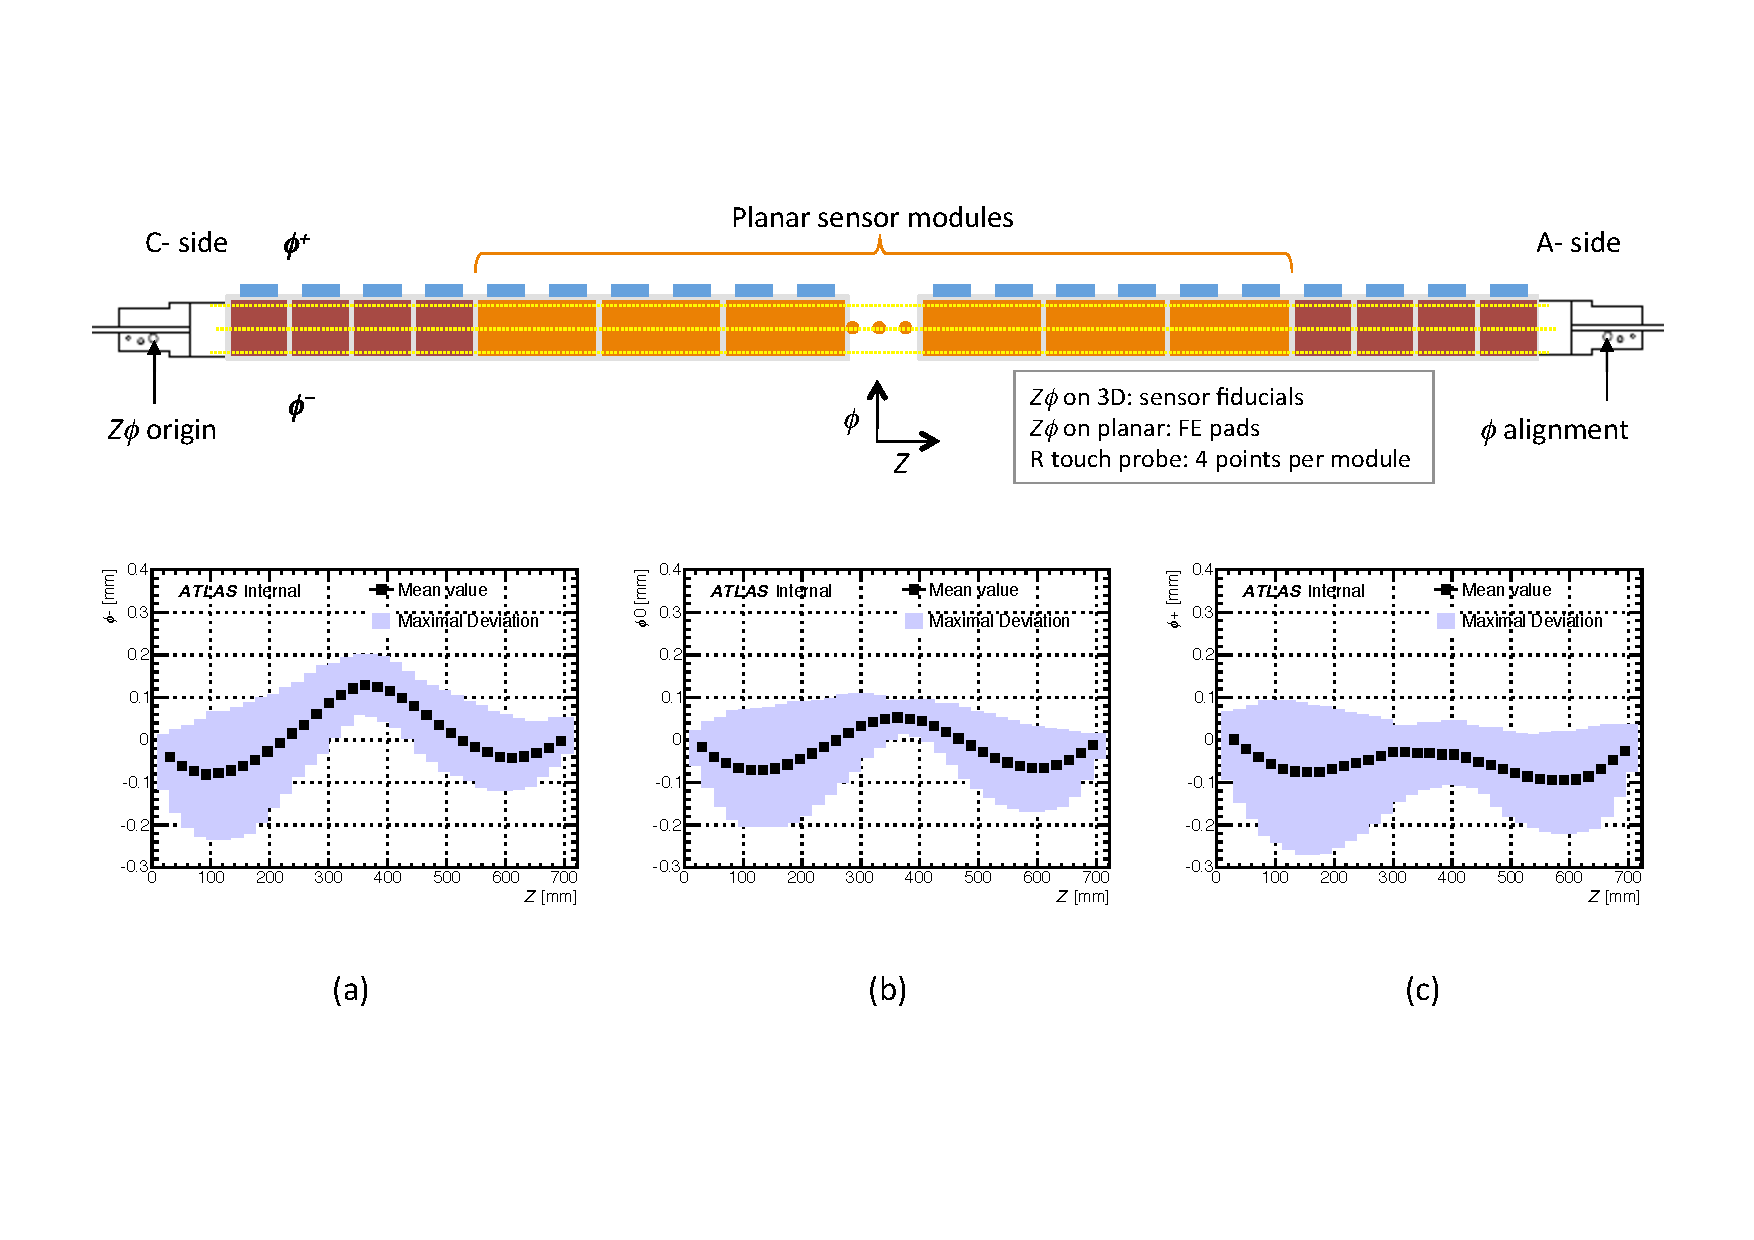
\includegraphics[width=0.9\textwidth]{Images/IBL_Paper/chapter05_Staves/StaveMetrologyLayout3.pdf}
%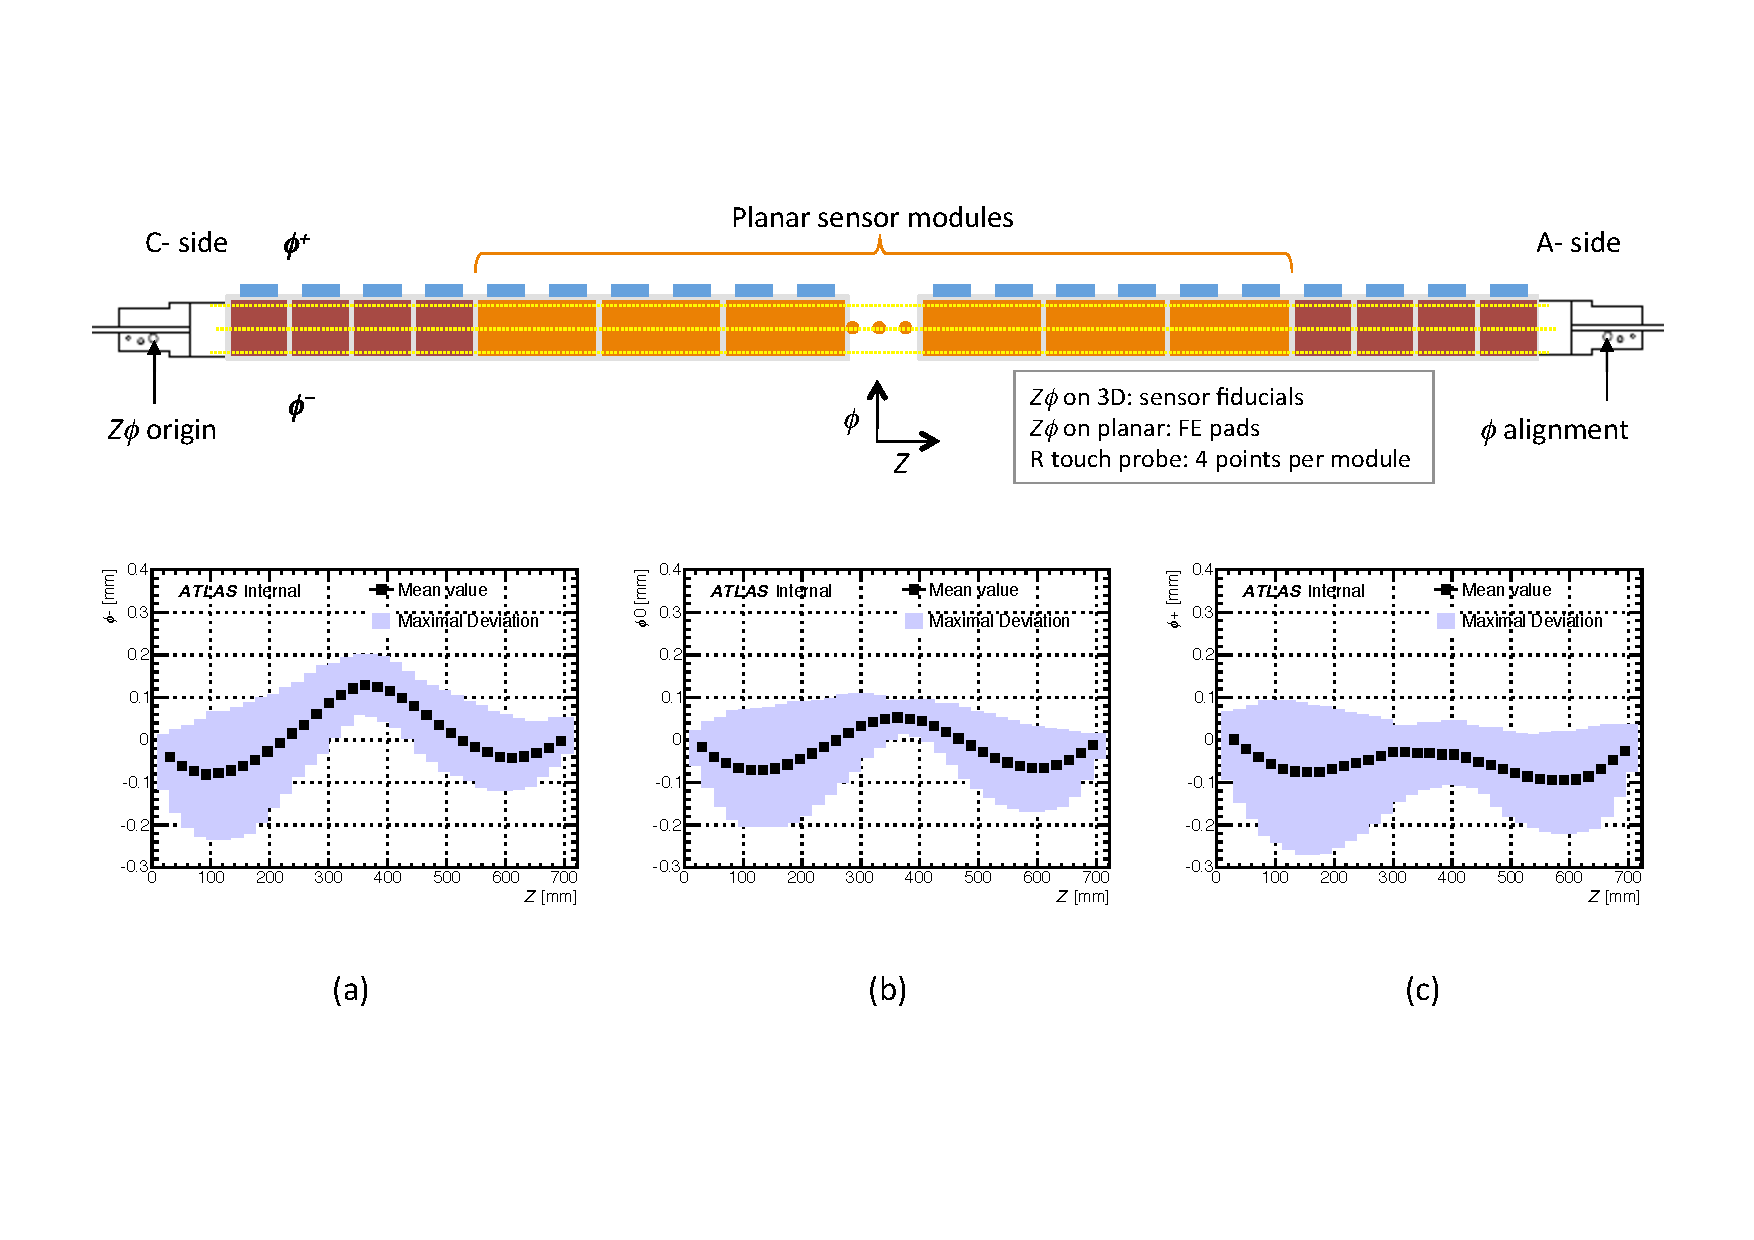
\includegraphics[width=0.8\textwidth]{Images/IBL_Paper/chapter05_Staves/BareStavesPlanarity.pdf}
%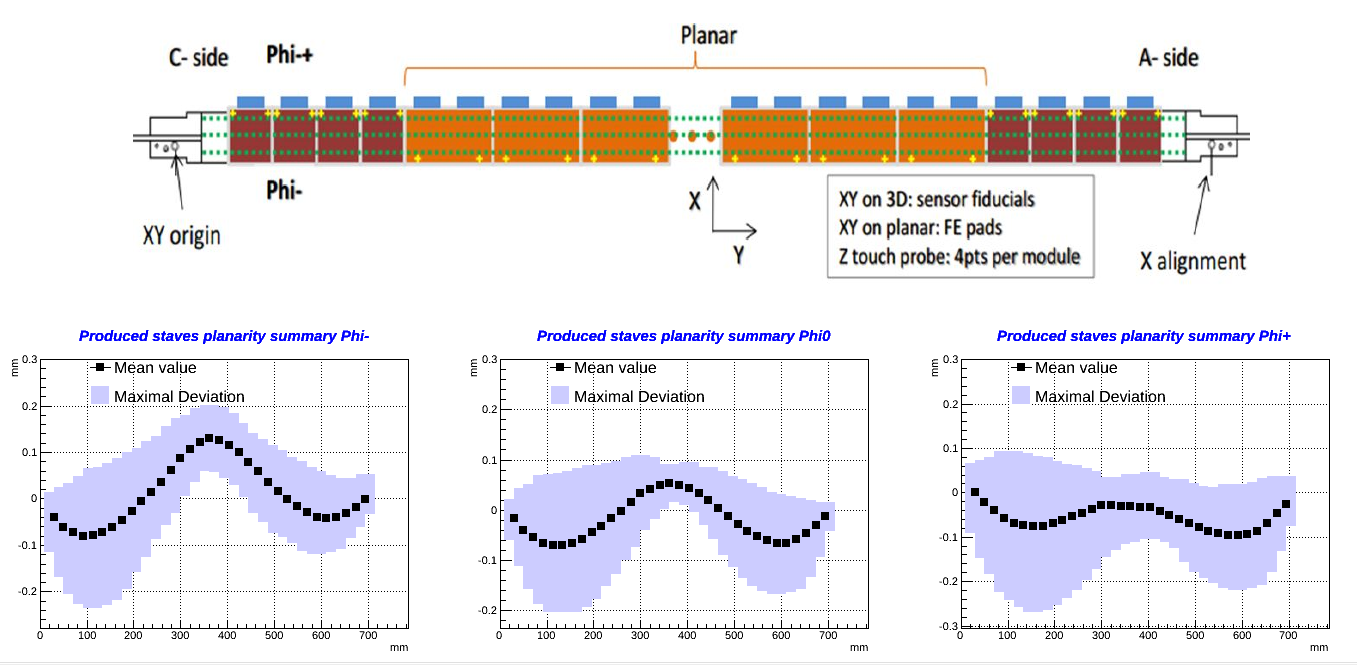
\includegraphics[width=0.9\textwidth]{Images/IBL_Paper/chapter05_Staves/jffagidg.png}
%\caption{Bare staves Planarity summary for the production bare staves in three azimuthal positions, at the stave edges  and central position: the error bars show the RMS spread, while the solid boxes show the minimum and maximum values.}
%\label{fig:BareStavesPlanarity}
%\end{center}
%\end{figure}
%
%
%\subsection{Stave flex: Quality control and production}
%The flex production was organized in batches of 2-4 sheets with three flexes each, all of the same type, either C or A.  After the produced  flexes were singled out, they were cleaned after having loaded the connectors and then shipped to the qualification laboratory. The qualification consists of:
%
%\begin{itemize}
%\item Visual inspection: to spot mechanical damages and surface anomalies,
%\item First electrical test: resistance measurements, continuity check and short search,
%\item Wings bending: araldite gluing at room temperature of the 16 wings, mechanical measurements,
%\item   Quick electrical test: continuity check,
%\item   Ten thermal cycles (\SI{-40}{\celsius} to \SI{40}{\celsius}),
%\item   HV test: at least one day at \SI{1500}{\volt} with current limit at \SI{0.1}{\micro\ampere},
%\item   Final electrical test: resistance measurements, continuity check and short search,
%\item   Final visual inspection and sign-off for delivery.
%\end{itemize}
%%
%Table~\ref{tab:flexstaveFailureRate} reports the stave flex yield.  
%Several flexes were rejected during production by the vendor, mainly at the very beginning of the production,  because of electrical or mechanical non-conformity. Of the 61 accepted flexes, a qualitative ranking has been made  according to their electrical performance or mechanical conformity. The main reason for lower ranking has been high resistivity in the vias. Several sources of lower ranking have been identified, mainly small non-conformities during the visual inspection. Figure~\ref{fig:FlexResults1} shows the evolution with time of the resistance of the LV lines between the connectors and the wing pads, while Figure~\ref{fig:FlexResults2} shows the LV resistance between two adjacent wings, that is dominated by the vias resistance. The decrease of the resistance is due to a better control in the flex production and metallisation processes. For the round trip  LV voltage drop assuming a 2A current,  \SI{\sim320}{\milli\volt} in the last batches, the critical parameter is the resistivity of the LV lines. However a high inter-wing resistivity, without affecting the LV requirements, could point to a weak connection. For this reason, affected flexes have been rejected. \\
%Finally, electrical tests have been repeated at CERN before and after gluing on the stave. Only on one stave, a  small HV resistivity change has been observed, but the stave flex has not been rejected. 
%
%
%
%\begin{figure}[!hthb]
%\begin{center}
%	\begin{subfigure}[t]{0.47\textwidth}
%		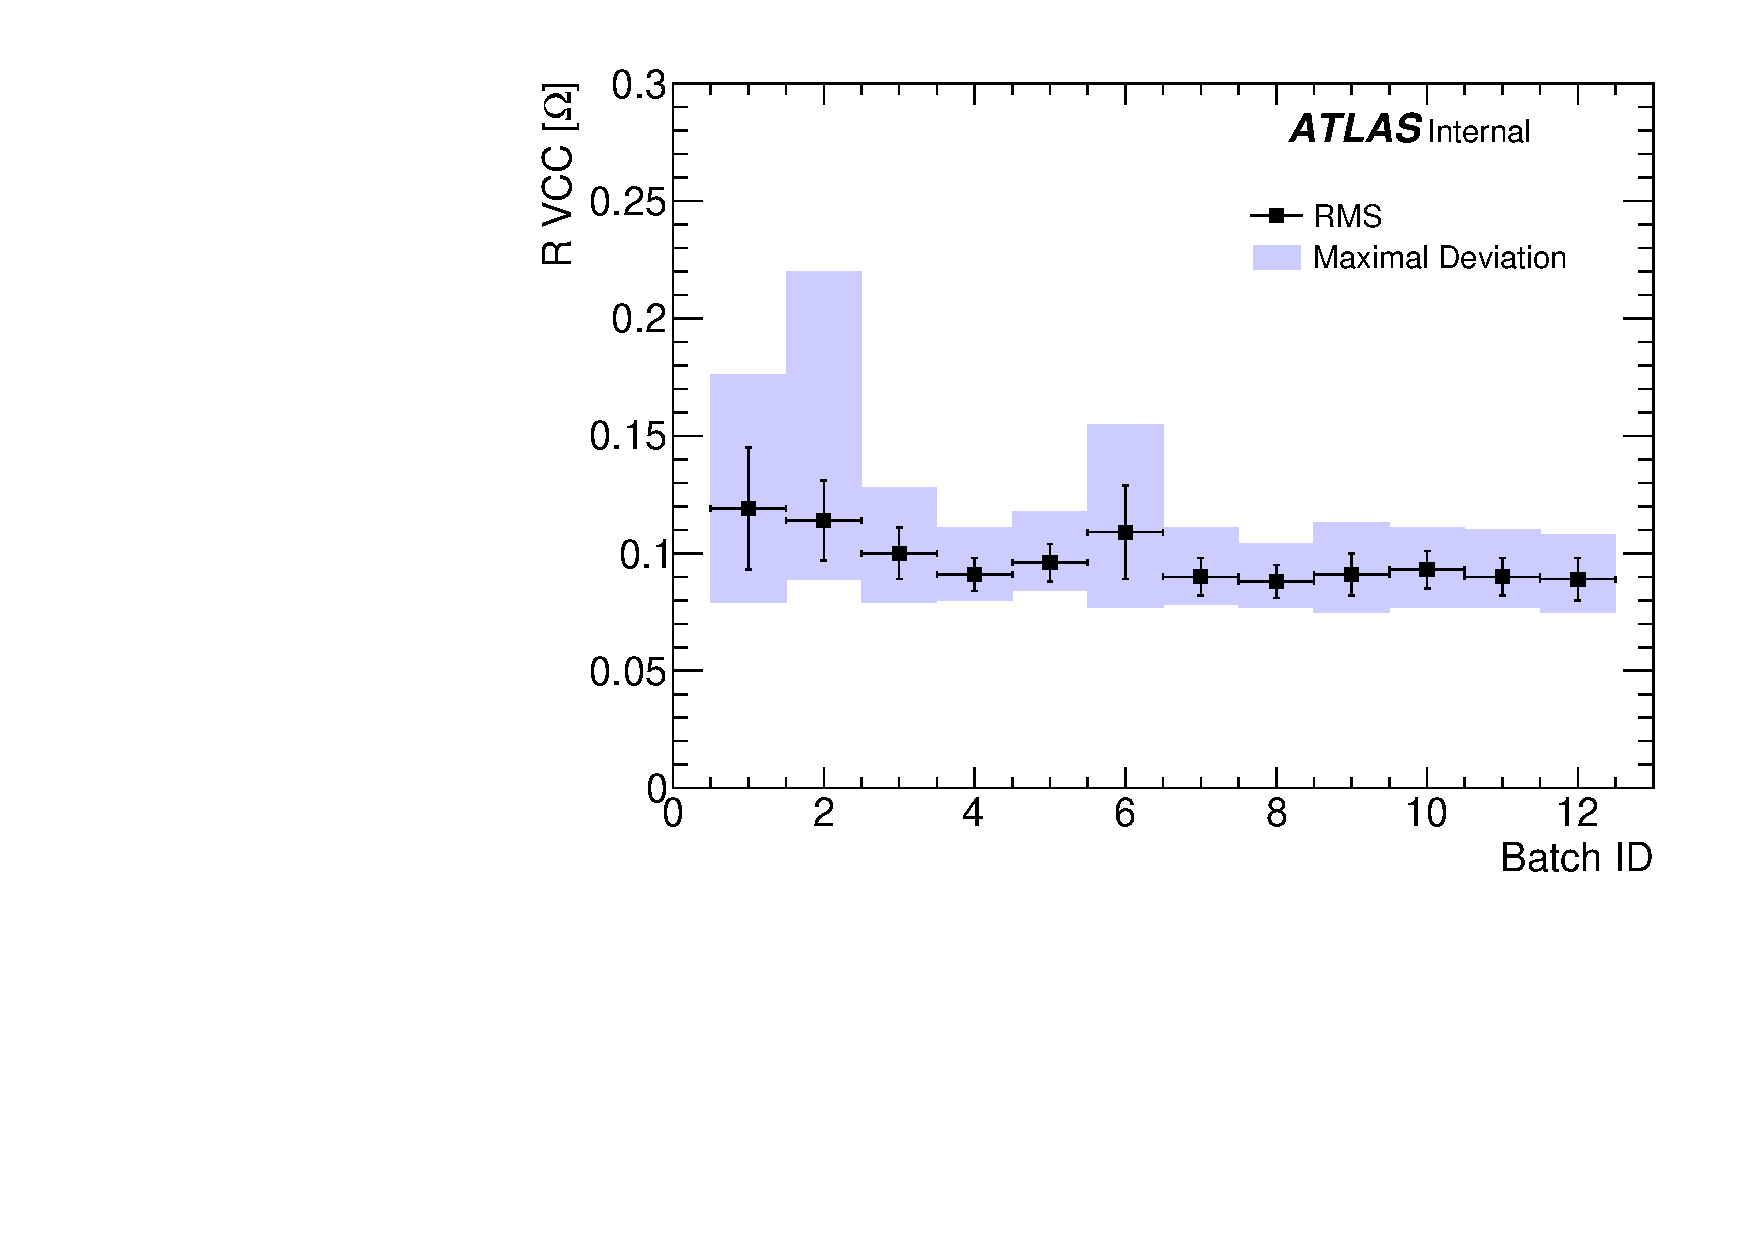
\includegraphics[width=0.47\textwidth]{Images/IBL_Paper/chapter05_Staves/VCC.pdf}
%		\caption{}
%		\label{fig:FlexResults1a}
%	\end{subfigure}
%	\begin{subfigure}[t]{0.47\textwidth}
%		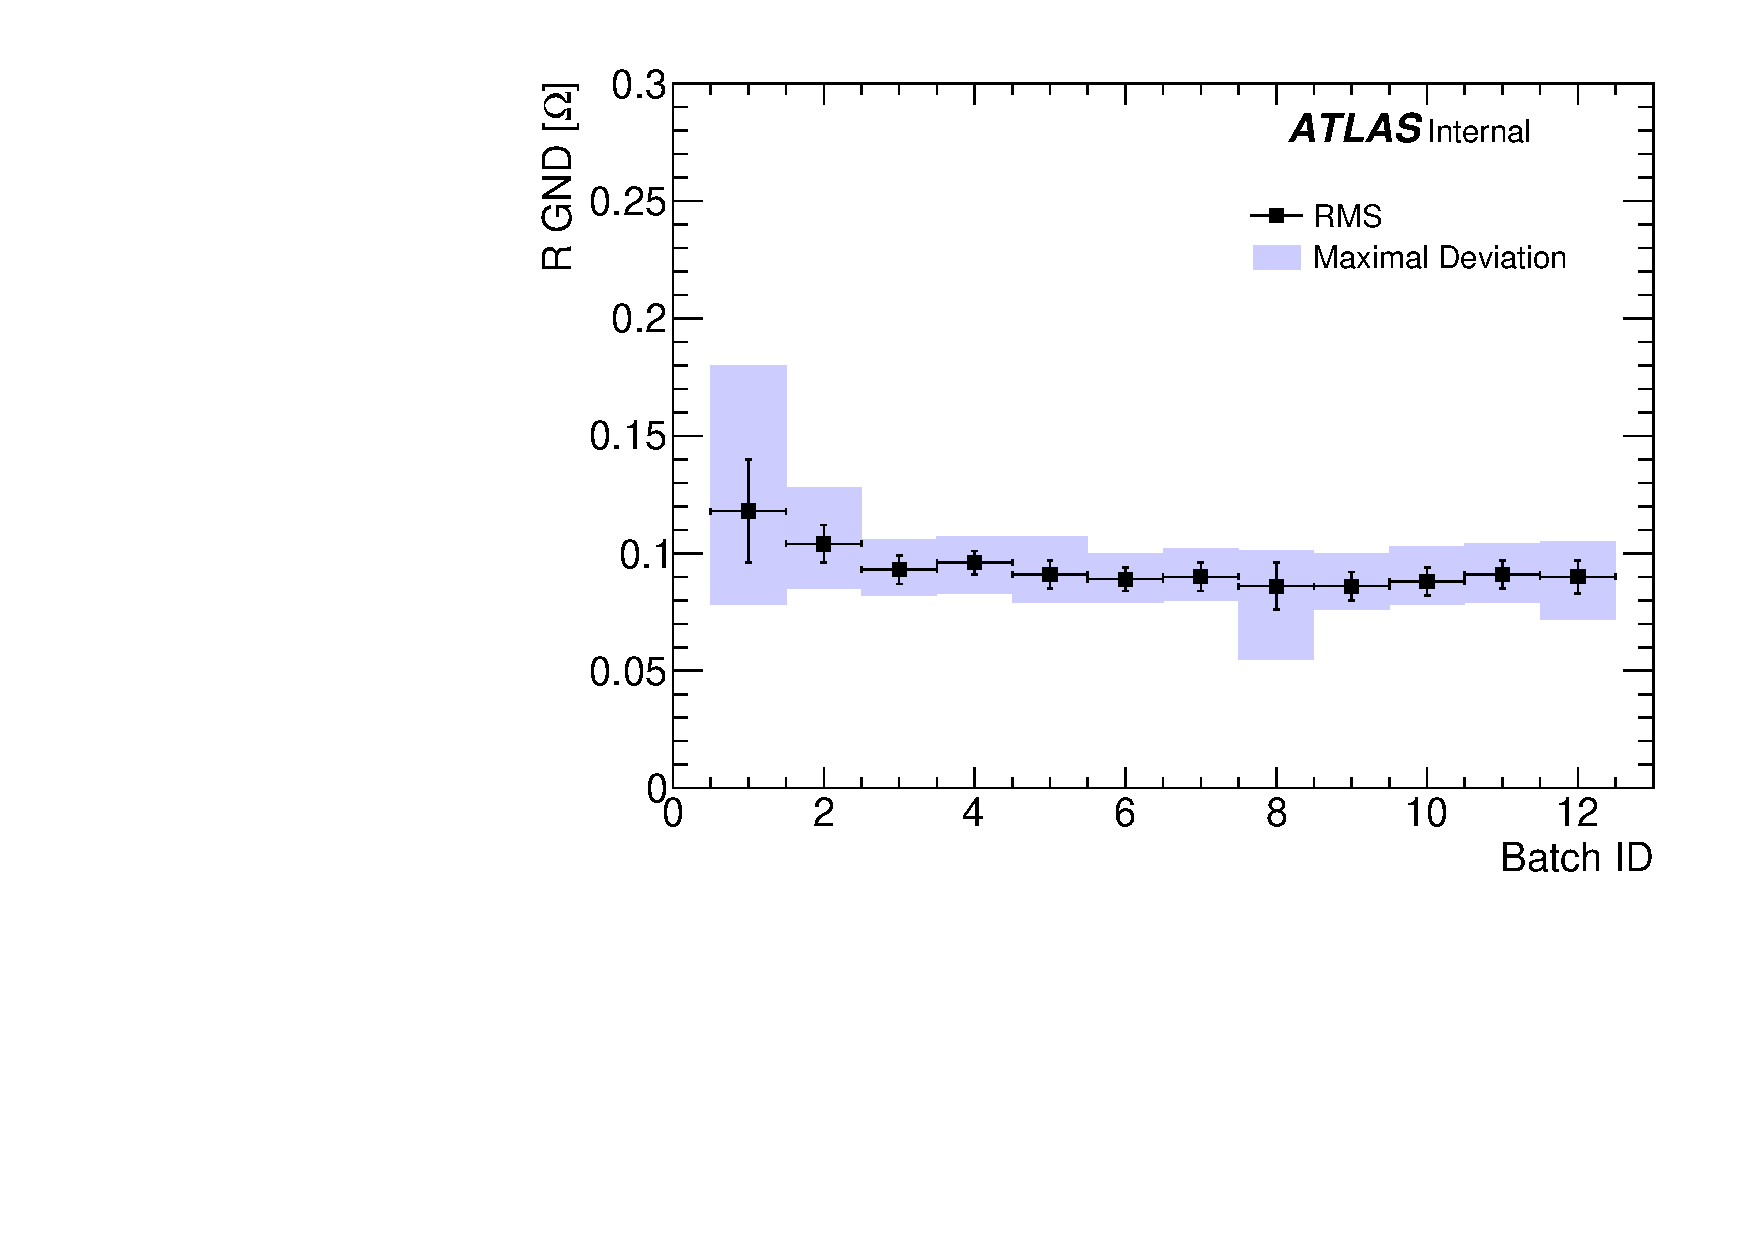
\includegraphics[width=0.47\textwidth]{Images/IBL_Paper/chapter05_Staves/GND.pdf}
%		\caption{}
%		\label{fig:FlexResults1b}
%	\end{subfigure}
%\caption{
%Resistance as a function of batch delivery date for (a) the VCC and (b) the GND lines measured between the EOS and each wing. The quoted resistance is the average of 16 measurements per flex on successive production batches, each of 6  flexes. 
%\label{fig:FlexResults1}}
%\end{center}
%\end{figure}
%
%\begin{figure}[!hthb]
%\begin{center}
%	\begin{subfigure}[t]{0.47\textwidth}
%		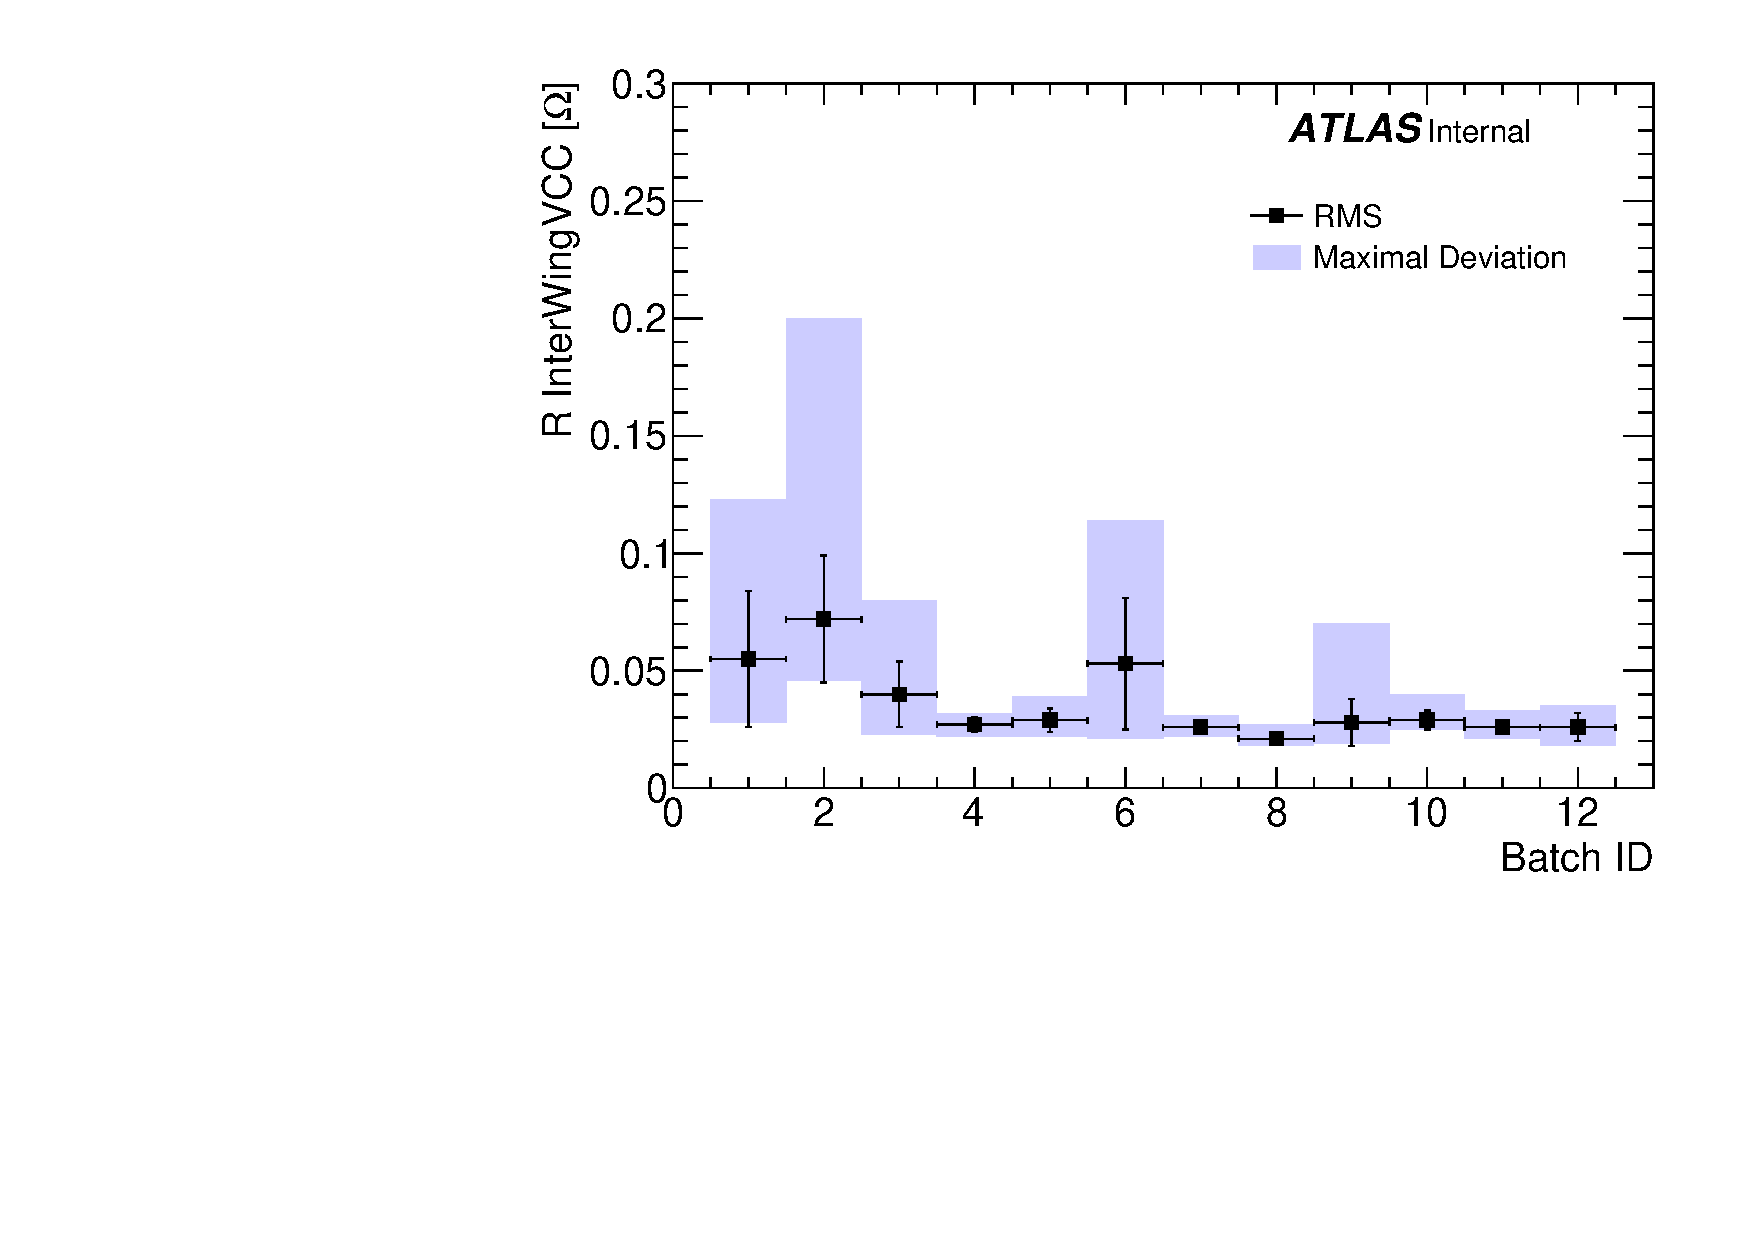
\includegraphics[width=0.47\textwidth]{Images/IBL_Paper/chapter05_Staves/InterWingVCC.pdf}
%		\caption{}
%		\label{fig:FlexResults2a}
%	\end{subfigure}
%	\begin{subfigure}[t]{0.47\textwidth}
%		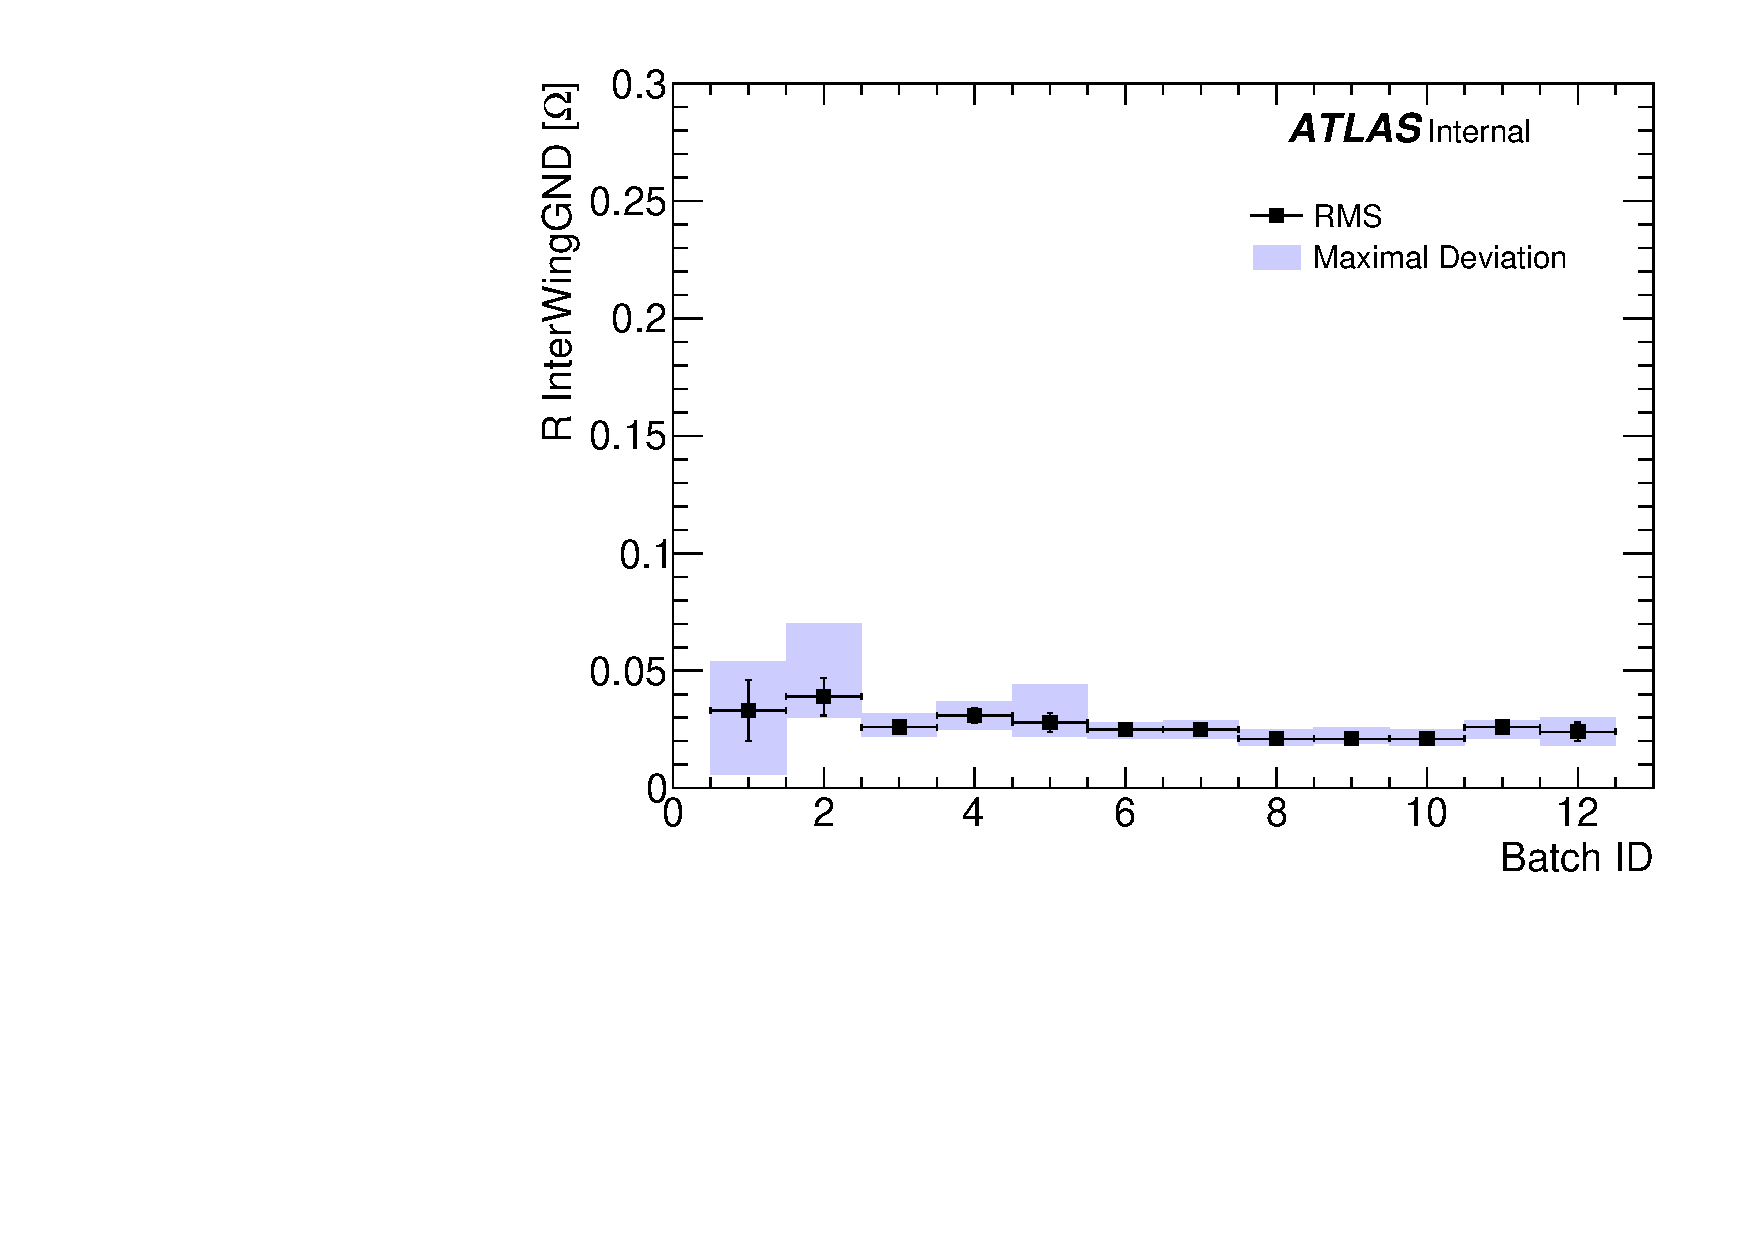
\includegraphics[width=0.47\textwidth]{Images/IBL_Paper/chapter05_Staves/InterWingGND.pdf}
%		\caption{}
%		\label{fig:FlexResults2b}
%	\end{subfigure}
%%\begin{tabular}{cc}
%%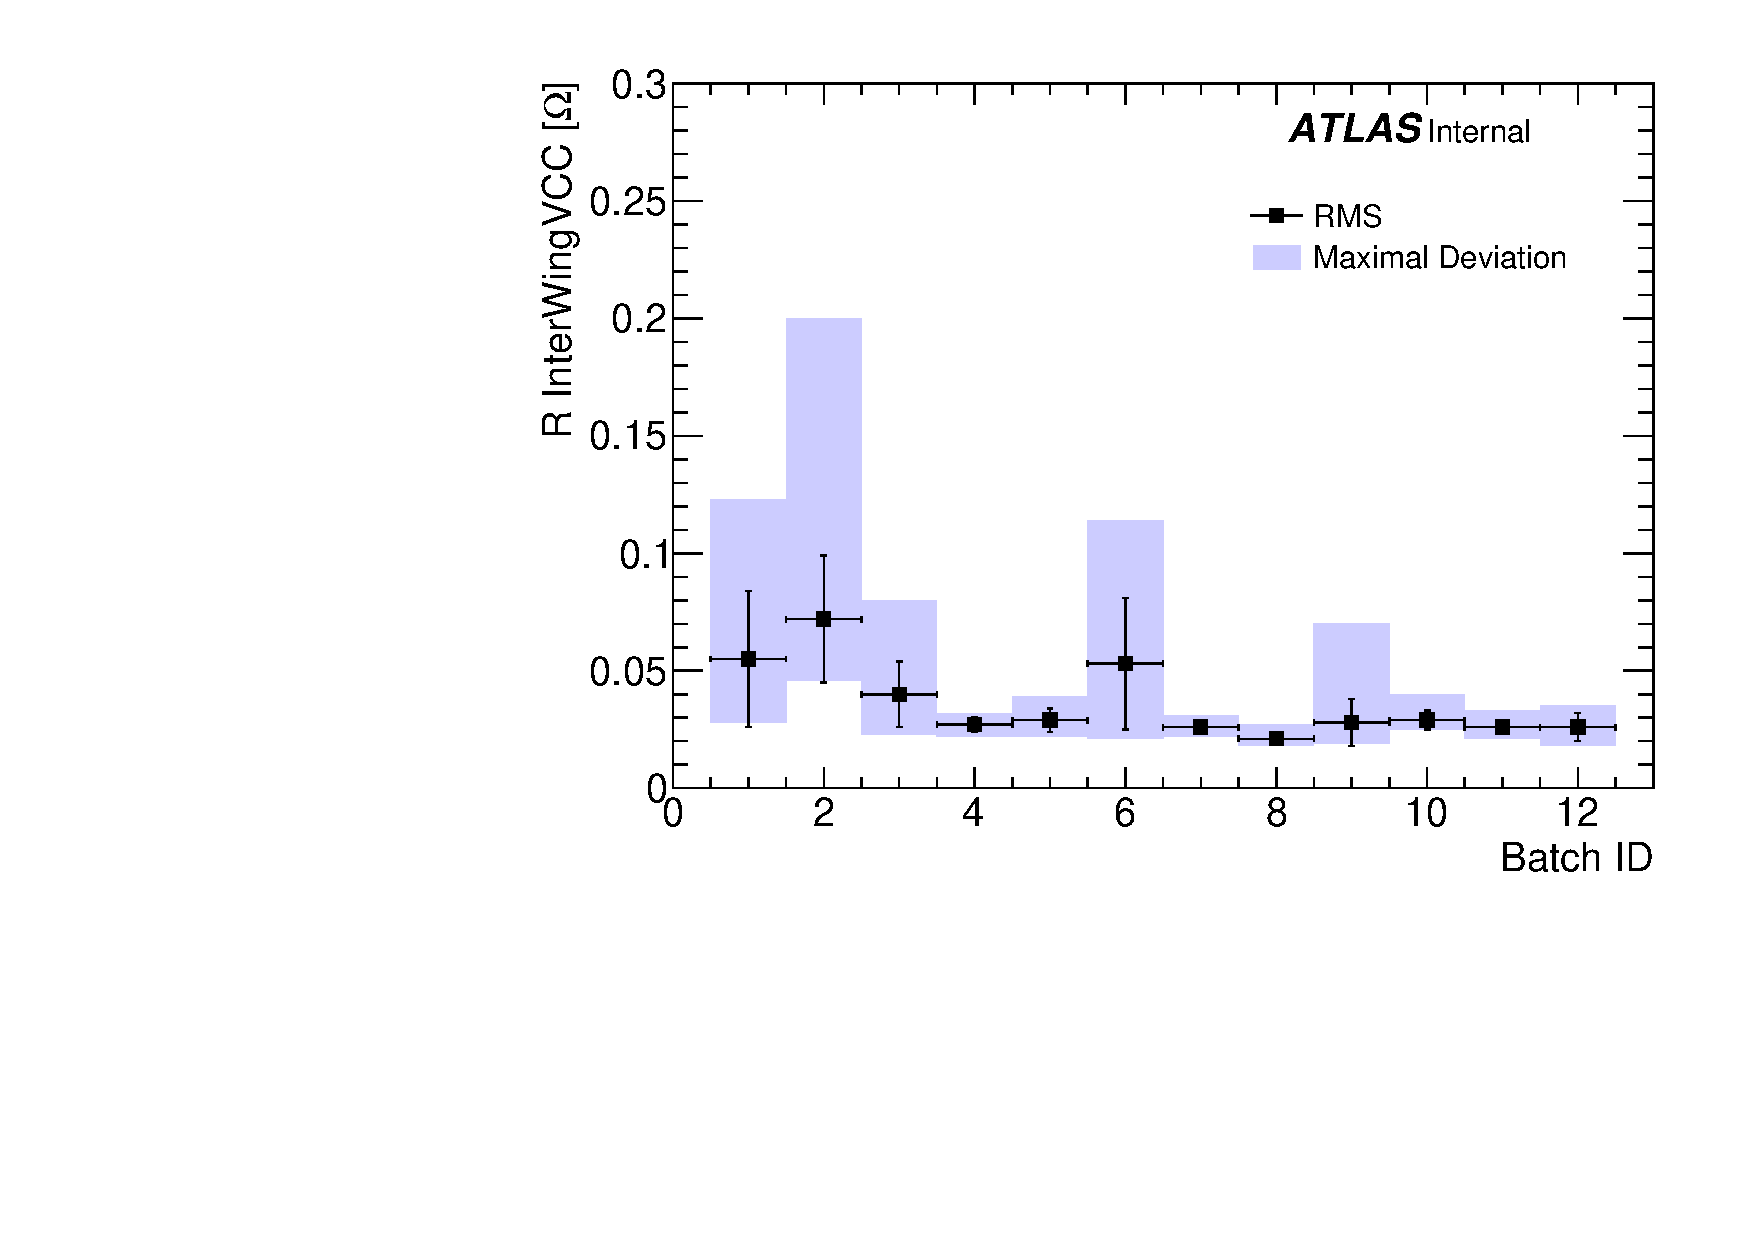
\includegraphics[width=0.5\linewidth]{Images/IBL_Paper/chapter05_Staves/InterWingVCC.pdf} &
%%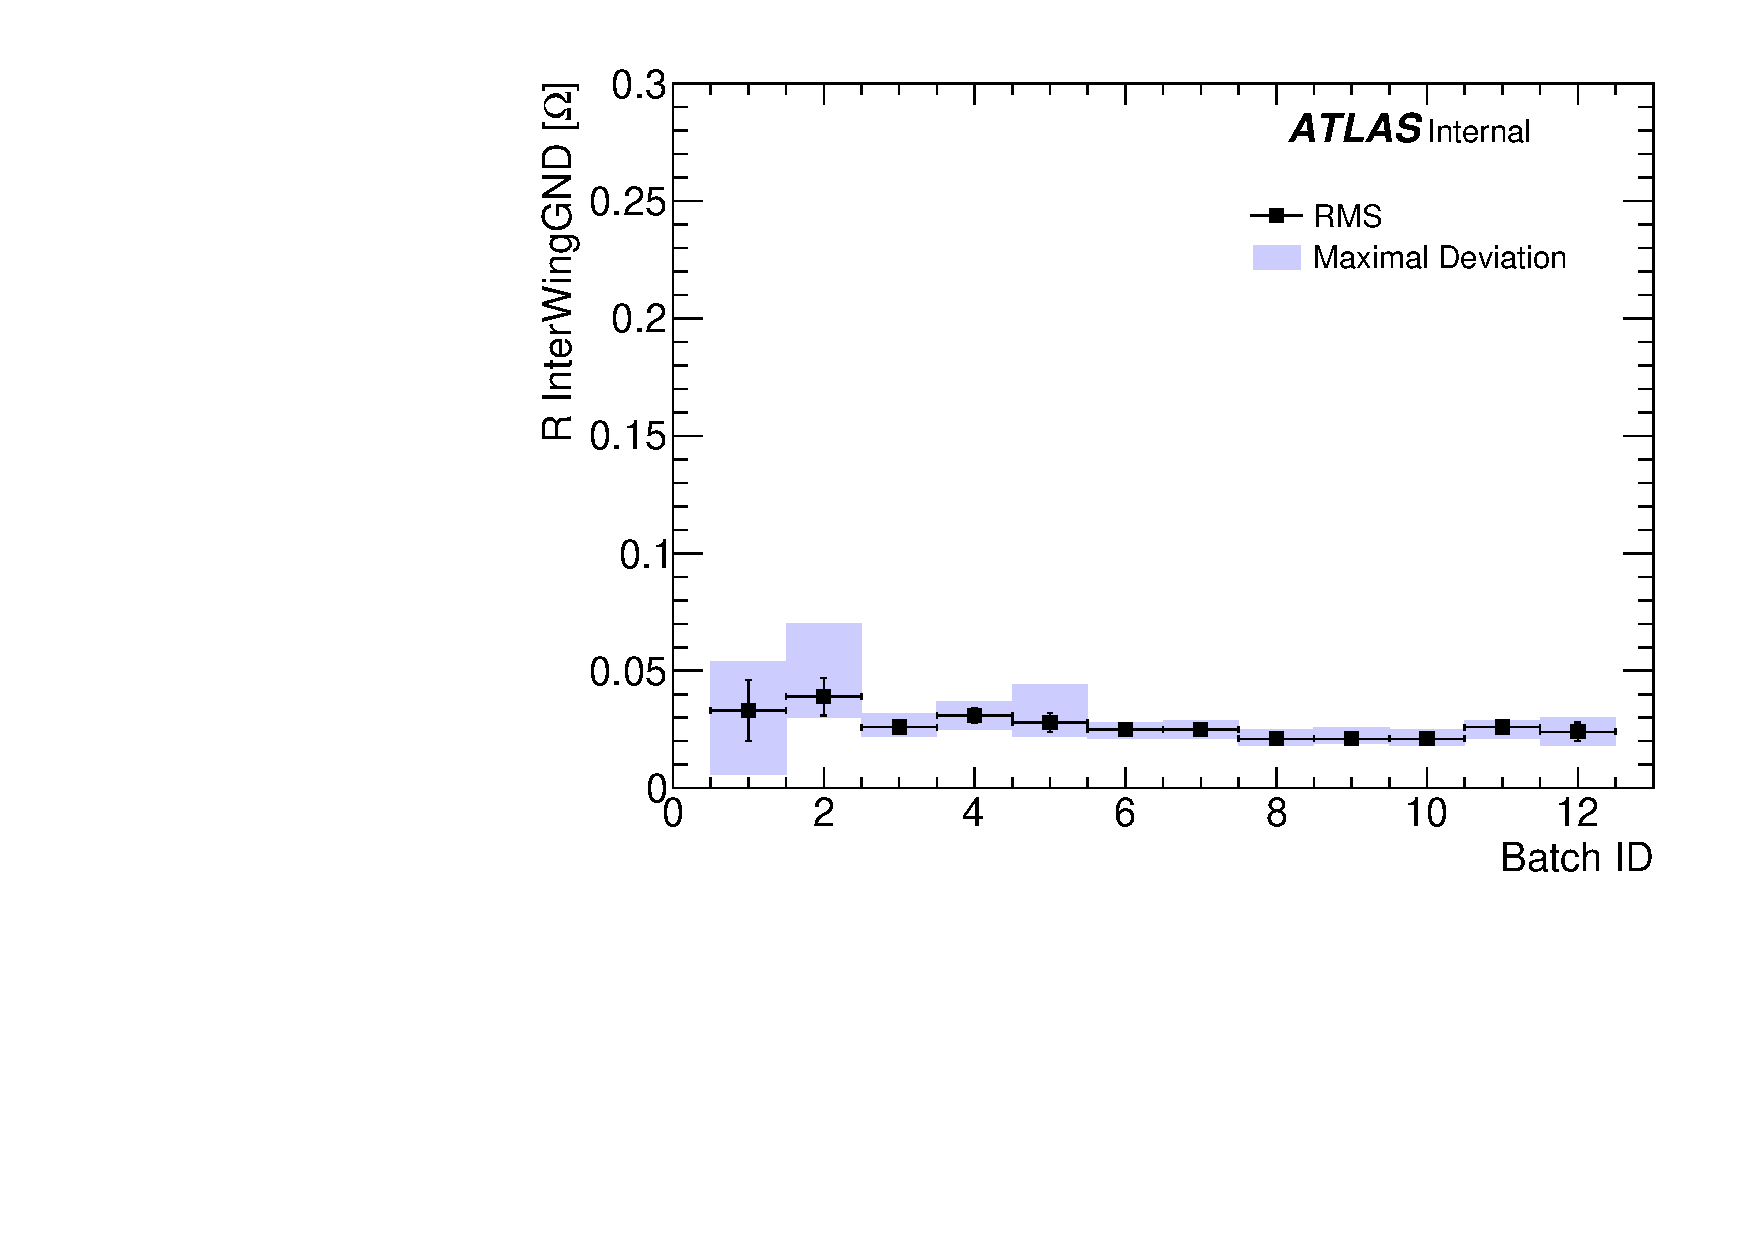
\includegraphics[width=0.5\linewidth]{Images/IBL_Paper/chapter05_Staves/InterWingGND.pdf} \\
%%\end{tabular}
%\caption{
%Resistance as a function of batch delivery date for (a) the VCC and (b) the GND lines measured  between two adjacent wings - so called inter-wing. The quoted resistance is the average of 12 measurements per flex on successive production batches, each of 6  flexes. 
%\label{fig:FlexResults2}}
%\end{center}
%\end{figure}
%
%
%\begin{table}[!htb]
%\centering
%\begin{tabular}{l c  }
%\hline \hline
%        Type & \#      \\
%\hline
%Stave flexes produced & 72 \\
%Flexes rejected during production  & 6 \\
%Flexes rejected after visual inspection & 2 \\
%Flexes rejected after the electrical test & 2 \\
%Flexes rejected after the HV test & 1 \\
%Flexes rejected after the thermal cycles & 0 \\
%Flexes rejected due to mishandling  & 0 \\
%Stave flexes accepted for loading  & 61 \\
%\hline
%Total Failure Rate:             & 15\% \\
%\hline \hline
%\end{tabular}   
%\caption{Stave flexes failure rate during QA.
%\label{tab:flexstaveFailureRate}}
%\end{table}
%

\subsubsection{Stave Flex}
\begin{figure}
{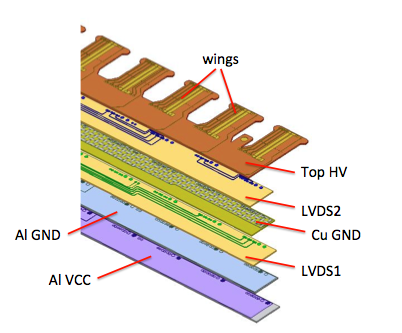
\includegraphics[width=0.6\textwidth]{Images/IBL_paper/chapter05_Staves/FlexStack3D.png}}
%\subfloat[fig:FlexScheme]{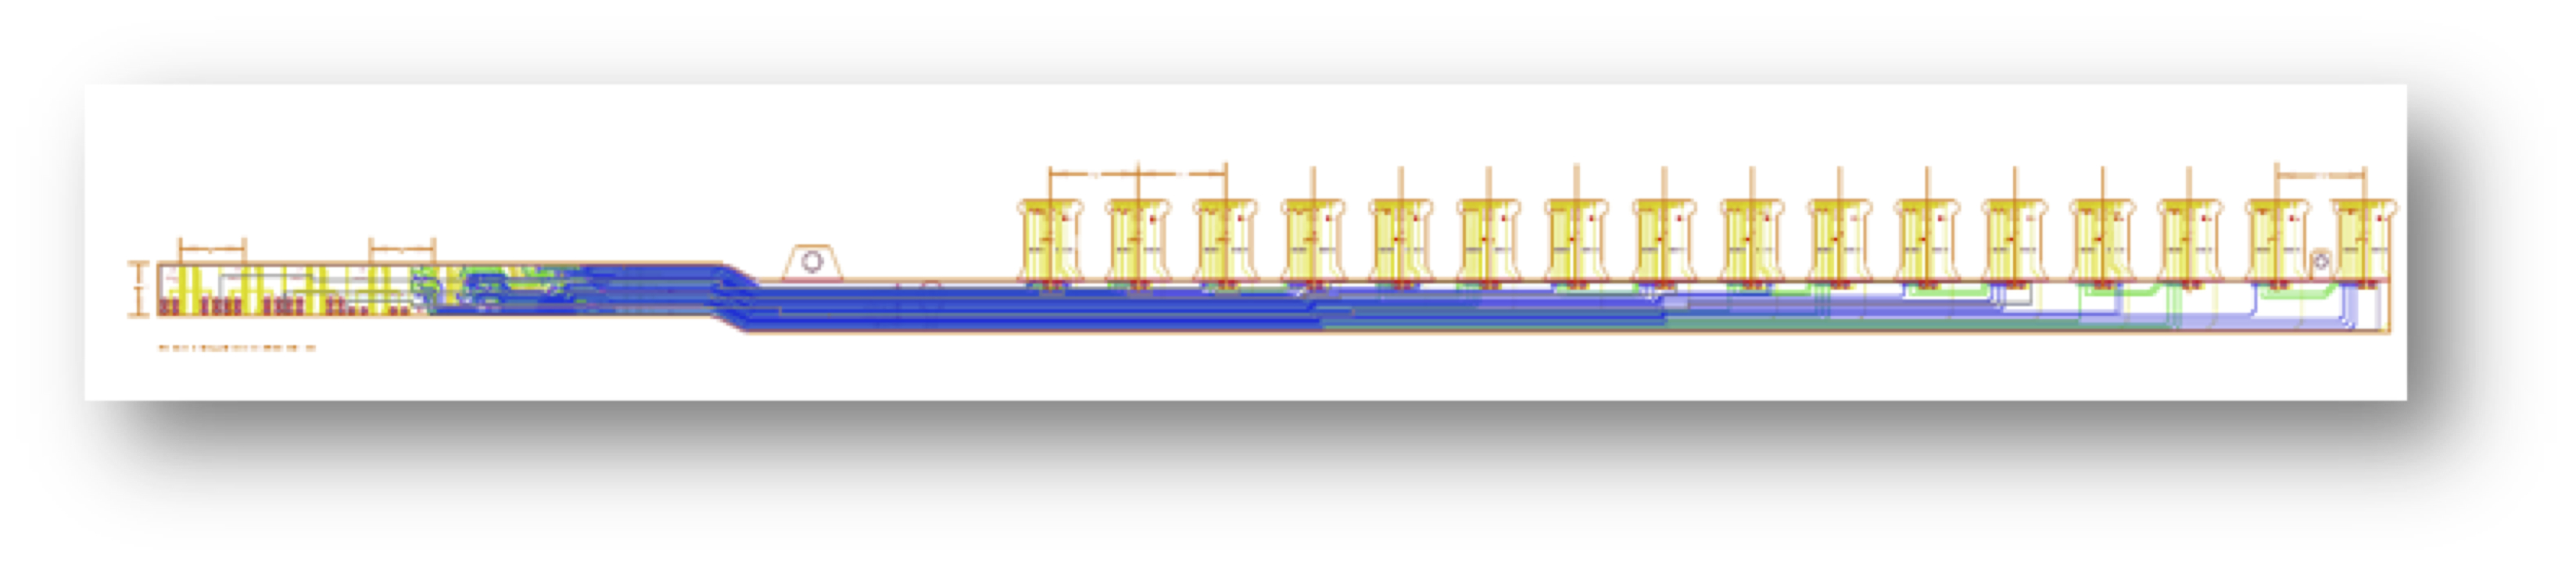
\includegraphics[width=0.6\textwidth]{Images/IBL_paper/chapter05_Staves/FlexLayout.jpg}}
\caption{Stack of the different layer of the stave flex. }
\label{fig:Flex3D}
\end{figure}
Two symmetric multi-layer flexible circuits, the stave flexes, are glued on the back of the mechanical support structure and route electrical services to the end of stave regions. A stack of the different layers of the stave flex is shown in Figure~\ref{fig:Flex3D}
Each stave flex has 16 lateral extensions, one per front-end chip, so-called wings, that mechanically and electrically connect the module and the stave flex. 
The glueing required a positional accuracy of \SI{0.3}{\milli\meter} in the longitudinal direction and of \SI{0.1}{\milli\meter} in the transverse direction of the stave in order to fit with the IBL envelope requirement.
The harsh radiation environment, the thermo-mechanical constrains and the minimization of the material budget are fundamental condition for the choice of the glue to be used. After an intensive campaign of test the Araldite 2011 was selected as best option.
Both thermal and radiation loads were applied to the stave assembly during a test campaign with a 10MeV electron source. After an irradiation of \SI{380}{\mega\radian} and 110 thermal cycles between \SI{40}{\celsius} and \SI{-40}{\celsius} no critical damage was observed on the stave-flex glue joint\cite{BilbaodeMendizabal:1557832}.

\clearpage


